\chapter{Method}\label{ch:method}

\begin{itemize}
    \item Method is probably not the right title here, it's more "Foundations" or something like that.
        Maybe give some introduction to this chapter that your goal is to present the basics necessary for XPBD and 
        PD and maybe a teaser how optimization is need etc., a bit of an outline of the chapter.
    \item While citing books, put chapters into the citations.
\end{itemize}

\section{Time-Integration of Physical Systems}\label{s:physical-integration}
\textcolor{red}{Fabian recommends citing \cite{gast2015}.}

In most approaches for the simulation of physical systems, the motion of the system is assumed to be in accordance with Newton's laws of
motion. \textcolor{red}{Maybe list all of them. Newton's first law is definitely going to be mentioned, not sure about the third one. I
don't want to spend too much time on contact.} Due to Newton's second law 

\begin{equation}\label{newtons-laws-2}
    \vecm{f} = m\vecm{a},
\end{equation}

\noindent it is possible to relate the force $\vecm{f}$ acting on a particle and the resulting acceleration $\vecm{a}$ via the particle
mass $m$. The motion of a particle system can then be described in terms of a system of ordinary differential equations (ODEs). This
system of ODEs is commonly referred to as the equations of motion. The equations of motion are integrated over time in order to arrive 
at the configuration of the system at the next time step. For general forces, finding an analytical solution to the equations of motion
is impossible and numerical integration schemes must be employed instead. In particular, both XPBD (\cref{ss:xpbd-constraint-projection}) 
and PD (\cref{ss:pd-solver}) are based on a numerical 
integration technique called implicit Euler integration \cite{macklin2016, bouaziz2014}. The equations of motions due to Newton's second 
law are reviewed in \cref{s:equations-of-motion}. Common approaches for numerical integration are introduced in 
\cref{ss:numerical-integration}. An alternative formulation of implicit Euler integration as an unconstrained optimization problem
called the variational form of implicit Euler integration is presented in \cref{ss:variational-implicit-euler}. Finally, additional 
considerations for the numerical integration of the equations of motion in real-time settings are covered in 
\cref{ss:numerical-integration-rt}.

\subsection{The Equations of Motion}\label{s:equations-of-motion}

The motion of a spatially discretized system with $m$ particles evolving in time according to Newton's laws of motion can be modeled via 
the equations of motion

\begin{align}
    \begin{split}\label{eq:equations-of-motion}
        \dot{\vecm{q}}(t) &= \vecm{v}(t) \\
        \dot{\vecm{v}}(t) &= \matm{M}^{-1}\vecm{f}(\vecm{q}(t), \vecm{v}(t)),
    \end{split}
\end{align}

\noindent where $\vecm{q}(t)$, $\vecm{v}(t)$, $\vecm{f}(\vecm{q}(t), \vecm{v}(t))$ are the particle positions, particle velocities and 
forces acting on each particle at time $t$, respectively, and $\matm{M}$ is a diagonal matrix with the particle masses as diagonal entries. 
From now on, we only consider forces that are independent of velocities and write $\vecm{f}(\vecm{q}(t))$ instead of 
$\vecm{f}(\vecm{q}(t), \vecm{v}(t))$. In the context of projective dynamics (\cref{s:pd}), it is
$\vecm{q}(t), \vecm{v}(t), \vecm{f}(\vecm{q}(t)) \in \mathbb{R}^{m \times 3}$ and $\matm{M} \in \mathbb{R}^{m \times m}$. 
In the context of position based dynamics (\cref{s:pbd}), it is $\vecm{q}(t), \vecm{v}(t), \vecm{f}(\vecm{q}(t)) \in \mathbb{R}^{3m}$ and $\matm{M} 
\in \mathbb{R}^{3m \times 3m}$. $\dot{\vecm{q}}(t)$ and $\dot{\vecm{v}}(t)$ are short for $\frac{d\vecm{q}}{dt}(t)$ and
$\frac{d\vecm{v}}{dt}(t)$, respectively. From now on, we write $\vecm{q}$ and $\dot{\vecm{q}}$ instead of $\vecm{q}(t)$ and $\dot{\vecm{q}}(t)$ for 
time-dependent quantities for the sake of brevity.

The positions $\vecm{q}(t)$ and velocities $\vecm{v}(t)$ at time $t$ can be determined by solving the equations of motion given some initial conditions
$\vecm{q}(0) = \vecm{q}_0$ and $\vecm{v}(0) = \vecm{v}_0$. Here, $\vecm{q}_0$ and $\vecm{v}_0$ are the initial positions and velocitities, respectively. 
A function $\vecm{s}$ is a solution of the equations of motion if 

\[
    \vecm{s}(0) = 
    \begin{pmatrix}
        \vecm{q}(0)\\
        \vecm{v}(0)
    \end{pmatrix} 
    \text{ and } 
    \dot{\vecm{s}} = 
    \begin{pmatrix}
        \dot{\vecm{q}}\\
        \dot{\vecm{v}}
    \end{pmatrix}.
\]

\noindent Given an analytical solution $\vecm{s}$, the positions and velocities of the simulated system at time $t$ can be determined by computing 
$\vecm{s}(t)$. For general nonlinear forces, analytical solutions of the equations of motion are usually not available. Thus, the equations of motion 
need to be solved numerically.

\subsection{Numerical Integration of The Equations of Motion}\label{ss:numerical-integration}
Numerical integration schemes for the equations of motion aim at approximating the true positions $\vecm{q}(t_n)$ and velocities $\vecm{v}(t_n)$ 
at discrete points in time $t_n, n \in \mathbb{N}$ without computing the analytical solution $\vecm{s}$ directly. In the context of this 
thesis, $t_n = nh$ for some time step $h \in \mathbb{R}$. Note that the time step is constant. The approximations of $\vecm{q}(t_n)$ 
and $\vecm{v}(t_n)$ produced by the integration scheme are referred to as $\vecm{q}_n$ and $\vecm{v}_n$, respectively. 

The simplest approach to numerical integration is explict Euler integration. 
When applied to \autoref{eq:equations-of-motion}, the next position and velocity estimates $\vecm{q}_{n+1}$ and $\vecm{v}_{n+1}$ are derived 
from the current estimates $\vecm{q}_n$ and $\vecm{v}_n$ via the update formula

\begin{align*}
    \vecm{q}_{n+1} &= \vecm{q}_n + h\vecm{v}_n\\
    \vecm{v}_{n+1} &= \vecm{v}_n + h\matm{M}^{-1}\vecm{f}(\vecm{q}_n).
\end{align*}

\noindent The idea is to simplify the integration of the functions $\dot{\vecm{q}}, \dot{\vecm{v}}$ over the time step $h$ by using constant 
approximations. Then, time integration is as simple as multiplying the constant function values 
with the time step $h$. In the explicit Euler method, we approximate $\dot{\vecm{q}}, \dot{\vecm{v}}$ by their current estimates $\vecm{q}_n , 
\vecm{v}_n$.

One main criterion for evaluating numerical integration schemes is the global trunction error \cite{chapra2005}, which is the error between 
$(\vecm{q}^T_n, \vecm{v}^T_n)^T$ and $(\vecm{q}(t_n)^T, \vecm{v}(t_n)^T)^T$ incurred during $n$ applications of the update formula. The global 
trunction error is the sum 
of the local trunction error (the error that results in the application of the method over a single time step $h$) and the propagated truncation 
error (the
error resulting from the approximations produced during the previous steps). It can be shown that the global truncation error of explicit Euler 
integration over $n$ iterations is $\mathcal{O}(nh)$. Thus, explicit Euler integration is a first-order method. 

The main drawback of explicit Euler integration is that its estimates $\vecm{q}_n$ and $\vecm{v}_n$ can often diverge with growing $n$ unless 
prohibitely small time steps are used, even if the true functions $\vecm{q}$ and $\vecm{v}$ are bounded \cite{chapra2005}. Such integration schemes 
are called unstable. In the context of phyiscal simulations, it is also desirable that numerical integration schemes preserve important physical 
invariants of the equations of motion such as the conservation of momentum and energy. However, in the absence of artificial damping, explicit
Euler integration amplifies the energy of the simulated system. For example, it fails unconditionally on the undampened harmonic oscillator 
\cite{servin2006}. Using the explicit Euler method with larger time steps often manifests itself in exploding
simulations. These issues are particularly pronounced during the simulation of stiff systems, i.e. systems with large accelerations.

A variation of the explicit Euler method applied to the equations of motion, called the symplectic Euler method, arises when the new 
velocities $\vecm{v}_{n+1}$ instead of the old velocities $\vecm{v}_n$ are used in the position update \cite{stern2006}. This leads to 
the update formula

\begin{align}
    \begin{split}\label{eq:symplectic-euler}
        \vecm{q}_{n+1} &= \vecm{q}_n + h\vecm{v}_{n+1}\\
        \vecm{v}_{n+1} &= \vecm{v}_n + h\matm{M}^{-1}\vecm{f}(\vecm{q}_n).
    \end{split}
\end{align}

\noindent The symplectic Euler method has the same computational cost as the explicit Euler method. Just like explicit Euler integration, it 
is a first-order method. However, while it still does not conserve the system's energy exactly, it conserves a quadratic form that is close 
\cite{servin2006}. In contrast to the explicit Euler method, the symplectic Euler method preserves the amplitude of a swinging pendulum with 
appropriate time steps \cite{stern2006}. Its main drawback is that it also becomes unstable for stiff simulations unless the time step is 
kept prohibitively small \cite{servin2006}. 

Another popular integration scheme for tackling the equations of motion is implicit Euler integration, defined by the update formula

\begin{align}
    \begin{split}\label{eq:implicit-euler}
        \vecm{q}_{n+1} &= \vecm{q}_n + h\vecm{v}_{n+1}\\
        \vecm{v}_{n+1} &= \vecm{v}_n + h\matm{M}^{-1}\vecm{f}(\vecm{q}_{n+1}).
    \end{split}
\end{align}

\noindent Note how $\vecm{q}_{n+1}$ and $\vecm{v}_{n+1}$ appear on both sides of the equations. Consequently, performing implicit 
Euler integration includes solving a system of algebraic equations. For general nonlinear forces, the entire system of equations is nonlinear.
Thus, implicit Euler integration is more computationally expensive than both explicit and symplectic Euler integration. 
Despite the added complexity, implicit Euler integration is still only first-order accurate. However, implicit Euler integration 
remains a popular choice for physical simulation since it can be shown to be unconditionally stable \cite{chapra2005}. This allows 
dramatically increasing the size of the time steps. The additional cost of a single implicit Euler 
step compared to the previously mentioned integration schemes is offset by the fact that fewer steps are required to drive the 
simulation forward the same amount of time in a stable manner. It is worth poiting out that the stability guarantees of implicit Euler 
integration require the computation of the exact solution of the NLSE in \autoref{eq:implicit-euler}. Solving the NLSE commonly involves
solving derived LSEs whose system matrices are often ill-conditioned if the equations of motion are stiff (see \cref{ss:stiff-springs}). 
Thus, implicit Euler integration is still prone to numerical instabilities in practice. Finally, implicit Euler integration is known 
to exhibit numerical 
damping \cite{stern2006}. This manifests itself in a loss of energy in the simulated system. For example, the amplitude of a swinging 
pendulum decreases if integrated using the implicit Euler method. It is important to note that the extent of the observed numerical damping
depends on the time step $h$, making it difficult to control.

This brief discussion of numerical integration schemes shows that each of the introduced methods comes with their own sets of advantages and
drawbacks. In particular, each of the methods trade off stability in favor of the preservation of physical invariants such as the conservation
of energy or vice versa. Additionally, numerical integration of stiff system poses challenges for each of the methods introduced here. While
explicit and symplectic Euler integration are analytically unstable without prohibitively small time steps or additional
precautions, implicit Euler integration is prone to numerical instabilities for stiff systems. More sophisticated methods for physical 
simulation (see \cref{s:dynamic-simulation}) build on top of the integration schemes introduced here with the goal of alleviating their 
drawbacks without sacrificing their more advantageous properties. 

\subsection{Variational Form of Implicit Euler Integration}\label{ss:variational-implicit-euler}

Instead of solving the system of equations in \autoref{eq:implicit-euler} directly, it is possible to approach implicit
Euler integration via an equivalent unconstrained minimization problem over the particle positions at the next time step. This formulation
is called the variational form of implicit Euler integration \cite{bouaziz2014}. We summarize the derivation of the optimization problem
according to Bouaziz et al.\ \cite{bouaziz2014} below.

By rewriting the first line of \autoref{eq:implicit-euler} as

\[
    \vecm{v}_{n+1} = \frac{1}{h}(\vecm{q}_{n+1} - \vecm{q}_n)
\]

\noindent and substituting into the velocity update of \autoref{eq:implicit-euler} the following equation can be derived

\begin{equation}\label{eq:implicit-positional}
    \matm{M}(\vecm{q}_{n+1} - \vecm{q}_n - h\vecm{v}_n) = h^2(\vecm{f}(\vecm{q}_{n+1})).
\end{equation}

\noindent We separate forces $\vecm{f}(\vecm{q})$ into internal forces $\vecm{f}_{\text{int}}(\vecm{q}) = \sum_{i \in \mathcal{I}_{\text{int}}} 
\vecm{f}^i_{\text{int}}
(\vecm{q})$ and external forces $\vecm{f}_{\text{ext}}(\vecm{q}) = \sum_{i \in \mathcal{I}_{\text{ext}}} \vecm{f}^i_{\text{ext}}(\vecm{q})$ 
with index sets $\mathcal{I}_{\text{int}}$ and $\mathcal{I}_{\text{ext}}$. We consider all external forces to be constant. Internal forces 
are conservative and defined in terms of scalar potential energy functions 
$\psi_j$ via $\vecm{f}^j_{\text{int}}(\vecm{q}) = -\nabla \psi_j(\vecm{q})$. Together, we have $\vecm{f} (\vecm{q}) 
= \vecm{f}_{\text{int}} (\vecm{q}) + \vecm{f}_{\text{ext}} = -\sum_j \nabla \psi_j(\vecm{q}) + \vecm{f}_{\text{ext}}$. Plugging into 
\autoref{eq:implicit-positional}, it is

\begin{equation}\label{eq:implicit-positional-detailed}
    \matm{M}(\vecm{q}_{n+1} - \vecm{q}_n - h\vecm{v}_n) = h^2(\vecm{f_\text{ext}} - \sum_j \nabla \psi_j(\vecm{q}_{n+1})).
\end{equation}

\noindent By computing first-order optimality conditions, it is easily verified that the system of equations above is equivalent to the optimization 
problem

\begin{equation}\label{eq:variational-implicit}
    \min_{\vecm{q}_{n+1}} \frac{1}{2h^2} \norm{\matm{M}^{\frac{1}{2}}(\vecm{q}_{n+1} - \tilde{\vecm{q}})}^2_F + \sum_j \psi_j(\vecm{q}_{n+1}).
\end{equation}

\noindent where $\tilde{\vecm{q}} = \vecm{q}_n + h\vecm{v}_n + h^2\matm{M}^{-1}\vecm{f}_{\text{ext}}$.  
We loosely refer to the first and second term of the objective function as the inertia term and the constraint term, respectively \cite{bouaziz2014}. 
Thus, the minimization problem requires that the solution minimizes the elastic deformation as best as possible while ensuring that the solution is 
close to following its momentum plus external forces. The weighting between the inertial term and the constraint term depends on the 
particle masses $\matm{M}$, the time step $h$ and the material stiffness of the elastic potentials $\psi_j$. Larger masses and smaller time steps 
increase the weighting of the inertial term, whereas larger material stiffness increases the weighting of the constraint term. 
The solution preserves linear and angular momentum as long as the elastic potentials are rigid motion invariant \cite{bouaziz2014}.

Approaching implicit Euler integration in its variational form can often be advantageous. That is because the objective function of 
\autoref{eq:variational-implicit} presents a natural merit function that can be employed to improve the step size along the search direction 
that arises in common unconstrained optimization algorithms based on Newton's method \cite{nocedal2006}. As an example, the objective 
function is used in many step length selection algorithms to ensure that step sizes satisfy the Armijo condition or both Wolfe conditions 
(\cref{sss:step-length-selection}). In fact, many algorithms for solving non-linear systems of equations construct approximate merit functions 
if the objective function from an equivalent optimization problem is not available \cite{nocedal2006}.


\subsection{Considerations for Real-Time Simulations}\label{ss:numerical-integration-rt}
As discussed in \cref{ss:numerical-integration}, both the explicit and symplectic Euler integrators exhibit instabilities when simulating
stiff systems without keeping the time step $h$ infeasibly small or adding artificial damping terms. On the other hand, implicit Euler integration
is unconditionally stable, even though numerical instabilities might still occur. Since unstable simulations cannot simply be restarted and 
recovered from in the real-time setting, stability is of utmost importance. For that reason, physical simulations for real-time applications
are commonly based on implicit Euler integration. However, this comes at the cost of artificial numerical damping and significant computational
overhead. According to Tournier et al.\ \cite{tournier2015}, it is common that the time budget allotted for integration over one time step is 
barely enough to perform a single linearization of the NLSE in \cref{eq:implicit-euler}. Thus, additional measures are required in order to make
implicit Euler integration viable for real-time applications. 

There are two main strategies for speeding up the integration step. The first one is to simply approximate the solution of the NLSE in
\autoref{eq:implicit-euler}. In the simplest case, this consists of solving a linearized version of \autoref{eq:implicit-euler} and updating 
the new positions $\vecm{q}_{n+1}$ and velocities $\vecm{v}_{n+1}$ with the resulting values without iterating any further \cite{baraff1998}. 
Applying first-order Taylor expansion to the forces yields the following LSE

\begin{equation}\label{eq:linear-implicit-lse}
    \begin{split}
    \Delta \vecm{q} &= h \vecm{v}_{n+1} \\
    \Delta \vecm{v} &= h \matm{M}^{-1}(\vecm{f}(\vecm{q}_n) + \nabla_q \vecm{f}(\vecm{q}_n) \Delta \vecm{q}),
    \end{split}
\end{equation}

\noindent where $\Delta \vecm{q} = \vecm{q}_{n+1} - \vecm{q}_n$ and $\Delta \vecm{v} = \vecm{v}_{n+1} - \vecm{v}_n$. By rearranging terms, it is 
easy to show that $\vecm{v}_{n+1}$ can be determined by solving

\begin{equation}\label{eq:linear-implicit-stepper}
    (\matm{M} - h^2\matm{K})\vecm{v}_{n+1} = \matm{M}\vecm{v}_n + h\vecm{f}(\vecm{q}_n),
\end{equation}

\noindent where $\matm{K} = \frac{d\vecm{f}}{d\vecm{q}}$. The new positions can be computed via $\vecm{q}_{n+1} = h \vecm{v}_{n+1}$. 
Borrowing the terminology from \cite{servin2006}, we refer to this approach as the linear implicit Euler stepper. Note that iteratively solving
the linearized system of equations in \autoref{eq:linear-implicit-lse} and updating $\vecm{q}_{n+1}, \vecm{v}_{n+1}$ as described converges to 
the true solution of the NLSE for implicit Euler integration (\cref{eq:implicit-euler}). The strategy of approximating the solution of 
\autoref{eq:implicit-euler} is also at the heart of XPBD (\cref{ss:xpbd-constraint-projection}), even though the manner in which the 
approximation is achieved differs quite significantly from the linear implicit Euler stepper.

The second strategy is to compute the exact solution of \autoref{eq:implicit-euler}, but to restrict to a subset of forces whose strucuture 
allows speeding up the process of solving the NLSE. As an example, note that \autoref{eq:implicit-euler} is linear if the featured forces 
are linear. In this case, $\vecm{q}_{n+1}, \vecm{v}_{n+1}$ can be determined in a single linear solve. A similar approach, but with a less 
restrictive subset of forces that allows modelling nonlinearities, is used in PD (\cref{s:pd}). The second method is particularly appealing 
in settings where visual plausibility is prioritized over physical accuracy.

\section{Unconstrained Optimization}\label{s:unconstrained-optimization}
\begin{itemize}
    \item \textcolor{red}{Don't forget glue text!!!}
    \item \textcolor{red}{Truncate this section!!!}
    \item \textcolor{red}{Mention that the entire section is based on \cite{nocedal2006}} and only cite other sources.
\end{itemize}

The goal of unconstrained optimization is to find the global minimizer of smooth, but generally nonlinear functions of the form $f \colon 
\mathbb{R}^n \to \mathbb{R}, n \in \mathbb{N}$, or formally

\[
    \min_{\vecm{x}} f(\vecm{x}).
\]

\noindent Here, $f$ is called the objective function. 

Most algorithms are incapable of finding global minimizers of general nonlinear functions. 
Instead, these algorithms begin their search at a starting point $\vecm{x}_0$ and then iteratively improve this initial guess until a local 
minimizer is found. A local minimizer is a point $\vecm{x}^*$ such that there is a neighborhood $\mathcal{N}$ of 
$\vecm{x}^*$ such that $f(\vecm{x}^*) \leq f(\vecm{x})$ for all $\vecm{x} \in \mathcal{N}$. If the initial guess $\vecm{x}^*$ is close enough 
to the global minimizer the local minimizer that the algorithm converges to can often coincide with a global minimizer. 

\subsection{Line Search Methods}\label{ss:line-search}
It can be shown that $\nabla f(\vecm{x}^*) = 0$ if $\vecm{x}^*$ is a local minimizer and f is continuously differentiable in an open neighborhood
of $\vecm{x}^*$. The proof is by contradiction and establishes that if $\nabla f(\vecm{x}^*) \neq 0$, then it is possible to pick a descent 
direction along which it is possible to decrease the value of the objective function if the step size is picked sufficiently small. This 
observation gives rise to the idea of a family of optimization algorithms called line search algorithms: Given the current 
iterate $\vecm{x}_k$, pick a descent direction $\vecm{p}_k$ and search along this direction for a new iterate $\vecm{x}_{k+1}$ with $\vecm{x}_{k+1} = 
\vecm{x}_k + \alpha_k \vecm{p}_k$. This process is repeated until $\nabla f(\vecm{x}_k)$ is sufficiently close to zero. It is important to note that 
$\nabla f(\vecm{x}) = 0$ does not imply that $\vecm{x}$ is a local minimizer. Instead, $\vecm{x}$ is only guaranteed to be a local minimizer if 
the second-order 
optimality conditions are satisfied, which additionally require $\nabla^2 f(\vecm{x})$ to be positive semidefinite.

Ideally, $\alpha_k$ is picked such that it is the minimizer of the one-dimensional optimization problem

\[
    \min_{\alpha_k > 0} f(\vecm{x}_k + \alpha_k \vecm{p}_k).
\]

\noindent In most cases, it is infeasible to compute $\alpha_k$ exactly. Instead, the idea is to compute an approximation of $\alpha_k$ such that 
the objective function decreases sufficiently and that $\alpha_k$ is close enough to the true minimizer. Formally, these requirements
are captured in the strong Wolfe conditions for step lengths $\alpha_k$:

\begin{align}
    f(\vecm{x}_k + \alpha_k \vecm{p}_k) &\leq f(\vecm{x}_k) + c_1 \alpha_k \nabla f(\vecm{x}_k)^T \vecm{p}_k \label{eq:wolfe1} \\
    \abs{\nabla f(\vecm{x}_k + \alpha_k \vecm{p}_k)^T \vecm{p}_k} &\leq c_2 \abs{\nabla f(\vecm{x}_k)^T \vecm{p}_k} \label{eq:wolfe2}
\end{align}

\noindent for some constants $c_1 \in (0, 1), c_2 \in (c_1, 1)$. \autoref{eq:wolfe1} is called the sufficient decrease or the Armijo condition 
and states that the reduction in $f$ should be proportional to both the step length $\alpha_k$ and the directional derivative 
$\nabla f(\vecm{x}_k)^T \vecm{p}_k$. Informally, the second condition (\cref{eq:wolfe2}), known as the curvature condition, ensures that there 
is no more fast 
progress to be made along the search direction $\vecm{p}_k$, indicated by the fact that $\abs{\nabla f(\vecm{x}_k + \alpha_k \vecm{p}_k)^T
\vecm{p}_k}$ is already rather small. 

Step sizes satisfying the strong Wolfe conditions have the following properties under mild assumptions. Firstly, 
if $\vecm{p}_k$ is a descent direction, it is possible to find a step size that satisfies the strong Wolfe conditions. In particular,
the Armijo condition is always satisfied once $\alpha_k$ is sufficiently close to zero. Secondly, it 
can be shown that line search methods where $\alpha_k$ satisfies the strong Wolfe conditions for all $k$ converge to a stationary
point $\vecm{x}^*$ with $\nabla f(\vecm{x}^*) = 0$ if the search direction $\vecm{p}_k$ is sufficiently far from orthogonal to the steepest
descent direction $\nabla f(\vecm{x}_k)$ for all $k$. Such line search algorithms are called globally convergent.

The general structure of line search methods is given in Algorithm \ref{alg:line-search}.

\begin{algorithm}
\caption{Line Search Methods}\label{alg:line-search}
\begin{algorithmic}
\State \textbf{require } $\epsilon > 0$
\Procedure{lineSearchMethod}{$\vecm{x}_0$, $\epsilon$}
\State $\vecm{x}_k = \vecm{x}_0$
\While{$\norm{\nabla f(\vecm{x}_k)} > \epsilon$}
\State compute a descent direction $\vecm{p}_k$
\State compute $\alpha_k$ that satisfies the strong Wolfe conditions
\State $\vecm{x}_k = \vecm{x}_k + \alpha_k \vecm{p}_k$
\EndWhile
\State \textbf{return with result } $\vecm{x}_k$
\EndProcedure
\end{algorithmic}
\end{algorithm}

\subsubsection{Steepest Descent}\label{sss:steepest-descent}
The most obvious choice for the search direction $\vecm{p}_k$ at iteration $k$ is the negative gradient at the current iterate given by 
\[
    \vecm{p}_k = -\nabla f(\vecm{x}_k).
\]

\noindent This search direction is called the steepest descent direction. Using the steepest descent direction in Algorithm \ref{alg:line-search} 
is called the steepest descent method. While simple, steepest descent exhibits poor performance, even for simple problems. 
Its convergence rate is only linear and depends on the eigenvalue distribution of the Hessian $\nabla^2 f(\vecm{x}^*)$ at the local minimizer
$\vecm{x}^*$. If the eigenvalue distribution is wide, steepest descent often requires an unacceptably large number of iterations to find a 
stationary point.

\subsubsection{Newton's Method}\label{sss:newton-method}
It can be shown that any search direction $\vecm{p}_k$ that makes an angle of strictly less than $\pi/2$ radians with the steepest descent
direction $\nabla f(\vecm{x}_k)$ is a descent direction as well. As long as $\vecm{p}_k$ does not get arbitrarily close to 
orthogonal to $\nabla f(\vecm{x}_k)$, any such $\vecm{p}_k$ can be used in the line search framework. The so called Newton direction $\vecm{p}^N_k$ 
is a popular choice. It is derived from the second-order Taylor series approximation to $f(\vecm{x}_k + \vecm{p})$ which is given by

\begin{equation}\label{eq:newton-model}
    f(\vecm{x}_k + \vecm{p}) \approx f(\vecm{x}_k) + \vecm{p}^T \nabla f(\vecm{x}_k) + \frac{1}{2}\vecm{p}^T \nabla^2 f(\vecm{x}_k) \vecm{p} \eqqcolon 
    m_k(\vecm{p}).
\end{equation}

\noindent The model function $m_k$ has a unique minimizer if $\nabla^2 f(\vecm{x}_k)$ is positive definite. In this case, the Newton direction 
is defined
as the unique minimizer $\vecm{p}^N_k$ of $m_k$, which can be found by setting the derivative of $m_k(\vecm{p})$ to zero:

\begin{equation}\label{eq:newton-diretion}
    \vecm{p}^N_k = - (\nabla^2 f(\vecm{x}_k))^{-1} \nabla f(\vecm{x_k}).
\end{equation}

\noindent The better the quadratic model function $m_k(\vecm{p})$ approximates $f(\vecm{x}_k + \vecm{p})$ around $\vecm{x}_k$, the more reliable is the 
Newton direction. 

It is easy to show that $\vecm{p}^N_k$ is a descent direction, given that $\nabla^2 f(\vecm{x}_k)$ is positive definite. 
Otherwise, the Newton direction is not guaranteed to exist, or to be a descent direction if it does. In such cases, the Newton direction cannot 
be used without modification. Thus, in its naive form, the Newton's method is not globally convergent. However, if $\nabla^2 f(\vecm{x}^*)$ is positive
definite at a local solution $\vecm{x}^*$ and $f$ is twice differentiable, then $\nabla^2 f(\vecm{x})$ is also positive definite for $\vecm{x} \in 
\mathcal{N}$ for some neighborhood $\mathcal{N}$ of $\vecm{x}^*$. If we have $\vecm{x}_0 \in \mathcal{N}$ for the starting point of $\vecm{x}_0$
of Newton's method and $\vecm{x}_0$ is sufficiently close to the solution $\vecm{x}^*$ it can be shown that Newton's method with step length
$\alpha_k = 1$ converges to $\vecm{x}^*$ with a quadratic rate of convergence under mild conditions. Thus, Newton's method 
has satisfactory convergence properties close to the solution $\vecm{x}^*$ and the Newton direction $\vecm{p}^N_k$ has a natural step size 
$\alpha_k = 1$ associated with it. Since $\alpha_k = 1$ often does not satisfy the Wolfe conditions when the current iterate $\vecm{x}_k$ is still 
far away from the solution $\vecm{x}^*$, line searches are still necessary in Newton's method. However, it is recommended to use $\alpha_k = 1$ as the
initial guess as $\alpha_k = 1$ guarantees quadratic convergence once $\vecm{x}_k$ gets sufficiently close to $\vecm{x}^*$.

A general overview over Newton's method is given in Algorithm \ref{alg:newton-method}. Note that practical implementations of Newton's method might deviate
from the outlined algorithm. As an example, it is possible to apply positive definiteness fixes to the Hessian matrix $\nabla^2 f(\vecm{x}_k)$
while computing its matrix factorization. \textcolor{red}{Point out issues with positive definiteness fixes and cite \cite{longva2023}}.

\begin{algorithm}
\caption{Newton's Method}\label{alg:newton-method}
\begin{algorithmic}
\State \textbf{require } $\epsilon > 0$
\Procedure{newtonsMethod}{$\vecm{x}_0$, $\epsilon$}
\State $\vecm{x}_k = \vecm{x}_0$
\While{$\norm{\nabla f(\vecm{x}_k)} > \epsilon$}
\State compute $\nabla^2 f(\vecm{x}_k)$
\If{$\nabla^2 f(\vecm{x}_k)$ is not positive definite}
\State apply positive definiteness fix to $\nabla^2 f(\vecm{x}_k)$
\EndIf
\State $\vecm{p}_k = -(\nabla^2 f(\vecm{x}_k))^{-1} \nabla f(\vecm{x}_k)$
\State $\alpha_k = 1$
\If{$\alpha_k$ does not satisfy the strong Wolfe conditions}
\State compute $\alpha_k$ that satisfies the strong Wolfe conditions
\EndIf
\State $\vecm{x}_k = \vecm{x}_k + \alpha_k \vecm{p}_k$
\EndWhile
\State \textbf{return with result } $\vecm{x}_k$
\EndProcedure
\end{algorithmic}
\end{algorithm}

Despite its favorable convergence properties, Newton's method comes with a couple of disadvantages. Firstly, computing the Hessian matrix
$\nabla^2 f(\vecm{x}_k)$ during each iteration is often expensive. Secondly, deriving analytical expressions for the second derivatives of 
the objective function is a common source of bugs. Lastly, a new system 

\[
    \nabla^2 f(\vecm{x}_k) \vecm{p}^N_k = - \nabla f(\vecm{x_k})
\]

\noindent needs to be solved at every iteration as the Hessian matrix changes with the current iterate $\vecm{x}_k$.
If the Hessian $\nabla^2 f(\vecm{x}_k)$ is sparse, its factorization can be computed via sparse elimination techniques. However, there is no
guarantee for the matrix factorization of a sparse matrix to be sparse itself in the general case.
For these reasons, while a single
Newton iteration often makes quite a lot of progress towards the solution, it takes a significant amount of time to compute. If $\vecm{x}_k
\in \mathbb{R}^n$ for some large $n \in \mathbb{N}$, computing the exact Newton iteration can become infeasible, especially for real-time
applications. Concomitantly, the memory required to store the Hessian matrix of size $\mathcal{O}(n^2)$ becomes prohibitive.

\subsubsection{Quasi-Newton Methods}\label{sss:quasi-newton}
Due to the shortcomings of Newton's method mentioned in \cref{sss:quasi-newton}, it can be favorable to simply approximate the Newton 
direction
in order to find an effective search direction while keeping the cost of a single iteration low. Effective Newton approximations can be 
computed without the need to compute the Hessian $\nabla^2 f(\vecm{x}_k)$ during each iteration. Often, multiple Quasi-Newton 
iterations fit into the same time budget as a single Newton iteration. As a result, Quasi-Newton methods can sometimes converge to a 
solution in a shorter amount of time than Newton's method, even though their search directions are not as effective as the exact 
Newton direction.

In Quasi-Newton methods, search directions of the following form are used

\begin{equation}\label{eq:quasi-newton-direction}
    \vecm{p}_k = -\matm{B}^{-1}_k \nabla f(\vecm{x}_k),
\end{equation}

\noindent where $\matm{B}_k \in \mathbb{R}^{n \times n}$ is positive definite. Note that the Newton direction is a special 
case of 
\autoref{eq:quasi-newton-direction} with $\matm{B}_k = \nabla^2 f(\vecm{x}_k)$. Just like for the Newton direction $\vecm{p}^N_k$ in
\autoref{eq:newton-model}, a model function $m_k$ 
that attains its minimum at $\vecm{p}_k  = -\matm{B}^{-1}_k \nabla f(\vecm{x}_k)$ can be defined via

\begin{equation}\label{eq:quasi-newton-model}
    m_k(\vecm{p}) = f(\vecm{x}_k)  + \nabla f(\vecm{x}_k)^T \vecm{p} + \frac{1}{2} \vecm{p}^T\matm{B}_k\vecm{p}.
\end{equation}

\noindent As $\matm{B}_k \neq \nabla^2 f(\vecm{x}_k)$, $m_k$ does not correspond to a second-order Taylor approximation of $f$ around 
$\vecm{x}_k$ anymore. Instead, $\matm{B}_k$ is picked such that the gradient of $m_k$ matches the gradient of $f$ at the last two iterates 
$\vecm{x}_k$ and $\vecm{x}_{k-1}$.
Since $\nabla m_{k}(\vecm{0}) = \nabla f(\vecm{x}_k)$, the first condition is true independent of $\matm{B}_k$. The 
second condition yields

\[
    \nabla m_{k}(-\alpha_{k-1}\vecm{p}_{k-1}) = \nabla f(\vecm{x}_k) - \alpha_{k-1}\matm{B}_{k}\vecm{p}_{k-1} = \nabla f(\vecm{x}_{k-1}).
\]

\noindent Rearranging gives

\begin{equation}\label{eq:secant-equation}
    \matm{B}_k \vecm{s}_{k-1} = \vecm{y}_{k-1},
\end{equation}

\noindent where $\vecm{s}_{k-1} = \vecm{x}_k - \vecm{x}_{k-1} = \alpha_{k-1}\vecm{p}_{k-1}$. This is called the secant equation. 
Multiplying both sides from the left with $\vecm{s}_{k-1}^T$ yields the curvature condition given by

\begin{equation}\label{eq:curvature-condition}
    \vecm{s}_{k-1}^T \vecm{y}_{k-1} > 0,
\end{equation}

\noindent since $\matm{B}_k$ is positive definite. Note that the curvature condition is not satisfied for arbitrary $\vecm{x}_k, \vecm{x}_{k-1}$ 
if $f$ is 
not convex. However, it can be shown that the curvature condition always holds when the step size $\alpha_{k-1}$ satisfies the strong Wolfe 
conditions. Thus, a proper line search strategy is vital for the viability of Quasi-Newton methods.

Since $\matm{B}_k$ is positive definite, the secant equation can be written in terms of the inverse $\matm{H}_k \coloneqq \matm{B}^{-1}_k$ as

\[
    \matm{H}_k \vecm{y}_{k-1} = \vecm{s}_{k-1}
\]

\noindent and the formula for the new search direction becomes $-\matm{H}_k \nabla f(\vecm{x}_k)$. The secant equation is not enough to uniquely determine
the entries of $\matm{H}_k$, even if $\matm{H}_k$ is required to be symmetric positive definite. Thus, the additional requirement that $\matm{H}_k$
is closest to $\matm{H}_{k-1}$ according to some norm is imposed. In summary, $\matm{H}_k$ is picked such that it solves the following constrained
minimization problem

\begin{align*}
    \min_{H} \norm{\matm{H} - \matm{H}_{k-1}} \text{, subject to } \matm{H} = \matm{H}^T \text{ and } \matm{H}\vecm{y}_{k-1} = \vecm{s}_{k-1}.
\end{align*}

Using a scale-invariant version of the weighted Frobenius norm gives rise to the popular Broyden-Fletcher-Goldfarb-Shanno (BFGS) algorithm.
It is defined via the following update formula for $\matm{H}_k$

\begin{equation}\label{eq:bfgs-update}
    \matm{H}_k = (I - \rho_{k-1}\vecm{s}_{k-1}\vecm{y}^T_{k-1})\matm{H}_{k-1}(I - \rho_{k-1}\vecm{s}_{k-1}\vecm{y}^T_{k-1}) + \rho_{k-1}\vecm{s}_{k-1}\vecm{s}^T_{k-1},
\end{equation}

\noindent where $\rho_{k-1} = 1 / (\vecm{s}^T_{k-1}\vecm{y}_{k-1})$. Is is possible to give a similar update formula in terms of $\matm{B}_k$.
Generally, using the formulation in terms of the inverse matrices $\matm{H}_k$ is preferrable since the computation of the new descent 
direction can
be achieved by simple matrix-vector multiplication instead of solving a linear system if $\matm{B}_k$ is maintained instead. An overview over the
algorithm is given in Algorithm \ref{alg:bfgs}.

\begin{algorithm}
\caption{BFGS method}\label{alg:bfgs}
\begin{algorithmic}
\State \textbf{require } $\matm{H}_0$ symmetric positive definite, $\epsilon > 0$
\Procedure{BFGS}{$\vecm{x}_0$, $\matm{H}_0$, $\epsilon$}
\State $\vecm{x}_k, \vecm{x}_{k-1} = \vecm{x}_0, \matm{H}_k = \matm{H}_0 $
\While{$\norm{\nabla f(\vecm{x}_k)} > \epsilon$}
\State $\vecm{s} = \vecm{x}_k - \vecm{x}_{k-1}, \vecm{y} = \nabla f(\vecm{x}_k) - \nabla f(\vecm{x}_{k-1}), \rho = 1 / (\vecm{s}^T \vecm{y})$
\State $\matm{H}_k = (I - \rho \vecm{s} \vecm{y}^T) \matm{H}(I - \rho \vecm{s} \vecm{y}^T) + \rho\vecm{s}\vecm{s}^T$
\State $\vecm{p}_k = -\matm{H}_k \nabla f(\vecm{x}_k)$
\State $\alpha_k = 1$
\If{$\alpha_k$ does not satisfy the strong Wolfe conditions}
\State compute $\alpha_k$ that satisfies the strong Wolfe conditions
\EndIf
\State $\vecm{x}_{k-1} = \vecm{x_k}$
\State $\vecm{x}_k = \vecm{x}_k + \alpha_k \vecm{p}_k$
\EndWhile
\State \textbf{return with result } $\vecm{x}_k$
\EndProcedure
\end{algorithmic}
\end{algorithm}

While global convergence of the BFGS method cannot be established for general nonlinear smooth functions, it is possible to show that it converges 
superlinearly if the initial guess $\vecm{x}_0$ is close to the solution $\vecm{x}^*$ and $\alpha_k = 1$ for sufficiently large $k$ 
under mild conditions. Thus, just like Newton's method (\cref{sss:newton-method}), the BFGS method has a natural step length $\alpha=1$,
which should be the initial guess for all line search algorithms. Typically, the BFGS method dramatically outperforms steepest 
descent and performs comparably to Newton's method on many practical problems. 

The behavior of the BFGS method depends on the choice of the initial inverse matrix $\matm{H}_0$. One obvious choice is $\matm{H}_0 = \nabla^2 
f(\vecm{x}_0)$. However, there is no guarantee that $\nabla^2 f(\vecm{x}_0)$ is positive definite. Additionally, computing even a single inverse
matrix can be prohibitively expensive for large problems. Thus, scaled versions of the identity matrix $\gamma I, \gamma \in \mathbb{R}^+$ are
often used instead. There is no good general strategy for choosing $\gamma$, even though heuristic appraoches are popular. \textcolor{red}{Maybe
explain one heuristic, if necessary down the line}.

Even though BFGS iterations are typically faster to compute than Newton iterations, the BFGS method is still not suitable for large problems 
in its naive form. Just like in Newton's method, either $\matm{H}_k$ or $\matm{B}_k$ needs to be stored explicitly, which can be infeasible for 
large-scale problems. While the BFGS update formula using the inverse matrices $\matm{H}_k$ replaces the need for a matrix factorization with a simple 
matrix-vector multiplication, $\matm{H}_k$ and $\matm{B}_k$ are generally dense, even if $\nabla^2 f(\vecm{x}_k)$ is sparse. This removes the possibility
of alleviating storage requirements and speeding up computations via sparse matrix techniques when using the naive BFGS method.

\subsubsection{Limited-Memory Quasi-Newton Methods}\label{sss:limited-memory-quasi-newton}
\textcolor{red}{Fabian's Feedback: Although this is used to some extent by the PD papers, I think this section (possibly also the one before) 
goes into a bit too much detail. If you want this written down for your own understanding maybe move it to an Appendix? But in general I 
would recommend for the foundations to focus a bit more on what properties are relevant for what you are doing later.  What you need to 
know about performance, complexity, convergence etc. Not so much how each step of the (L)BFGS algorithm works. In the end, it's just a 
building block like a matrix factorization. Without knowing all the details I would say that something between a half and full page should 
suffice on LBFGS (with references to 
the details of course)}

As discussed in \cref{sss:quasi-newton}, the BFGS method is unsuitable for large-scale problems due to the storage requirements of the 
typically dense inverse Hessian approximation $\matm{H}_k$. This highlights the need for effective Hessian approximations that are not only
cheap to compute, but also cheap to store. Just like Quasi-Newton methods use approximations of the Newton direction in order to keep 
the computational cost of a single iteration low, limited-memory Quasi-Newton methods approximate Quasi-Newton directions with 
the goal of reducing the memory footprint of a single iteration. This comes at the prize of inferior convergence properties. On the upside,
limited-memory Quasi-Newton directions can sometimes be computed by using only a couple of vectors of size $n$, without the need to 
explicitly form the inverse Hessian approximation $\matm{H}_k$. This can drop the space complexity of a single iteration to $\mathcal{O}(n)$ 
compared to $\mathcal{O}(n^2)$ for the BFGS method.

A popular limited-memory method called L-BFGS can be derived from the BFGS update formula for the inverse Hessian approximation 
$\matm{H}_k$ (\cref{eq:bfgs-update}). Note that the BFGS update in iteration $k$ is specified entirely 
by the vector 
pair $(\vecm{s}_n, \vecm{y}_n) \in \mathbb{R}^n$. Consequently, $\matm{H}_k$ can be constructed from the initial matrix $\matm{H}_0$ and the familiy 
of vector pairs $((\vecm{s}_i, \vecm{y}_i))_{i \in [0, k-1]}$ by simply performing $k$ update steps according to $\autoref{eq:bfgs-update}$.
The idea of L-BFGS is to only keep track of the most recent $m$ vector pairs and generate a modified version of the inverse Hessian 
approximation from the BFGS method by applying the $m$ updates defined by $((\vecm{s}_i, \vecm{y}_i))_{i \in [k-m, k-1]}$ to the 
initial matrix $\matm{H}_0$ at each iteration $k$.

It is important to note that its not the L-BFGS Hessian approximation $\matm{H}_k$ itself, but the search direction $\vecm{p}_k = -\matm{H}_k 
\nabla f(\vecm{x}_k)$ that is of interest. It turns out that the L-BFGS search direction $\vecm{p}_k$ can be computed without explicitly 
constructing $\matm{H}_k$ using an algorithm called the L-BFGS two-loop recursion (\cref{alg:lbfgs-recursion}). This
algorithm can be specified in terms of the initial Hessian approximation $\matm{B}_0$ with minor changes, as indicated by line 6. To 
simplify the notation, the entire history of $\vecm{s} = (\vecm{s}_i)_{i \in [0, k]}, \vecm{y} = (\vecm{y}_i)_{i \in [0, k]}, \rho = 
(\rho_i)_{i \in [0, k]}$
is passed to \textsc{twoLoopRecursion}, even though at most the $m$ most recent values are needed.

\begin{algorithm}
\caption{L-BFGS two-loop Recursion}\label{alg:lbfgs-recursion}
\begin{algorithmic}[1]
\State \textbf{require } $\matm{H}_0$ or $\matm{B}_0$ symmetric positive definite
\Procedure{twoLoopRecursion}{$\matm{H}_0 \text{ or } \matm{B}_0$, $\vecm{x}_k$, $\vecm{s}$, $\vecm{y}$, $\rho$, $m$, $k$}
\State $m^* = \min(m, k), \vecm{t} = -\nabla f(\vecm{x}_k)$
\For{$i = k-1, k-2, \ldots, k-m^*$}
\State $\alpha_i = \rho_i \vecm{s}^T_i \vecm{t}$
\State $\vecm{t} = \vecm{t} - \alpha_i \vecm{y}_i$
\EndFor
\State $\vecm{r} = \matm{H}_0 \vecm{t}$ or solve $\matm{B}_0 \vecm{r} = \vecm{t}$
\For{$i = k-m^*, k-m^*+1, \ldots, k-1$}
\State $\beta = \rho_i \vecm{y}^T_i \vecm{r}$
\State $\vecm{r} = \vecm{r} + \vecm{s}_i(\alpha_i - \beta)$
\EndFor
\State \textbf{return with result } -$\matm{H}_k \nabla f(\vecm{x}_k) = \vecm{r}$.
\EndProcedure
\end{algorithmic}
\end{algorithm}

Excluding the matrix-vector multiplication $\matm{H}_0 \vecm{t}$, the two-loop recursion scheme has time complexity $\mathcal{O}(nm)
= \mathcal{O}(n)$ since $m << n$. Thus,
if $\matm{H}_0$ is chosen to be diagonal, the entire L-BFGS iteration can be computed in $\mathcal{O}(n)$. Similarly, the space complexity
of the L-BFGS iteration is $\mathcal{O}(n)$ if $\matm{H}_0$ is diagonal. Even if $\matm{H}_0$ is not diagonal, but sparse, the two-loop
recursion can be significantly faster and more space efficient than a BFGS update where matrix-vector multiplication with a dense matrix
is required in general. Note that the same is not necessarily true if $\matm{B}_0$ is sparse, but not diagonal. In this case, a factorization
of $\matm{B}_k$ needs to be computed which is not guaranteed to stay sparse.

An overview over the entire L-BFGS algorithm is given in Algorithm \ref{alg:lbfgs}, where the details of maintaining the history
of $\vecm{s}, \vecm{y}, \rho$ are omitted for the sake of clarity.

\begin{algorithm}
\caption{L-BFGS method}\label{alg:lbfgs}
\begin{algorithmic}
\State \textbf{require } $\matm{H}_0$ symmetric positive definite, $\epsilon > 0$
\Procedure{LBFGS}{$\vecm{x}_0$, $\matm{H}_0$, $m$, $\epsilon$}
\State $\vecm{x}_k = \vecm{x}_0, \matm{H}_k = \matm{H}_0, k=0$
\While{$\norm{\nabla f(\vecm{x}_k)} > \epsilon$}
\State $\vecm{s_k} = \vecm{x}_k - \vecm{x}_{k-1}, \vecm{y}_k = \nabla f(\vecm{x}_k) - \nabla f(\vecm{x}_{k-1}), \rho_k = 1 / (\vecm{s}^T_k \vecm{y}_k)$
\State $\vecm{p}_k = \text{\textsc{twoLoopRecursion}}(\matm{H}_0, \vecm{x_k}, \vecm{s}, \vecm{y}, \vecm{\rho}, m, k)$   (\cref{alg:lbfgs-recursion})
\State $\alpha_k = 1$
\If{$\alpha_k$ does not satisfy the strong Wolfe conditions}
\State compute $\alpha_k$ that satisfies the strong Wolfe conditions
\EndIf
\State $\vecm{x}_k = \vecm{x}_k + \alpha_k \vecm{p}_k, k = k + 1$
\EndWhile
\State \textbf{return with result } $\vecm{x}_k$
\EndProcedure
\end{algorithmic}
\end{algorithm}

L-BFGS shares many properties with the BFGS method discussed in \cref{sss:quasi-newton}. The performance of the L-BFGS method depends 
on the choice of the initial matrix $\matm{H}_0$, with scaled diagonal matrices being popular choices. Again, there is no generally viable
strategy for picking the scaling factor $\gamma \in \mathbb{R}$. Similarly, the initial guess for the step size $\alpha_k=1$ should be used.
The window size $m$ is a parameter that needs to be tuned on a per-problem basis. While the L-BFGS algorithm is 
generally less robust if
$m$ is small, making $m$ arbitrarily large increases the amount of time required to perform the two-loop recursion. If the matrix-vector
multiplication in Algorithm \ref{alg:lbfgs-recursion} is expensive to compute, the additional computational cost incurred by increasing $m$ is 
usually overshadowed by the matrix-vector multiplication. Still, larger values of $m$ do not necessarily lead to better performance. 
\cite{liu2017} suggest that curvature information from vector pairs $(\vecm{s}_i, \vecm{y}_i)$ from iterations i with $i << k$ can become 
out of date, making moderately large values of $m$ more beneficial. The main weakness of the L-BFGS method is its slow convergence on 
problems where the true Hessian matrices $\nabla^2 f(\vecm{x})_k$ are ill-conditioned.

\subsubsection{Step Length Selection Algorithms}\label{sss:step-length-selection}
In \cref{ss:line-search}, the need for step lengths $\alpha_k$ that satisfy the strong Wolfe conditions (\cref{eq:wolfe1}, \cref{eq:wolfe2})
for the convergence of line search methods was discussed. Appropriate step lengths are determined via step length selection algorithms. 
These algorithms are typically
split into two phases. The bracketing phase determines an interval $[\alpha_{\text{min}}, \alpha_{\text{min}}]$ that is 
guaranteed to contain suitable step lengths. The selection phase is an iterative process that interpolates function values and gradients 
from previous iterations in order to shrink the interval and eventually pick the final step length. For more details, the reader is 
referred to Chapter 3 of. As step length algorithms are a common source of bugs, Nocedal and Wright recommend using publically 
available implementations.

To avoid the complexities of correct step length algorithms, the insight that the Armijo condition (\cref{eq:wolfe1}) is always satisfied 
once $\alpha$ is sufficiently close to zero (\cref{ss:line-search}) can be exploited: If a good first estimate $\alpha = 
\tilde{\alpha}$ is available,
we check whether it satisfies the Armijo condition. Otherwise, $\alpha$ is gradually decreased until sufficient decrease is satisfied or until
it falls below a predefined threshold. The idea is that the resulting step length will often satisfy the second Wolfe condition automatically 
as long as the initial estimate $\tilde{\alpha}$ is a well-informed guess and step lengths are not decreased too rapidly. For Newton's method
and Quasi-Newton methods, usually $\tilde{\alpha} = 1$ is used for the best results. This approach is known
as backtracking and is outlined in Algorithm \ref{alg:backtracking}. Here, $c_1$ is the constant factor from the Armijo condition.

\begin{algorithm}
\caption{Backtracking Line Search}\label{alg:backtracking}
\begin{algorithmic}
\State \textbf{require } $\tilde{\alpha} > 0, c_1 \in (0, 1), \beta \in (0, 1), t \in (0, \tilde{\alpha})$
\Procedure{backtrack}{$\vecm{x}_k$, $\vecm{p}_k$, $\tilde{\alpha}$, $\beta$, $t$}
\State $\alpha = \tilde{\alpha}$
\While{$f(\vecm{x}_k + \alpha \vecm{p}_k) \leq f(\vecm{x}_k) + c_1 \alpha \nabla f(\vecm{x}_k)^T \vecm{p}_k$ and $\alpha > t$}
\State $\alpha = \beta \alpha$
\EndWhile
\State \textbf{return with } $\alpha_k = \alpha$
\EndProcedure
\end{algorithmic}
\end{algorithm}

Backtracking is much simpler to implement than correct step length algorithms. Additionally, each iteration of the backtracking algorithm
only requires the computation of a single function evaluation. Thus, if function evaluations are cheaper than gradient evaluations 
backtracking is also more efficient. However, backtracking does not provide a guarantee that the final step length satisfies the curvature
condition. If the search direction $\vecm{p}_k$ is effective, e.g.\ when Newton's method is used, this tradeoff is often justifiable. 
For less effective search directions, including search directions from most Quasi-Newton methods, backtracking might be less suitable.

\section{Constrained Dynamic Simulation}\label{s:dynamic-simulation}
Visually pleasing and physically accurate simulations of dynamical systems require modeling a wide range of materials and 
interactions between participating bodies. Common requirements that prove challenging are the ability to simulate stiff materials
and to enforce hard constraints on the positions of the simulated bodies. Among others, hard constraints involve attaching particles
to a fixed point in space or to each other, implementing joints and resolving interpenetrations between bodies. Unfortunately, in their 
naive form, the numerical integration schemes from \cref{ss:numerical-integration} are unsuitable for application to simulations 
including these effects. The main difficulty lies in the fact that stiff materials and hard constraints introduce stiffness into 
the simulated system, causing stability issues and numerical problems. This is obvious for stiff materials, where even small 
deformations can cause large restorative forces. For hard constraints, note that in order to fit into the equations of motion in 
\autoref{eq:equations-of-motion}, corresponding forces that ensure that the constraints stay satisfied at all times need to be defined. 
It is possible to show that hard constraints are the physical limit of strong potential forces \cite{servin2006}, increasing the 
stiffness of the equations of motion. 

In this section, we focus on different strategies for modelling hard constraints in physical real-time simulations and discuss 
their properties. Heavily inspired by Tournier et al.\ \cite{tournier2015}, the approaches covered in this section are analyzed 
in the context of real-time adaptions of implicit Euler integration that only perform a single linear solve per time step 
(see \cref{ss:numerical-integration-rt}). While both XPBD (\cref{ss:xpbd-constraint-projection}) and PD (\cref{s:pd}) differ significantly 
from these methods, the challenges encountered in modelling hard constraints are largely transferrable. Handling hard constraints 
via stiff penalty forces as outlined above is covered in more detail in \cref{ss:penalty-forces}. Adding hard constraints to the equations
of motion without introducing stiff constraint forces via a Differential Algebraic Equation (DAE) is explored in \cref{ss:hard-constraints}.
Finally, adding regularization to the resulting DAE in a physcially meaningful manner yields a method called compliant constraints. 
Compliant constraints are introduced in \cref{ss:compliant-constraints}.

\textcolor{red}{Probably best to skip generality and simplicitiy here. Don't distract from hard constraints. Make sure this is 
mentioned in the discussion of XPBD, PD, etc.}

\subsection{Penalty Forces}\label{ss:penalty-forces}
As discussed in \cref{s:dynamic-simulation}, it is possible to show that hard constraints are the physical limit of strong potential 
forces \cite{servin2006}. Thus, the simplest approach to modelling hard constraints is to introduce strong forces that enforce 
that the constraints are satisfied at all times to the equations of motion and to perform integration via the linear implicit Euler
stepper from \cref{ss:numerical-integration-rt}. We demonstrate the challenges of this method using the example of 
a distance constraint.

Consider a distance constraint $C_{\text{dist}}$ that 
fixes the distance $l = \vert \vert \vecm{q}_i - \vecm{q}_j \vert \vert$ between two particles $\vecm{q}_i$ and $\vecm{q}_j$ to 
some distance $d \in \mathbb{R}^+$. If $C_{\text{dist}}(\vecm{q}) = l - d$, then the constraint is satisfied if 
$C_{\text{dist}}(\vecm{q}) = 0$. Next, we define the energy potential $\psi_\text{dist}(\vecm{q}) = \frac{k}{2}C_\text{dist}(\vecm{q})^2$,
where $k \in \mathbb{R}^+$ is some large stiffness value. Since the energy potential is zero if $C_\text{dist}$ is satisfied
and grows as the distance between $\vecm{q}_i$ and $\vecm{q}_j$ increases, the resulting force will drive the distance towards $d$.
Upon closer inspection, $\psi_\text{dist}$ is exactly the potential energy of a Hookean spring with stiffness $k$. The forces 
$\vecm{f}_i$ and $\vecm{f}_j$ applied to the particles $\vecm{q}_i$ and $\vecm{q}_j$ by the spring are given by 
$\vecm{f}_i = -\vecm{f}_j = \beta (\vecm{q}_i - \vecm{q}_j) / l$, where $\beta = -\partial\psi_\text{dist}/\partial l = 
kC_\text{dist}(\vecm{q})$. Since $\vert \vert \vecm{f}_i \vert \vert = \vert \vert \vecm{f}_j \vert \vert = \beta$,
the restorative spring forces have infinite magnitude in the limit of infinite stiffness $k$ if $C_\text{dist}(\vecm{q}) \neq 0$. 

Integration using the linear implicit Euler stepper is achieved by plugging the spring forces into 
\autoref{eq:linear-implicit-stepper} and solving for the new velocities $\vecm{v}_{n+1}$. For the sake of convenience, we restate
\autoref{eq:linear-implicit-stepper} below

\[
    (\matm{M} - h^2\matm{K})\vecm{v}_{n+1} = \matm{M}\vecm{v}_n + h\vecm{f}(\vecm{q}_n).
\]

\noindent Note that $\matm{K}$ is typically non-singular since elastic forces are invariant under rigid body transforms. When using 
large stiffness values $k$, the entries of $\matm{K}$ are large (due to large restorative forces) and dominate the entries of the 
system matrix 

\begin{equation}\label{eq:system-H}
    \matm{H} = \matm{M} - h^2\matm{K}.
\end{equation}

\noindent In these cases, $\matm{H}$ is almost non-singular as well, leading to numerical issues and poor convergence for many solvers. 

In the example above, the potential energy $\psi_\text{dist}$ is defined in terms of the constraint function $C_\text{dist}$ via 
$\psi_\text{spring}(\vecm{q}) = \frac{k}{2} C_\text{dist}(\vecm{q})^2$. However, it is possible to generalize this approach to other 
geometric constraints $C$ yielding energy potentials of the form

\begin{equation}\label{eq:penalty-forces}
    \psi(\vecm{q}) = \frac{k}{2} C(\vecm{q})^2.
\end{equation}

\noindent The resulting forces are called penalty forces.

By constructing different geometric displacement functions, various properties such as the bending angle between triangles and in-plane 
shearing of triangles can be controlled via the corresponding quadratic energy potentials \cite{baraff1998}. Geometric displacement 
functions with the desired effect are often intuitive and simple to define. However, as the corresponding energy potentials are not physically 
derived, choosing stiffness parameters that correspond to measurable physical properties of the simulated material and orchestrating 
multiple constraints becomes challenging \cite{servin2006, nealen2006}. Additionally, the generated penalty forces do not converge in the 
limit of infinite stiffess, leading to oscillations unless the time step is reduced significantly \cite{rubin1957}. Finally, the numerical
issues outlined for distance constraints generally apply to penalty forces derived from other geometric constraints as well.

\textcolor{blue}{Maybe explain the challenges with penalty forces a bit better! Also read \cite{terz1987, nealen2006, rubin1957}. 
I just skimmed over \cite{terz1987} for now, but want to make sure that I am citing this correctly. The term penalty forces is not used
in the paper, I am just following the trail from \cite{servin2006}. \cite{nealen2006} is a review that might be intersting to read.
\cite{rubin1957} would be really interesting to read for once, just to understand why strong penalty forces oscillate. Is this a
general problem with penalty forces, or is it an issue with the solver?}

\subsection{Hard Constraints}\label{ss:hard-constraints}
The problem of maintaining hard distance constraints between particles can be formulated as a Differential Algebraic Equation (DAE)
\cite{ascher1995, baraff1996}. In this framework, the equations of motion \textcolor{red}{(reference somewhere)} are handled together 
with algebraic equations that model the constraints on the positions of the system. Distance constraints are typically implemented using 
holonomic constraints 
of the form $\vecm{\phi(x)} = 0$. Note that the distance constraint $\vecm{\phi}(x)$ is formulated in terms of the particle positions, 
whereas the equations of motion work on velocities and accelerations. Consequently, the constraints need to be differentiated with 
respect to time once or twice so that they can be 
combined with the ODE in terms of velocties or accelerations, respectively. \textcolor{blue}{In XPBD, we go the other way! The ODE
is tanslated so that it is in terms of positions, so that it can be handled together with the constraints. Is there a reason nobody 
bothered to do this before?} \textcolor{red}{Fabian notes that the translation in terms of positions in XPBD is in fact just rewriting
the implicit Euler integration in terms of positions. Thus, we have baked the integration method into the formulation in XPBD. In the DAE
framework, there is more flexibility w.r.t.\ the integration scheme of choice}. Using $\matm{J} = \frac{\delta \vecm{\phi}}{\delta \vecm{x}}$, 
where $\matm{J}$ is a $n_c \times n_d$ matrix and $n_c$ is the number of scalar constraints, this leads to the following constraint 
formulations:

\begin{align*}
    \matm{J}\vecm{v} &= 0 \\
    \matm{J}\vecm{a} &= \vecm{c}(\vecm{v})
\end{align*}

for some $\vecm{c}(\vecm{v})$. \textcolor{red}{If you check \cite{ascher1995}, see that $c(v)$ also depends on the positions $q$. That should 
be indicated!} 
Additionally, constraint forces \textcolor{red}{(use internal forces, more general and will be used throughout the thesis)} are 
required in order to link the algebraic constraint equations with the ODE describing the motion of 
the system. It can be shown that the constraint forces $\vecm{f_c}$ applied to the particles have to be in the following form in order to 
avoid adding linear and angular momentum to the system \cite{baraff1996}:

\begin{equation}\label{eq:constraint-forces}
    \vecm{f_c} = \matm{J}^T \vecm{\lambda}
\end{equation}

where the $\lambda$ are the Lagrange multipliers of the constraints. With external forces $\vecm{f}_{\text{ext}}$, the DAE can now be 
expressed as follows 
\cite{ascher1995}:

\[
    \begin{pmatrix}
        \matm{M} & -\matm{J}^T \\
        \matm{J} & 0
    \end{pmatrix}
    \begin{pmatrix}
        \vecm{a} \\
        \vecm{\lambda}
    \end{pmatrix}
    =
    \begin{pmatrix}
        \vecm{f_e} \\
        \vecm{c}(\vecm{v})
    \end{pmatrix}
\]

Note that the lower block-row of the system drives towards accelerations that satisfy the constraints imposed by $\vecm{\phi(x)}$ (or, striclty 
speaking, the differentiations thereof) exactly. This is indicated by the lower-right zero block in the system matrix in either formulation. 
Thus, the system does not have a solution if constraints are contradictory. \textcolor{blue}{Aren't $\dot{q} = v$ and $\dot{v} = a$ 
also part of the differential equation? Because $c(v)$ and $f_e$ also depend on $q$!}

In \cite{ascher1995}, the DAE is approached by eliminating the $\lambda$ from the system entirely and constructing an ODE in terms of positions
and velocities. In \cite{tournier2015}, the authors suggest applying implicit integration schemes to the system directly by constructing the 
following Karush-Kuhn-Tucker (KKT) equation system:

\[
\begin{pmatrix}
    \matm{M} & -\matm{J}^T \\
    \matm{J} & 0
\end{pmatrix}
\begin{pmatrix}
    \vecm{v}_{n+1} \\
    \vecm{\mu}_{n+1}
\end{pmatrix}
=
\begin{pmatrix}
    \vecm{p} + h\vecm{f_e} \\
    0
\end{pmatrix}
\]

Here, the external forces $\vecm{f}_{\text{ext}}$ and the constraint gradients $\matm{J}$ are considered constant across the time step 
and $\matm{J}(x_{n+1})$ 
is not approximated using the Taylor expansion like it is in \cite{baraff1998}. If internal forces are taken into account, the upper-left 
matrix $\matm{M}$ is replaced by the matrix $\matm{H}$ from \autoref{eq:system-H}.

\textcolor{blue}{Reverse-engineering how the authors arrived at this system is quite enlightening. Start out from the equations of motion 
\cite{ascher1995}
    \begin{align*}
        \dot{\vecm{v}} &= \matm{M}^{-1}(\vecm{f} - \matm{J}^T \vecm{\lambda})
    \end{align*}
    and perform implicit integration:
    \begin{align*}
        \vecm{v}_{n+1} &= \vecm{v}_n + h\matm{M}^{-1}(\vecm{f}_e(\vecm{X}_{n+1}) - \matm{J}^T(\vecm{x}_{n+1}) \vecm{\lambda}(\vecm{x}_{n+1})) \\
        \matm{M}\vecm{v}_{n+1} &= \vecm{p} + h\vecm{f}_e(\vecm{x}_{n+1}) - h\matm{J}^T(\vecm{x}_{n+1})\vecm{\lambda}(\vecm{x}_{n+1}) \\
        \matm{M}\vecm{v}_{n+1} + h \matm{J}^T(\vecm{x}_{n+1})\vecm{\lambda(\vecm{x}_{n+1})} &= \vecm{p} + h\vecm{f}_e(\vecm{x}_{n+1}) \\
        \matm{M}\vecm{v}_{n+1} + \matm{J}^T(\vecm{x}_{n+1}) \vecm{\mu}(\vecm{x}_{n+1}) &= \vecm{p} + h\vecm{f}_e(\vecm{x}_{n+1})
    \end{align*}
}
\textcolor{red}{If we assume that $\vecm{f_e}$ and the constraint gradients $\matm{J}$ are constant across the time step, we arrive at the 
formulation from the paper. For the external forces, which are usually only comprised of gravitational forces, this is not a big 
deal. For the constraint gradients, I am not sure what the ramifications are. In \cite{baraff1998}, the Taylor expansion is performed
which requires the compution of second derivatives over the constraint functions. This is not happening here at all! Is this what 
authors mean when they say that the constraints are effectively linearized during one solve, e.g. second page 
of \cite{mueller2020}? Technically, speaking, even if the Taylor expansion is performed, the constraints are linearized, if I 
understand correctly.}

Note that the system matrix is sparse, which can be exploited by sparse-matrix solvers in order to solve the system efficiently
\cite{baraff1996}. Alternatively, the Schur complement can be constructed since the mass matrix in the upper left block is invertible.
This leads to a smaller, albeit less sparse system \cite{tournier2015}:

\[
    \matm{J}\matm{M}^{-1}\matm{J}^T \vecm{\mu} = -\matm{J}\matm{M}^{-1}(\vecm{p}) + h \vecm{f}_e)
\]

If the constraints are not redundant, $\matm{J}\matm{M}^{-1}\matm{J}^T$ is non-singular and symmetric positive definite \cite{baraff1996}, which are desirable
properties for many solvers. According to \cite{servin2006}, the common approaches for linearizing the constraint forces and stabilizing 
the constraints $\vecm{\phi(x)} = 0$ are notoriously unstable \textcolor{red}{(I need to look this up again. I do not understand what exactly 
this means anymore)}. Additionally, instabilities in the traverse direction of the constraints occur when the tensile force with respect to 
particle masses is large when using hard constraints \cite{tournier2015}.

\subsection{Compliant Constraints}\label{ss:compliant-constraints}
By combining ideas from hard constraints (\cref{ss:hard-constraints}) and penalty forces (\cref{ss:penalty-forces}), it is possible to 
formulate the system matrix for hard constraints such that constraints do not have to be enforced exactly. In this approach, called compliant 
constraints, the constraints are combined with Newton's ODE (\cref{eq:equations-of-motion}) in a way that allows relaxation of constraints in a 
physically meaningful manner \cite{servin2006}. The key insight is that constraints 
of the form $C_j(\vecm{q})$ are the physical limit of strong forces from potentials of the form $\frac{k_j}{2}C_j(\vecm{q})^2$ with 
high stiffness values $k_j$. It can be advantageous to express the system equations in terms of small inverse stiffnesses, also 
called compliances, over working with large stiffness values directly. In particular, setting the compliance to zero often provides
an elegant avenue for modelling infinite stiffness. 

Let $\vecm{C} = [C_i, \ldots, C_r]^T$ be the vector function whose entries consist of the individual constraint 
functions $C_j$. The potential energy for $\vecm{C}$ is then defined as:

\begin{equation}\label{eq:compliant-potential}
    \psi(\vecm{q}) = \frac{1}{2}\vecm{C}(\vecm{q})^T \matm{\alpha}^{-1}\vecm{C}(\vecm{q})
\end{equation}

\noindent where $\matm{\alpha}$ is a positive diagonal matrix given by $\text{diag}(1/k_1, \ldots, 1/k_r)$. The resulting forces are given by 

\begin{equation}\label{eq:compliant-force}
    \vecm{f_c} = \nabla \psi(\vecm{q}) = -\nabla \vecm{C}(\vecm{q})^T\matm{\alpha}^{-1} \vecm{C}(\vecm{q}).
\end{equation}

\noindent Next, artificial variables called Lagrange multipliers $\vecm{\lambda} = -\matm{\alpha}^{-1}\vecm{C}$ are introduced, yielding 

\begin{equation}\label{eq:compliant-force-lambda}
    \vecm{f}_c = \nabla \vecm{C}(\vecm{q})^T\vecm{\lambda}
\end{equation}

\noindent This leads to the following DAE:

\begin{equation}\label{eq:compliant-dae}
\begin{split}
    \dot{\vecm{q}} &= \vecm{v} \\
    \matm{M}\dot{\vecm{v}} &= \vecm{f}_{e} + \nabla \vecm{C}(\vecm{q})^T\vecm{\lambda} \\
    \matm{\alpha}\vecm{\lambda}(\vecm{q}) &= -\vecm{C}(\vecm{q})
\end{split}
\end{equation}

\noindent Note, that if $\matm{\alpha} = \matm{0}$, the formulation from hard constraints is recovered. 

Usually, the DAE is solved by employing some numerical integration scheme (\cref{ss:numerical-integration}) which eventually requires 
the solution of a linear system of equations. Here, the goal is to arrive at a formulation where both the system matrix and the right 
side of the resulting LSE do not contain references to the large stiffness values
$\matm{\alpha}^{-1}$. This is achieved by treating $\vecm{\lambda} = -\matm{\alpha}^{-1}\vecm{C}(\vecm{q})$ as an unknown, 
pulling it out of the system matrix and hiding all occurrences of the large $\matm{\alpha}^{-1}$ in there. To this end, it is often 
necessary to make simplifying assumptions suitable for the problem at hand. As an example, if the DAE is solved via backward 
differentiation, making the assumption that $\nabla \vecm{C}$ is constant across the time step allows pulling $\vecm{\lambda}$ out of 
the system matrix entirely \cite{tournier2015}. The entries of the resulting system matrix and the corresponding right side
are small, since they do not depend on the large stiffness terms. Backwards differentiation while assuming that $\nabla \vecm{C}$ is 
constant across the time step yields

\[
    -\matm{\alpha\lambda}_{n+1} = \vecm{C}(\vecm{q}_n)\frac{\vecm{\mu}_{n+1}}{h} = -\vecm{C}(\vecm{q}_{n+1}) \approx -\vecm{C}(\vecm{q}_n) - h\nabla 
    \vecm{C}(\vecm{q}_n) \vecm{v}_{n+1},
\]

\noindent leading to the following LSE \cite{tournier2015}

\begin{equation}\label{eq:compliant-tournier}
\begin{pmatrix}
    \matm{M} & -\nabla \vecm{C}(\vecm{q}_n)^T \\
    \nabla \vecm{C}(\vecm{q}_n) & \frac{1}{h^2}\matm{\alpha}
\end{pmatrix}
\begin{pmatrix}
    \vecm{v}_{n+1} \\
    \vecm{\mu}_{n+1}
\end{pmatrix}
=
\begin{pmatrix}
    \vecm{p} + h\vecm{f}_e \\
    - \frac{1}{h}\vecm{C}(\vecm{q}_n)
\end{pmatrix},
\end{equation}

\noindent where $\vecm{\mu} = h\vecm{\lambda}$.

This formulation comes with a couple of advantages. Firstly, relaxing the constraints by keeping a finite but large penalty parameter helps
counteracting numerical problems in the presence of over defined or degenerate constraints. In comparison to the system matrix that arises
for hard constraints \textcolor{red}{(reference)}, the lower-right zero block is replaced by the compliance matrix $\matm{\alpha}$ in 
\autoref{eq:compliant-tournier} which prevents the system matrix from becoming singular in the presence of redundant constraints. Thus, the 
compliant 
constraint formulation can be interpreted as a regularization of the hard constraint formulation in (\textcolor{red}{(reference to section)}) 
\cite{tournier2015}. Secondly, setting $\matm{\alpha} = \matm{0}$ allows modelling infinite stiffness since $\matm{\alpha}^{-1}$ does not occur in
\autoref{eq:compliant-tournier}. Additionally, Tournier et 
al.\ \cite{tournier2015} claim that, in comparison to penalty forces where high stiffness makes the system matrix in 
\textcolor{red}{(reference equation)} almost singular, decreasing the compliance terms in the lower-right block of the system matrix 
in \autoref{eq:compliant-tournier} makes working with high stiffness numerically tractable. However, close inspection of the system matrix of 
\autoref{eq:compliant-tournier} shows that it quickly becomes singular for high stiffnesses as well when the lower-right block containing the 
corresponding compliances approaches zero. 

\textcolor{red}{Fabian: Does it? Is it singular if a = 0? Isn't it possibly non-singular depending on grad C? Or am I missing something? 
Maybe explain more "your close inspection".}

\section{Position Based Dynamics}\label{s:pbd}
As discussed in \cref{s:equations-of-motion}, classical approaches for dynamics simulation are force-based. Forces are accumulated and 
resulting accelerations are computed based on Newton's second law. These accelerations are then integrated over time via numerical integration. 
If successful, this strategy yields physically accurate results. However, designing integration schemes that are robust and stable,
particularly in the presence of stiff forces, is challenging. Corresponding issues often manifest themselves in the context of contact and collision 
handling. In real-time applications, physically accurate results are often not required. Thus, algorithms that yield visually
plausible simulations in a robust and stable manner are preferred. To address these needs, Müller et al.\ \cite{mueller2006} propose manipulating
positions directly on a per-constraint basis without integrating accelerations of velocities in an approach called Position Based Dynamics (PBD).
This way, collisions can simply be handled one-by-one by projecting particles to valid locations instead of by integrating accelerations from 
stiff forces, leading to improved robustness and controllability. 

The main drawback of PBD is that constraints become arbitrarily stiff when the iteration count is increased or when the time step is decreased.
Macklin et al.\ \cite{macklin2016} devise an extension of PBD called extended Position Based Dynamics (XPBD) that is derived from the implicit
integration of the equations of motion (\cref{eq:equations-of-motion}) with constraint potentials based on PBD constraints. The overall structure 
of the PBD algorithms is preserved with 
minor changes to the projection of individual constraints. XPBD reduces the coupling of stiffness to iteration count and time step and relates 
constraints to corresponding, well-defined constraint forces. According to Macklin et al., XPBD and PBD are equivalent in the limit of infinite
stiffness. 

Since PBD and XPBD only differ in the way individual constraints are projected, we give a general overview over PBD-style algorithms 
in \cref{ss:pbd-framework}. 
The details of individual constraint projection in PBD and XPBD are covered in \cref{ss:pbd-constraint-projection} and 
\cref{ss:xpbd-constraint-projection}, respectively.

\subsection{Overview Over the PBD Framework}\label{ss:pbd-framework}
Both PBD and XPBD share the same algorithmic structure. Let a dynamic object be defined by a set of $m$ 
vertices with inverse masses $w_i$, positions $\vecm{q}_i$ and velocities $\vecm{v}_i$. Additionally, the motion of the object is governed by 
$r \in \mathbb{N}$ constraints of the form 

\[
C \colon \mathbb{R}^{3m} \to \mathbb{R}, \vecm{q} \mapsto C(\vecm{q})
\]

\noindent where $j$ is the constraint index. Note how constraints are defined solely in terms of particle positions. Equality and inequality constraints 
are satisfied if $C(\vecm{q}) = 0$ and $C(\vecm{q}) \geq 0$, respectively. In PBD, each constraint has an additional stiffness parameter $k_j \in [0,1]$. 
Each constraint has a cardinality $n_j \in \mathbb{N}$ and particle indices $i_1, \ldots, i_{n_j}$ of particles that actively contribute to the 
constraint value. In other words, for $l \in [1, \ldots, r]$ with $l \notin \{i_1, \ldots, i_{n_j}\}$ it is $\nabla_{\vecm{p}_l}C_j(\vecm{q}) = \vecm{0}$.

An overview over the PBD framework is given in Algorithm \ref{alg:pbd} \cite{mueller2006}. PBD and XPBD work by moving the particles according to their current 
velocities and the external forces acting on them and using the resulting positions as a starting point for constraint projection. This is achieved by 
performing symplectic Euler integration (lines 3-4). The resulting positions 
are projected onto the constraint manifolds of the constraints (line 5). Projecting a constraint means changing the positions of involved particles 
such that the constraint is satisfied and linear and angular momentum are preserved. The projected positions are used to carry out an implicit 
velocity update (line 7) and eventually passed on to the next time step (line 8) in correspondence with a Verlet integration step. Note that the only
difference between PBD and XPBD is the constraint projection in \textsc{projectConstraints} (line 5).

For general, non-linear constraints, moving the initial estimates from the symplectic Euler integration to positions that satisfy the constraints
requires solving a non-linear system of equations. Solving this system of equations is further complicated by the presence of inequality constraints, which
need to be added or removed depending on whether they are satisfied during the current iteration. Thus, Müller et al.\ \cite{mueller2006} opt for a 
non-linear adaptation of the Gauss-Seidel solver in their original PBD solver. Macklin et al.\ \cite{macklin2016} adapt this approach in XPBD. 
Just like the original Gauss-Seidel algorithm, which is only suitable for linear systems of equations, 
constraints are solved independently one after another. During each constraint solve, only the particles that contribute to the current constraint are
moved while all the other particle positions remain untouched. Additionally, position updates from the projection of a constraint are immediately 
visible during the projection of the constraints following thereafter. Inequality constraints that are already satisfied are simply skipped. 
During each solver iteration, all constraints are cycled through once.

\begin{algorithm}
\caption{Position Based Dynamics Framework}\label{alg:pbd}
\begin{algorithmic}[1]
\Procedure{solvePBD}{$\vecm{q}_n$, $\vecm{v}_n$, $f_{\text{ext}}$, $h$}
\State $\vecm{q} = \vecm{q}_n, \vecm{v} = \vecm{v}_n$
\State \textbf{for} all vertices $i$ \textbf{do} $\vecm{v}_i = \vecm{v}_i + hw_i\vecm{f}_{\text{ext}}(\vecm{x}_i)$
\State \textbf{for} all vertices $i$ \textbf{do} $\vecm{p}_i = \vecm{q}_i + h\vecm{v}_i$
\State $\textsc{projectConstraints}(C_1, \ldots, C_r, \vecm{p}_1, \ldots, \vecm{p}_m)$ (\cref{alg:pbd-solver} for PBD, 
\StatexIndent[2] \cref{alg:xpbd-solver} for XPBD)
\For{all vertices $i$}
\State $\vecm{v}_i = (\vecm{p}_i - \vecm{q}_i) / h$
\State $\vecm{q}_i = \vecm{p}_i$
\EndFor
\State \textbf{return with } $\vecm{q}_{n+1} = \vecm{q}, \vecm{v}_{n+1} = \vecm{v}$
\EndProcedure
\end{algorithmic}
\end{algorithm}

Due to the fact that PBD is a geometrical method that is not derived from Newton's laws of motion (\cref{ss:pbd-constraint-projection}) and that 
constraints are solved locally one after each 
other, Müller et al.\ \cite{mueller2006} take great care that projections for internal constraints, i.e.\ constraints that are independent of rigid-body 
motion, preserve linear and angular momentum. Otherwise, internal constraints may introduce ghost forces which manifest themselves in artificial 
rigid-body motion \cite{mueller2006}. Of course, non-internal constraints such as collision or 
attachment constraints may have global effects on an object. For internal constraints, it is easy to show that both momenta are automatically preserved 
if the PBD position updates are performed in the direction of the the mass-weighted constraint gradient \cite{mueller2006}. Even though XPBD -- unlike 
PBD -- is in fact derived from Newton's second law, Macklin et al.\ \cite{macklin2016} arrive at position updates that are multiples of the mass-weighted 
constraint gradient as well after a couple of simplifying assumptions (\cref{ss:xpbd-constraint-projection}). Thus PBD and XPBD projections 
are performed along the same direction and only differ in their scaling factors. The update formulas for a single constraint update in PBD and XPBD are 
derived in \cref{ss:pbd-constraint-projection} and \cref{ss:xpbd-constraint-projection} and the resulting algorithms for projecting all constraints 
acting on simulated bodies are given in Algorithm \ref{alg:pbd-solver} and Algorithm \ref{alg:xpbd-solver}, respectively.

\subsection{PBD Constraint Projection}\label{ss:pbd-constraint-projection}

Mueller et al.\ \cite{mueller2006} derive the projection of a single constraint in PBD as follows. Let $C$ be a constraint of cardinality $n_c$ 
acting on particles $i_1, \ldots, i_{n_c}$ with predicted positions $\vecm{p}_{i_1}, \ldots, \vecm{p}_{i_{n_c}}$. Let $k_c$ be the constraint 
stiffness. The goal is to find a position update $\Delta \vecm{p}$ such that 

\begin{equation}\label{eq:pbd-delta}
    C(\vecm{p} + \Delta \vecm{p}) = 0.
\end{equation}

\noindent In order to preserve linear and angular momenta, $\Delta \vecm{p}$ is required to be in the direction of the mass-weighted constraint 
gradient, or formally

\begin{equation}\label{eq:pbd-update-general}
    \Delta \vecm{p} = \lambda \matm{W} \nabla C(\vecm{p})
\end{equation}

\noindent for some $\lambda \in \mathbb{R}$ and $\matm{W} = diag(w_1, w_1, w_1, \ldots, w_m, w_m, w_m)$. 
Plugging into $\autoref{eq:pbd-delta}$ and approximating by first-order Taylor expansion yields

\[
    C(\vecm{p} + \lambda \matm{W} \nabla C(\vecm{p})) \approx C(\vecm{p}) + \nabla C(\vecm{p})^T \lambda \matm{W}
    \nabla C(\vecm{p}) = 0.
\]

\noindent Solving for $\lambda$ yields

\begin{equation}\label{eq:pbd-lambda}
    \lambda = -\frac{C(\vecm{p})}{\sum_{i \in \{ i_1, \ldots, i_{n_c} \}} w_i \vert \nabla_{\vecm{p}_i}C(\vecm{p}) \vert^2 }.
\end{equation}

\noindent Plugging $\lambda$ into \autoref{eq:pbd-update-general} results in the final position update

\begin{equation}\label{eq:pbd-update}
    \Delta \vecm{p} = -\frac{C(\vecm{p})}{\sum_{i \in \{ i_1, \ldots, i_{n_c} \}} w_i \vert \nabla_{\vecm{p}_i}C(\vecm{p}) \vert^2 } 
    \matm{W}\nabla C(\vecm{p}).
\end{equation}

\noindent For the position of a single point $\vecm{p}_i$, this gives the update

\begin{equation}\label{eq:pbd-update-individual}
    \Delta \vecm{p}_i = -\frac{C(\vecm{p})}{\sum_{i \in \{ i_1, \ldots, i_{n_c} \}} w_i \vert \nabla_{\vecm{p}_i}C(\vecm{p}) \vert^2 } 
    w_i \nabla_{\vecm{p}_i} C(\vecm{p})
\end{equation}

Finally, the stiffness $k_c$ of the constraint needs to be taken into account. The simplest way is to simply multiply the projection update
$\Delta \vecm{p}$ by $k_c$. However, after multiple iterations of the solver, the effect of the stiffness on the update is non-linear. Consider
a distance constraint with rest length 0 acting on predictions $\vecm{p}_{i_1}, \vecm{p}_{i_2}$ given by

\begin{equation}\label{eq:pbd-distance}
    C_{\text{dist}}(\vecm{p}) = \vert \vecm{p}_{i_1} - \vecm{p}_{i_2} \vert.
\end{equation}

\noindent Then, after $n_s$ solver iterations the remaning error is going to be $\vert \vecm{p}_{i_1} - \vecm{p}_{i_2} \vert (1-k)^{n_s}$. Müller et al.\ 
suggest establishing a linear relationship by multiplying corrections by $k^{\prime} = 1 - (1-k)^{1/n_s}$. This way, the error becomes
$\vert \vecm{p}_{i_1} - \vecm{p}_{i_2} \vert (1-k)$ after $n_s$ solver iterations. A summary of the constraint solver is given in Algorithm 
\ref{alg:pbd-solver}.

\begin{algorithm}
\caption{PBD Constraint Solver}\label{alg:pbd-solver}
\begin{algorithmic}[1]
\Procedure{projectConstraints}{$C_1, \ldots, C_r, \vecm{p}_1, \ldots, \vecm{p}_m$}
\For{all iterations $n_s$}
\ForNoDo{all constraints $C_j$ with cardinality $n_j$, } 
\StatexIndent[3] particle indices $i_1, \ldots, i_{n_j}$ \algorithmicdo
\If{$C_j$ is an inequality constraint and $C_j(\vecm{p}_j) \geq 0$}
\State \textbf{continue} to next constraint
\EndIf
\For{all particles $i \in \{ i_1, \ldots, i_{n_j} \}$}
\State $\Delta \vecm{p}_i = -\frac{C_j(\vecm{p})}{\sum_{i \in \{ i_1, \ldots, i_{n_j} \}} w_i \vert \nabla_{\vecm{p}_i}
C_j(\vecm{p}) \vert^2 } w_i \nabla_{\vecm{p}_i} C_j(\vecm{p})$
\State $\vecm{p}_i = \vecm{p}_i + k \Delta \vecm{p}_i$ or $\vecm{p}_i = \vecm{p}_i + (1-(1-k)^{1/n_s}) \Delta \vecm{p}_i$
\EndFor
\EndFor
\EndFor
\State \textbf{return with result } $\vecm{p}$
\EndProcedure
\end{algorithmic}
\end{algorithm}

\subsection{Properties of PBD}\label{ss:pbd-properties}
Due to its simplicity and controllability, PBD is a popular choice for real-time simulations where visually plausible results are sufficient. 
At the core of the PBD algorithm is the non-linear Gauss-Seidel type solver for constraint projections. Immediately making position
updates from one constraint projection visible in the following constraint projections enables faster propagation of 
constraints through the simulated body \cite{mueller2006}. However, the same property makes parallelization of the constraint projections 
in lines 8-9 of Algorithm \ref{alg:pbd-solver}
more challenging. Synchronization is required to make sure that constraints that involve the same particle do not run into race conditions. 
Alternatively, graph coloring algorithms where constraints of different colors are guaranteed to work on separate sets of particles can be employed
\textcolor{red}{(citation needed!)}. Due to the fact that constraints are handled individually, the solver is incapable of finding a 
compromise between contradicting constraints \cite{mueller2006, bouaziz2014}. In fact, oscillations can occur in over-constrainted situations. 
The exact result depends on the order in which constraints are handled.

The position update due to a single constraint $C$ in \autoref{eq:pbd-update} is related to the Newton-Raphson method for finding roots of non-linear 
functions $f \colon \mathbb{R} \to \mathbb{R}$ \cite{mueller2006}. There, the current guess $x_i \in \mathbb{R}$ for a root of $f$ is refined 
using the following update formula \textcolor{red}{(Citation needed? Falls into the curriculum of a B.Sc.\ )}

\begin{equation}\label{eq:newton-raphson}
    x_{i+1} = x_i - \frac{f(x_i)}{f^{\prime}(x_0)}.
\end{equation}

\noindent Indeed, applying the Newton-Raphson update to 

\begin{equation}\label{eq:newton-raphson-f}
    f \colon \mathbb{R} \to \mathbb{R}, \lambda \mapsto C(\vecm{p} + \lambda \matm{W} \nabla C(\vecm{p}))
\end{equation}

\noindent yields

\[
    \lambda_{i+1} = \lambda_i - \frac{C(\vecm{p} + \lambda_i \matm{W} \nabla C(\vecm{p}))}
    {\nabla C(\vecm{p} + \lambda_i \nabla C(\vecm{p}))^T \matm{W} \nabla C(\vecm{p})}.
\]

\noindent and with $\lambda_0 = 0$ we arrive at 

\[
    \lambda_1 = -\frac{C(\vecm{p})}{\nabla^T C(\vecm{p}) \matm{W} \nabla C(\vecm{p})}
    = - \frac{C(\vecm{p})}{\sum_{i \in \{ i_1, \ldots, i_{n_c} \}} w_i \vert \nabla_{\vecm{p}_i} C(\vecm{p}) \vert^2}.
\]

\noindent Note that this is exactly the same as the $\lambda$ used in the constraint solver given in \autoref{eq:pbd-lambda}. Thus, a single 
constraint projection corresponds to the first iteration of the Newton-Raphson method applied to \autoref{eq:newton-raphson-f} with 
$\lambda_0 = 0$. The correspondence breaks down if $\lambda_0 \neq 0$ or if multiple position updates are performed consecutively for the 
same constraint.

Müller et al.\ \cite{mueller2006} claim that PBD is unconditionally stable since the projected positions $\vecm{p}_i$ computed by the constraint 
solver are physically valid in the sense that all constraints are satisfied and no extrapolation into the future takes place in lines 7-8 of
Algorithm \ref{alg:pbd}. They further state that the only source of instabilities is the constraint solver itself, which is based on the Newton-Raphson 
method. The position updates in \autoref{eq:pbd-update-individual} are independent of the time step and solely depend on the shape of the
constraints. At this point, it is worth taking into consideration that the constraint solver does not always succeed at moving particles to 
physically valid
positions as implied. As mentioned above, oscillations can occur if there are contradictory constraints and constraint projections that are 
performed towards the end might undo progress achieved by previous projections. Additionally, we have shown above that a single constraint 
projection corresponds to the first iteration of a Newton-Raphson method with initial guess $\lambda_0 = 0$. For highly non-linear constraints, 
it cannot be expected that the positions are moved onto or even close to the constraint manifold of interest after a single linearization. 
Lastly, for general non-linear constraints, it is the shape of the constraint at the current configuration that matters for the stability of 
the position update. Whether a Newton-Raphson iteration is effective or not cannot be answered for a function -- or in this case for a 
constraint -- in its entirety, but in the proximity of specific values.

The main disadvantage of PBD is the fact that the stiffness depends on the iteration count and the chosen time step \cite{mueller2006}. Again, 
we take a look at
a distance constraint with rest length 0 (\cref{eq:pbd-distance}). As discussed in \cref{ss:pbd-constraint-projection}, the remaining error after
$n_s$ solver iterations is simply $\vert \vecm{p}_{i_1} - \vecm{p}_{i_2} \vert (1-k)^{n_s}$. In the limit of infinite iterations

\[
    \lim_{n_s \to \infty} (\vert \vecm{p}_{i_1} - \vecm{p}_{i_2} \vert (1-k)^{n_s}) = 0,
\]

\noindent meaning that the distance constraint becomes infinitely stiff, regardless of the exact value of $k_c$. If instead $k^{\prime}
= 1 - (1-k)^{1/n_s}$ is used, then the error after $n_s$ solver iterations becomes $\vert \vecm{p}_{i_1} - \vecm{p}_{i_2} \vert (1-k)$. Thus,
infinite stiffness due to large iteration counts is prevented in this setting. However, the perceived stiffness still depends on the time
step. In the limit of infinitely short time steps, the material is going to appear infinitely stiff. 

While the simulated object's global linear and angular momentum are preserved, the linear momenta of individual particles are at risk of 
being washed out by the PBD constraint solver \cite{bouaziz2014}. This is because even though the structure of the position updates 
preserves global momentum, there is no punishment for moving individual particles away from their inertial positions. Generally, the 
penalty for moving particles away from their inertial positions should increase with growing particle masses. However, in the PBD
position update in \autoref{eq:pbd-update-individual} it is only the ratio of the particle masses that matters. This can be seen by multiplying
all inverse masses $w_i$ in \autoref{eq:pbd-update-individual} with a constant factor $a \in \mathbb{R}^+$:

\begin{equation}\label{eq:pbd-masses}
    \begin{split}
        \Delta \vecm{p}_i 
        &= -\frac{C(\vecm{p})}{\sum_{j \in \{ i_1, \ldots, i_{n_c} \}} aw_j \vert \nabla_{\vecm{p}_j}C(\vecm{p}) \vert^2 } aw_i \nabla_{\vecm{p}_i} C(\vecm{p}) \\
        &= -\frac{C(\vecm{p})}{\sum_{j \in \{ i_1, \ldots, i_{n_c} \}} \frac{aw_j}{aw_i} \vert \nabla_{\vecm{p}_j}C(\vecm{p}) \vert^2 } \nabla_{\vecm{p}_i} C(\vecm{p}) \\
        &= -\frac{C(\vecm{p})}{\sum_{j \in \{ i_1, \ldots, i_{n_c} \}} \frac{w_j}{w_i} \vert \nabla_{\vecm{p}_j}C(\vecm{p}) \vert^2 } \nabla_{\vecm{p}_i} C(\vecm{p})
    \end{split}
\end{equation}

\noindent Note that the factor $a$ gets cancelled out, meaning that increasing or decreasing the weights of all particles in the simulation by a constant
factor does not affect position updates. Washing out of individual momenta also becomes evident in the limit of infinite iterations while multiplying 
with the stiffness $k_c$ directly, or in the limit of infinitely short time steps. In both cases, the simulated material will appear infinitely stiff, 
meaning that momenta of individual particles are not necessarily preserved.

\subsection{XPBD Constraint Projection}\label{ss:xpbd-constraint-projection}
The derivation of XPBD \cite{macklin2016} starts from the position-level implicit Euler update formula for the equations of motion 
(\cref{eq:implicit-positional-detailed}), which is restated here again for the sake of convenience

\begin{equation}\label{eq:implicit-positional-detailed-2}
    \matm{M}(\vecm{q}_{n+1} - \vecm{q}_n - h\vecm{v}_n) = h^2(\vecm{f_\text{ext}} - \sum_j \nabla \psi_j(\vecm{q}_{n+1})).
\end{equation}

\noindent Let $m$ be the number of particles in the simulated body and $r$ be the number of conservative potentials $\psi_j$ with $j \in [1, r]$.
In the context of XPBD, $\vecm{q}, \vecm{v}, \vecm{f}_{\text{ext}} \in \mathbb{R}^{3m}$ and $\psi_j \colon \mathbb{R}^{3m} \to \mathbb{R}$. Simple 
manipulation of \autoref{eq:implicit-positional-detailed-2} yields

\begin{equation}\label{eq:implicit-positional-detailed-3}
    \matm{M} \left( \vecm{q}_{n+1} - \tilde{\vecm{q}} \right) = - h^2 \sum_j \nabla \psi_j(\vecm{q}_{n+1}),
\end{equation}

\noindent where $\tilde{\vecm{q}} = \vecm{q}_n + h\vecm{v}_n + h^2 \matm{M}^{-1} \vecm{f}_{\text{ext}}$ is the predicted, inertial position. XPBD builds on
top of the compliant constraint formulation discussed in \cref{ss:compliant-constraints}. In the compliant constraint framework, each $\psi_j$ 
can be written in terms of some positional constraint function $C_j$ 

\begin{equation}\label{eq:xpbd-potential-j}
    \psi_j(\vecm{q}) = \frac{1}{2} \alpha^{-1}_j C_j(\vecm{q})^2,
\end{equation}

\noindent where $\alpha_j$ is the inverse stiffness of the constraint. If the constraint functions are grouped into a vector-valued function
$\vecm{C}$ with $\vecm{C}(\vecm{q}) = [C_1(\vecm{q}), \ldots, C_r(\vecm{q})]^T$ and the inverse stiffnesses are aggregrated into the diagonal matrix
$\matm{\alpha} = \text{diag}(\alpha_1, \ldots, \alpha_r)$, then

\begin{equation}\label{eq:xpbd-potential}
    \psi(\vecm{q}) \coloneq \sum_j \psi_j(\vecm{q}) = \frac{1}{2}\vecm{C}(\vecm{q})^T \matm{\alpha}^{-1} \vecm{C}(\vecm{q}).
\end{equation}

\noindent where $\psi$ is the combined internal energy potential. The force from the internal potential is given by

\begin{equation}\label{eq:xpbd-internal-force}
    \vecm{f}_{\text{int}} = -\nabla \psi(\vecm{q}) = -\nabla \vecm{C}(\vecm{q})^T \matm{\alpha}^{-1} \vecm{C}(\vecm{q}).
\end{equation}

\noindent Plugging the internal force $\vecm{f}_{\text{int}}$ into \autoref{eq:implicit-positional-detailed-3} and pulling $h^2$ into the 
compliance matrix $\matm{\alpha}$ results in

\[
    \matm{M}(\vecm{q}_{n+1} - \tilde{\vecm{q}}) = - \nabla C(\vecm{q}_{n+1})^T \tilde{\matm{\alpha}}^{-1} \vecm{C}(\vecm{q}_{n+1}),
\]

\noindent where $\tilde{\matm{\alpha}} = \frac{\matm{\alpha}}{h^2}$. Now, the internal force $\vecm{f}_{\text{int}}$ is split into a directional 
and a scalar component by introducing the Lagrange multiplier

\begin{equation}\label{eq:lagrange-multiplier}
    \vecm{\lambda} = -\tilde{\matm{\alpha}}^{-1}\vecm{C}(\vecm{q}).
\end{equation}

\noindent This leads to the following non-linear system of equations in terms of $\vecm{q}_{n+1}$ and $\vecm{\lambda}_{n+1}$:

\begin{align}
    \matm{M}(\vecm{q}_{n+1} - \tilde{\vecm{q}}) - \nabla (\vecm{q}_{n+1})^T \vecm{\lambda}_{n+1} &= \vecm{0} \label{eq:xpbd-g} \\
    \vecm{C}(\vecm{q}_{n+1}) + \tilde{\matm{\alpha}}\vecm{\lambda}_{n+1} &= \vecm{0} \label{eq:xpbd-h}.
\end{align}

\noindent The left-hand side of \autoref{eq:xpbd-g} and \autoref{eq:xpbd-h} are referred to as $\vecm{g}$ and $\vecm{h}$, respectively. The non-linear 
system of equations is solved using a fixed-point iteration based on Newton's method. We replace the index $(n+1)$ indicating the current
time step by the index of the current guess in the fixed-point iteration indicated by $(i+1)$ for the sake of clarity. During each iteration, 
guesses $\vecm{q}_i, \vecm{\lambda}_i$ for a solution of the non-linear system are improved by updates $\Delta \vecm{q}, \Delta \vecm{\lambda}$ to 
yield new iterates $\vecm{q}_{i+1}, \vecm{\lambda}_{i+1}$. The updates are determined by solving the following linear system of equations, 
which arises from the linearization of \autoref{eq:xpbd-g} and \autoref{eq:xpbd-h}:

\begin{equation}\label{eq:xpbd-lse}
    \begin{pmatrix}
        \matm{K} & -\nabla\vecm{C}^T(\vecm{q}_i)\\
        \nabla\vecm{C}(\vecm{q}_i) & \tilde{\matm{\alpha}}
    \end{pmatrix}
    \begin{pmatrix}
        \Delta \vecm{q} \\
        \Delta \vecm{\lambda}
    \end{pmatrix}
    = -
    \begin{pmatrix}
    \vecm{g}(\vecm{q}_i, \vecm{\lambda}_i) \\
    \vecm{h}(\vecm{q}_i, \vecm{\lambda}_i)
    \end{pmatrix},
\end{equation}

\noindent Here, $\matm{K}$ is partial derivative of $\vecm{g}$ with respect to $\vecm{q}$ at $\vecm{q}_i$ given by

\begin{equation}\label{eq:xpbd-K}
    \matm{K} = \frac{\partial \vecm{g}}{\partial \vecm{q}}(\vecm{q}_i) = \matm{M} - \frac{\partial \nabla \vecm{C}(\vecm{q_i})^T \vecm{\lambda_i}}{\partial \vecm{q}}.
\end{equation}

\noindent Note how the second term corresponds to the geometric stiffness (see \cite{tournier2015}, \textcolor{red}{reference appropriate section}). 
We refer to the system matrix of \autoref{eq:xpbd-lse} as $\matm{H}$. At this point, two simplifying assumptions are made.

\textbf{Assumption 1:} Computing the geometric stiffness in $\matm{K}$ requires evaluating second derivatives of the constraint functions
$C_j$. This is expensive and error-prone. In order to avoid the challenges of computing second derivatives and to re-establish a connection 
to PBD (\cref{ss:pbd-constraint-projection}), Macklin et al.\ \cite{macklin2016} drop the geometric stiffness by approximating 

\begin{equation}\label{eq:xpbd-assumption-1}
    \matm{K} \approx \matm{M}. 
\end{equation}

\noindent According to the authors, this simplification does not affect the solution that the fixed-point iteration converges to. However, 
altering the system matrix decreases the convergence rate akin to a Quasi-Newton method for solving non-linear systems of equations.

\textbf{Assumption 2:} Macklin et al.\ \cite{macklin2016} further assume that 

\begin{equation}\label{eq:xpbd-assumption-2}
    \vecm{g}(\vecm{q}_i, \vecm{\lambda}_i) = \vecm{0}. 
\end{equation}

\noindent If initial guesses
$\vecm{q}_0 = \tilde{\vecm{q}}$ and $\vecm{\lambda}_0 = \vecm{0}$ are used, plugging into \autoref{eq:xpbd-g} shows that this assumption is trivially
satisfied during the first iteration. To understand the justification for further iterations, it is helpful to take a look at the simplified
version of \autoref{eq:xpbd-lse} with both assumptions in place:

\begin{equation}\label{eq:xpbd-simplified-lse}
    \begin{pmatrix}
        \matm{M} & -\nabla\vecm{C}^T(\vecm{q}_i) \\
        \nabla \vecm{C}(\vecm{q}_i) & \tilde{\matm{\alpha}}
    \end{pmatrix}
    \begin{pmatrix}
        \Delta \vecm{p} \\
        \Delta \vecm{\lambda}
    \end{pmatrix}
    = -
    \begin{pmatrix}
    \vecm{0} \\
    \vecm{h}(\vecm{q}_i, \vecm{\lambda}_i)
    \end{pmatrix}.
\end{equation}

\noindent We refer to the system matrix as $\matm{H}_{\text{simp}}$. After the first iteration, the upper row of \autoref{eq:xpbd-simplified-lse} 
is satisfied. Thus, after the first iteration with $\vecm{q}_0 = \tilde{\vecm{q}}$ and $\vecm{\lambda}_0 = \vecm{0}$, it is

\begin{equation}
\begin{split}
    \vecm{0} = \matm{M}\Delta\vecm{q} - \nabla \vecm{C}(\vecm{q}_0)^T \Delta \vecm{\lambda} &= \matm{M}(\vecm{q}_1 - \vecm{q}_0) - \nabla \vecm{C}(\vecm{q}_0)^T 
    (\vecm{\lambda}_1 - \vecm{\lambda}_0) \\
    &= \matm{M}(\vecm{q}_1 - \tilde{\vecm{q}}) - \nabla \vecm{C}(\vecm{q}_0)^T \vecm{\lambda}_1. \label{eq:xpbd-assumption-2-detail}
\end{split}
\end{equation}

\noindent Using \autoref{eq:xpbd-assumption-2-detail}, $\vecm{g}(\vecm{q}_1, \vecm{\lambda}_1)$ can be rewritten as

\begin{equation}
\begin{split}
    &\vecm{g}(\vecm{q}_1, \vecm{\lambda}_1) = \vecm{g}(\vecm{q}_1, \vecm{\lambda}_1) - \vecm{0} \\
    &= \matm{M}(\vecm{q}_1 - \tilde{\vecm{q}}) - \nabla \vecm{C}(\vecm{q}_1)^T \vecm{\lambda}_1 - \vecm{0} \\
    &= \matm{M}(\vecm{q}_1 - \tilde{\vecm{q}}) - \nabla \vecm{C}(\vecm{q}_1)^T \vecm{\lambda}_1 
    - \matm{M}(\vecm{q}_1 - \tilde{\vecm{q}}) - \nabla \vecm{C}(\vecm{q}_0)^T \vecm{\lambda}_1 \\
    &= \nabla \vecm{C}(\vecm{q}_0)^T \vecm{\lambda}_1 - \nabla \vecm{C}(\vecm{q}_1)^T \vecm{\lambda}_1 \\
    &= (\nabla \vecm{C}(\vecm{q}_0)^T - \nabla \vecm{C}(\vecm{q}_1)^T) \vecm{\lambda}_1
\end{split}
\end{equation}

\noindent Note that if $\nabla \vecm{C}(\vecm{q}_0)^T = \nabla \vecm{C}(\vecm{q}_1)^T$, then 
$\vecm{g}(\vecm{q}_1, \vecm{\lambda}_1) = \vecm{0}$. Thus, Macklin et al.\ \cite{macklin2016} argue that 
$\vecm{g}(\vecm{q}_1, \vecm{\lambda}_1) \approx \vecm{0}$, as long as $\nabla \vecm{C}(\vecm{q})$ 
does not change too quickly.

Since the mass matrix $\matm{M}$ in the upper-left block of $\matm{H}_{\text{simp}}$ is invertible by design, it is possible
to take the Schur complement with respect to $\matm{M}$ to obtain a reduced system in terms of $\Delta \vecm{\lambda}$:

\begin{equation}\label{eq:xpbd-schur}
    (\nabla \vecm{C}(\vecm{q}_i) \matm{M}^{-1} \nabla \vecm{C}(\vecm{q}_i)^T + \tilde{\matm{\alpha}}) \Delta \vecm{\lambda} = -\vecm{C}(\vecm{q}_i) - 
    \tilde{\matm{\alpha}}\vecm{\lambda}_i
\end{equation}

\noindent The position update $\Delta \vecm{q}$ can be derived from $\Delta \vecm{\lambda}$ via the formula

\begin{equation}\label{eq:xpbd-position-update}
    \Delta \vecm{q} = \matm{M}^{-1} \nabla \vecm{C}(\vecm{q}_i)^T \Delta \vecm{\lambda}.
\end{equation}

Up until here, all constraints were handled together during each iteration. In order to make a connection to PBD and to return to the framework of a
non-linear Gauss-Seidel solver \cref{ss:pbd-framework}, it is necessary to specify how to solve a single constraint. To that end we rewrite 
\autoref{eq:xpbd-schur} for a single constraint $C_j$ and get the update for its scalar Lagrange multiplier $\lambda_j$ by computing

\begin{equation}\label{eq:xpbd-lambda-j}
    \Delta \lambda_j = \frac{-C_j(\vecm{q}_i) - \tilde{\alpha}_j \lambda_{ji}}{\nabla C_j(\vecm{q}_i) \matm{M}^{-1} \nabla C_j(\vecm{q}_i)^T + \tilde{\alpha}_j}.
\end{equation}

\noindent Here, $\lambda_{ji}$ is the value of the Lagrange multiplier of the $j$-th constraint after the $i$-th solver iteration. The position update for 
a single particle with index $l$ contributing to $C_j$ becomes

\begin{equation}\label{eq:xpbd-position-update-i}
    \Delta \vecm{q}_l = w_l \nabla_{\vecm{q}_l} C_j(\vecm{q}_i)^T \Delta \lambda_j.
\end{equation}

\noindent Note that $\Delta \lambda_j$ is scalar. Thus, the position update is a multiple of the mass-weighted gradient, just like in PBD 
(\cref{eq:pbd-update-individual}).

In summary, we simply compute $\Delta \lambda_j$ via \autoref{eq:xpbd-lambda-j} and use it to 
update $\lambda_{j+1} = \lambda_j + \Delta \lambda$ and to determine $\Delta \vecm{q}$ via \autoref{eq:xpbd-position-update} while solving the $j$-th constraint. 
This leads to a natural extension of the PBD algorithm, where the general structure in Algorithm \ref{alg:pbd} is preserved. The only changes occur in the 
computation of the scaling factor for the 
mass-weighted constraint gradient in \textsc{projectConstraints} in line 5. The XPBD version of \textsc{projectConstraints} is given in 
Algorithm \ref{alg:xpbd-solver}. Note that Algorithm \ref{alg:xpbd-solver} is specified in terms of the projection points $\vecm{p}$ or $\vecm{p}_i$ instead of the 
positions $\vecm{q}$ or $\vecm{q}_i$ used in \autoref{eq:xpbd-position-update} and \autoref{eq:xpbd-lambda-j} in order to maintain notational consistency with the
PBD solver in Algorithm \ref{alg:pbd-solver}.

\begin{algorithm}
\caption{XPBD Constraint Solver}\label{alg:xpbd-solver}
\begin{algorithmic}[1]
\Procedure{projectConstraints}{$C_1, \ldots, C_r, \vecm{p}_1, \ldots, \vecm{p}_m$}
\State \textbf{for} all constraints $C_j$ \textbf{do} $\lambda_j = 0$
\For{all iterations $n_s$}
\ForNoDo{all constraints $C_j$ with cardinality $n_j$, particle indices $i_1, \ldots, i_{n_j}$,}
\StatexIndent[3] Lagrange multiplier $\lambda_j$ \algorithmicdo
\If{$C_j$ is an inequality constraint and $C_j(\vecm{p}) \geq 0$}
\State \textbf{continue} to next constraint
\EndIf
\State $\Delta \lambda_j = \frac{-C_j(\vecm{p}) - \tilde{\alpha}_j \lambda_{j}}{\nabla C_j(\vecm{p}) \matm{M}^{-1} \nabla C_j(\vecm{p})^T + \tilde{\alpha}_j}$
\State $\lambda_{j} = \lambda_{j} + \Delta \lambda_j$
\For{all particles $i \in \{ i_1, \ldots, i_{n_j} \}$}
\State $\Delta \vecm{p}_i = -\frac{C_j(\vecm{p})}{\sum_{i \in \{ i_1, \ldots, i_{n_j} \}} w_i \vert \nabla_{\vecm{p}_i}C_j(\vecm{p}) \vert^2 } w_i 
\nabla_{\vecm{p}_i} C_j(\vecm{p})$
\State $\vecm{p}_i = \vecm{p}_i + \Delta \vecm{p}_i$
\EndFor
\EndFor
\EndFor
\State \textbf{return with result } $\vecm{p}$
\EndProcedure
\end{algorithmic}
\end{algorithm}

\subsection{Properties of XPBD}\label{ss:xpbd-properties}
XPBD is a natural extension of PBD that addresses some of PBD's shortcoming while maintaining the simplicity of the original algorithm. Due to
the similarity of both algorithms, PBD implementations can readily be extended to XPBD at the minor cost of storing an additional variable per 
constraint.

The derivation of the XPBD constraint projection builds on the concept of compliant constraints developed by Servin et al.\ 
\cite{servin2006}. As discussed in \cref{ss:compliant-constraints}, the compliant constraint formulation often allows handling infinite stiffness by
setting $\matm{\alpha} = \matm{0}$. This requires removing all occurrences of stiffnesses in favor of compliances. In XPBD, this is achieved by
pulling large stiffness values out of the constraints in \autoref{eq:xpbd-potential-j} and introducing artificial Lagrange multipliers 
(\cref{eq:lagrange-multiplier}) that hide large stiffness values and treating them as unknowns in \autoref{eq:xpbd-g} and \autoref{eq:xpbd-h} . 
Indeed, a closer look at the PBD update formula 
\autoref{eq:pbd-update-individual} and the XPBD update formulas in \autoref{eq:xpbd-lambda-j}, \autoref{eq:xpbd-position-update-i} reveals that XPBD and 
PBD are equivalent if the compliance term $\tilde{\alpha}_j$ of constraint $C_j$ is zero. This matches with the observation that bodies 
simulated by PBD are infinitely stiff in the limit of infinite iterations (\cref{ss:pbd-properties}). If $\tilde{\alpha}_j \neq 0$, the 
compliance terms in \autoref{eq:xpbd-lambda-j} regularize the constraint in such a way that the constraint force is limited and corresponds 
to the constraint potential \cite{macklin2016}. This addresses the issue of coupling
between iteration count and stiffness in the original PBD algorithm (\cref{ss:pbd-properties}). Since the time step is also baked into 
$\tilde{\alpha}_j$, coupling between time step size and stiffness is also reduced.

%TODO: Improve this paragraph so that the motivation is clear according to Fabians feedback.
The discussion above highlights the importance of pulling large stiffness values out of the constraints in \autoref{eq:xpbd-potential}. 
However, in many cases it can be challenging to pull stiffness factors out of the constraints. In such cases, it is interesting to ask 
whether XPBD -- despite the iterative nature of the Gauss-Seidel solver and the assumptions made during its derivation 
(\cref{eq:xpbd-assumption-1}, \cref{eq:xpbd-assumption-2}) -- behaves the same for both formulations if only large, but finite, 
stiffnesses are used.
To this end, the constraint potentials in \autoref{eq:xpbd-potential} can be rewritten in terms of the alternative constraint 
function $\vecm{C}^{\prime}$ given by

\begin{equation}\label{eq:xpbd-alt-constraint}
    \vecm{C}^{\prime}(\vecm{q}) = \matm{\alpha}^{-1/2}\vecm{C}(\vecm{q}).
\end{equation}

\noindent leading to the equivalent constraint potentials

\begin{equation}\label{eq:xpbd-potential-2}
    \psi(\vecm{q}) = \frac{1}{2} \vecm{C}^{\prime}(\vecm{q})^T \matm{I} \vecm{C}^{\prime}(\vecm{q}) 
    = \frac{1}{2} \vecm{C}^{\prime}(\vecm{q})^T \matm{\alpha}^{\prime -1} \vecm{C}^{\prime}(\vecm{q}).
\end{equation}  

\noindent Here, $\matm{\alpha}^{\prime -1} = \matm{I}$ without relation to the constraint stiffnesses $k_j$. Thus, using zero compliance in 
order to model infinite stiffness becomes impossible.  If $\vecm{C}^{\prime}$ and 
$\matm{\alpha}^{\prime}$ are used, the update formulas for individual Lagrange multipliers (\cref{eq:xpbd-lambda-j}) and individual 
positions (\cref{eq:xpbd-position-update-i}) become

\begin{equation}\label{eq:xpbd-lambda-j-2}
    \begin{split}
    \Delta \lambda_j 
    &= \frac{-C^{\prime}_j(\vecm{q}_i) - \frac{1}{h^2}\lambda_{ij}}{\nabla C^{\prime}_j(\vecm{q}_i)\matm{M}^{-1} \nabla C^{\prime}_j(\vecm{q}_i)^T + \frac{1}{h^2}} \\
    &= \frac{-\sqrt{k_j}C_j(\vecm{q}_i) - k_j \tilde{\alpha}_j \lambda_{ij}}{k_j \nabla C_j(\vecm{q}_i)\matm{M}^{-1} \nabla C_j(\vecm{q}_i)^T + k_j \tilde{\alpha}_j} \\
    &= \frac{-\frac{1}{\sqrt{k_j}}C_j(\vecm{q}_i) - \tilde{\alpha}_j \lambda_{ij}}{\nabla C_j(\vecm{q}_i)\matm{M}^{-1} \nabla C_j(\vecm{q}_i)^T + \tilde{\alpha}_j}.
    \end{split}
\end{equation}

\noindent and 

\begin{equation}\label{eq:xpbd-position-update-i-2}
    \begin{split}
    \Delta \vecm{q}_l
    &= \frac{-\frac{1}{\sqrt{k_j}}C_j(\vecm{q}_i) - \tilde{\alpha}_j \lambda_{ij}}{\nabla C_j(\vecm{q}_i)\matm{M}^{-1} \nabla C_j(\vecm{q}_i)^T + \tilde{\alpha}_j}
    w_l \nabla C^{\prime}_j(\vecm{q}_i)^T \\
    &= \frac{-\frac{1}{\sqrt{k_j}}C_j(\vecm{q}_i) - \tilde{\alpha}_j \lambda_{ij}}{\nabla C_j(\vecm{q}_i)\matm{M}^{-1} \nabla C_j(\vecm{q}_i)^T + \tilde{\alpha}_j}
    w_l \sqrt{k_j} \nabla C_j(\vecm{q}_i)^T.
    \end{split}
\end{equation}

\noindent By looking at the last lines of \autoref{eq:xpbd-lambda-j-2} and \autoref{eq:xpbd-position-update-i-2}, it is easy to see that using $C^{\prime}_j$ 
and $\alpha^{\prime}_j$ with $\vecm{\lambda}_0 = 0$ yields the same positions, but decreases the Lagrange multipliers by a factor of $1 / \sqrt{k_j}$. 
Note that numerical differences between both formulations might still arise \textcolor{red}{(No idea how to reason about this. Looks this up or ask Fabian)}.

As mentioned in \cref{ss:xpbd-constraint-projection}, assumption 1 (\cref{eq:xpbd-assumption-1}) corresponds to dropping the geometric stiffness 
$\delta \nabla \vecm{C}(\vecm{q_i})^T \vecm{\lambda_i} / \delta \vecm{q}$. It is worth noting that with $\vecm{\lambda}_0 = \vec{0}$, this assumption is 
trivially satisfied during the first iteration. According to \autoref{eq:lagrange-multiplier}, after a sufficient number of iterations it is $\vecm{\lambda}_i 
\approx \tilde{\matm{\alpha}} \vecm{C}(\vecm{q}_i)$, meaning that the entries of the geometric stiffness grow with increasing constraint stiffness and iteration
count. Thus, with stiffer constraints and larger iteration counts, assumption 1 becomes more aggressive. Tournier et al.\ \cite{tournier2015} state that
the iterative nature of PBD-style solvers ameliorates instabilities in the transverse direction of stiff constraints that is often observed as a result
of neglecting geometric stiffness.

Macklin et al.\ \cite{macklin2016} claim that replacing $\matm{H}$ with $\matm{H}_{\text{simp}}$ in assumption 1 can be interpreted as applying a quasi-Newton 
method -- also known as Broyden methods -- to the NLSE given by \autoref{eq:xpbd-g} and \autoref{eq:xpbd-h}, only affecting the convergence rate. While it is 
true that changing the Hessian 
matrix in Newton's method for unconstrained optimization to some positive definite approximation only changes the convergence rate under mild conditions
\cite{nocedal2006}, it is difficult to verify whether this also holds for the simplification from $\matm{H}$ to $\matm{H}_{\text{simp}}$ in the context of
solving NLSEs. There, it is often the case that quasi-Newton methods are not guaranteed to converge at all if aggressive approximations
of the system matrix are performed \cite{nocedal2006}. This is because there is no natural merit function available to help with the selection of 
step sizes along the suggested update directions. In their XPBD derivation, Macklin et al.\ \cite{macklin2016} do
point out that a line search strategy might be required to keep the fixed-point iteration based on \autoref{eq:xpbd-lse} robust, but it is also important
to mention that approximations of the system matrix without an appropriate line search procedure in place are potentially more aggressive.

Assumption 2 in the XPBD derivation is justified by the observation that \autoref{eq:xpbd-assumption-2-detail} and $\vecm{g}(\vecm{q}_1, 
\vecm{\lambda}_1)$ are the same, except that $\nabla \vecm{C}(\vecm{q}_0)^T$ is replaced by $\nabla \vecm{C}(\vecm{q}_1)^T$. Thus, Macklin et al.\ 
\cite{macklin2016} claim that \autoref{eq:xpbd-assumption-2-detail} is close to zero as well if $\vecm{g}(\vecm{q}_0, \vecm{\lambda}_0) = \vecm{0}$, 
which is true by definition of $\vecm{q}_0$ and $\vecm{\lambda}_0$. However, this neglects the fact that $\nabla \vecm{C}(\vecm{q}_i)$ occurs in 
a product with $\vecm{\lambda}_i$ in $\vecm{g}(\vecm{q}_i, \vecm{\lambda}_i)$. As mentioned in the discussion of assumption 1, 
$\vecm{\lambda}_i$ gets very large for stiff constraints after a 
sufficient number of iterations. Thus, even small changes to $\nabla \vecm{C}(\vecm{q}_i)$ eventually drive the value of $\vecm{g}$ away from zero
significantly. As a result, assumption 2 becomes more aggressive with stiffer constraints and larger iteration counts, just like observed
for assumption 1. Additionally, assuming that $\vecm{g}(\vecm{q}_i, \vecm{\lambda}_i) = \vecm{0}$ leads to a change of the right side between 
the LSEs in \autoref{eq:xpbd-lse} and \autoref{eq:xpbd-simplified-lse}. In contrast to the changes to the system matrix during assumption 1, 
this does affect the solution the solver converges to. Thus, due to assumption 2, the XPBD solver cannot be said to solve the original 
implicit equations of motion \cite{macklin2016}.

When investigating the properties of PBD (\cref{ss:pbd-properties}), we mentioned that multiplying all particle masses $m_i$ with a constant
positive factor $a \in \mathbb{R}^+$ does not impact the PBD update, highlighting that there is no punishment for moving individual
particles from their inertial positions in PBD. The fact that both positions and Lagrange multipliers are updated during each
iteration of the XPBD solver makes an analysis similar to \autoref{eq:pbd-masses} for XPBD challenging for arbitrary iterations $i$. However, it 
is simple to look at the effect of scaling all particle masses by $a$ on the position update during the first iteration, assuming that 
$\vecm{\lambda} = \vecm{0}$. The resulting update of particle $i$ is given by

\begin{equation}\label{eq:xpbd-masses}
    \Delta \vecm{q}_i 
    = -\frac{C(\vecm{q})}{\sum_{j \in \{ i_1, \ldots, i_{n_c} \}} \frac{w_j}{w_i} \vert \nabla_{\vecm{q}_j}C(\vecm{q}) \vert^2 + \tilde{\alpha}a m_i} 
    \nabla_{\vecm{q}_i} C(\vecm{q}).
\end{equation}

\noindent Note how the factor $a$ does occur in the second summand in the denominator in a way that decreases the size of the position update
if $a$ is increased. However, it appears in a product with the small $\tilde{\alpha}$. Thus, the effect of increasing all particle masses on
the position update is still rather small. It is worth pointing out that the inclusion of $a$ in the position update of the first iteration
penalizes moving particles with large masses in all directions. Ideally, moving particles towards the inertial positions $\tilde{\vecm{q}}$
should be encouraged whereas as moving particles away from $\tilde{\vecm{q}}$ should be discouraged. This directionality is only possible if
$\tilde{\vecm{q}}$ is not simply used as an initial guess for the XPBD solver, but also used explicitly in the update equations. However, setting
$\vecm{g}(\vecm{q}_i, \vecm{\lambda}_i) = \vecm{0}$ in assumption 2 removes all occurrences of the inertial positions from \autoref{eq:xpbd-simplified-lse}.

Both assumptions 1 and 2 benefit from the choice $\vecm{\lambda}_0 = \vecm{0}$. It is worth mentioning that this precludes the use of the more natural
initial guess given by $\vecm{\lambda}_0 = -\tilde{\matm{\alpha}} \vecm{C}(\tilde{\vecm{q}})$. This candidate results from plugging the 
inertial positions into the
definition of the Lagrange multipliers in \autoref{eq:lagrange-multiplier}. Picking an initial guess that is as close as possible to the true
solution is important for keeping the linearization error during the fixed-point iteration based on Newton's method in the XPBD derivation 
small. 

While motion due to external forces is handled by the symplectic Euler integration in lines 3-4 of Algorithm \ref{alg:pbd}, the way 
elasticity is handled is derived from the implicit equations of motions (\cref{eq:implicit-positional-detailed-2}). As a result 
elastic forces are subjected to numerical damping that gets more severe with growing time step sizes in XPBD (\cref{ss:numerical-integration}). 
For this reason, even though baking the time step into $\tilde{\matm{\alpha}}$ in the compliant constraint formulation reduces coupling 
between time step and stiffness, the perceived stiffness of simulated materials is still time step dependent to some extent.

Finally, it is worth pointing out that the implications of using a Gauss-Seidel type solver discussed in the context of PBD 
(\cref{ss:pbd-properties}) apply to XPBD as well.

\section{Projective Dynamics}\label{s:pd}

In the approaches to physical simulations via implicit time integration that we have encountered so far, a new linear system needs to be solved
at every time step. If the linear system is solved directly, this can quickly become prohibitively expensive for large simulations since 
a new matrix factorization needs to be computed every time a new sytem needs to be solved. In XPBD, this issue is dealt with by using an iterative 
solver. In Projective Dynamics (PD\index{PD}), Bouaziz et al.\ \cite{bouaziz2014} instead restrict energy potentials to a specific structure 
which allows for efficient implicit time integration via alternating steps of local and global optimization \cite{bouaziz2014}. The local 
optimization steps are comprised of per-constraint projections of particle positions onto constraint manifolds. The global optimization 
step combines the results from the individual 
local projection steps while taking into consideration global effects including inertia and external forces. This is achieved by solving a 
linear system of equations whose system matrix is constant across time steps. Since the local steps can be carried out in parallel and the 
factorization for the system matrix of the global step can be precomputed and reused, physical simulations that are restricted to energy 
potentials from the PD framework can be solved efficienty.

\textcolor{red}{Glue text where the following subsections are listed!}

\subsection{Overview Over Projective Dynamics}\label{ss:pd-overview}
Projective Dynamics starts from the variational form of implicit Euler integration of the equations of motion (\cref{eq:variational-implicit}),
which is restated here again for the sake of convenience

\begin{equation}\label{eq:pd-variational-implicit}
    \min_{\matm{q}_{n+1}} \frac{1}{2h^2} \norm{\matm{M}^{\frac{1}{2}}(\matm{q}_{n+1} - \tilde{\matm{q}})}^2_F + \sum_j \psi_j(\matm{q}_{n+1}).
\end{equation}

\noindent Recall that in the context of PD, the particle positions are stored in matrices, i.e.\ $\matm{q}_{n+1}, \tilde{\matm{q}} \in 
\mathbb{R}^{m \times 3}$ and $\matm{M} \in \mathbb{R}^{m \times m}$, where $m \in \mathbb{N}$ is the number of particles in the simulated
body. In this section, we simply write $\matm{q}$ instead of $\matm{q}_{n+1}$ to improve legibility. The solution of this unconstrained 
optimization problem corresponds to the particle positions of the simulated body at the next time
step (\cref{ss:numerical-integration}) and can be determined using one of the line search algorithms introduced in \cref{ss:line-search}.
Naive application of line search methods can often lead to unfeasibly high runtimes for real-time applications. The core idea of PD
is to speed up the optimization by restricting the energy potentials $\psi_j$ to a structure that allows for efficient minimization.
This allows substituting the line search methods -- which are designed for the minimization of general nonlinear objective functions 
-- with a specialized solver that exploits the structure of PD energy potentials. 

Consider the restriction of energy potentials $\psi_j$ to quadratic functions of $\matm{q}$. Then, as the sum of the momentum potential 
(always quadratic) and the elastic potential (quadratic by assumption) the entire objective function of \autoref{eq:pd-variational-implicit} 
is quadratic in $\matm{q}$. Thus, the solution to the minimization problem can be found in a single linear solve \cite{nocedal2006}. 
While this choice
of energy potentials does enable efficient implicit Euler integration of the equations of motion, it comes at the sacrifice of generality.
In particular, quadratic energy potentials always yield linear forces. Linear forces generally do not suffice in order to model realistic
elastic behavior \cite{wang2011}. Now, the challenge lies in enhancing quadratic energy potentials to allow expressing some degree
of nonlinearity while still keeping the minimization efficient. 

In PD, Bouaziz et al.\ \cite{bouaziz2014} achieve this by introducing energy potentials that roughly measure the square of the
distance of the current particle positions to their projections onto some -- potentially nonlinear -- constraint manifold $\cman{C}_j$. 
In this setting, the energy potential $\psi_j$ is defined entirely by the squared distance function $d_j$ and the corresponding constraint 
manifold $\cman{C}_j$. By picking an appropriate distance measure, the squared distance $d_j$ can be made quadratic in $\matm{q}$ 
(see \cref{ss:pd-potentials}). Since the constraint manifold $\cman{C}_j$ is potentially nonlinear, the energy potential 
$\psi_j$ can produce nonlinear forces as well. 

Assume that the constraint has cardinality 
$n_j \in \mathbb{N}$ and acts on the particles with indices $i_1, \ldots, i_{n_j}$ and let $\matm{q}_j \in \mathbb{R}^{n_j \times 3}$ be

\[
    \matm{q}_j = \begin{pmatrix}
        \matm{q}_{i_1, -} \\
        \ldots \\
        \matm{q}_{i_{n_j}, -}
    \end{pmatrix}.
\]

\noindent Then, Bouaziz et al.\ \cite{bouaziz2014} introduce auxiliary variables $\matm{p}_j \in \mathbb{R}^{n_j \times 3}$ per constraint 
and define the energy potential in terms of the function $W_j$ given by 

\begin{equation}\label{eq:pd-Wj}
    W_j(\matm{q}_j, \matm{p}_j) = d_j(\matm{q}_j, \matm{p}_j) + \delta_{\cman{C}_j}(\matm{p}_j).
\end{equation}

\noindent Here, $\delta_{\cman{C}_j}$ is an indicator function with 

\[
\delta_{\cman{C}_j}(\matm{p}_j)= 
\begin{cases}
0,& \text{if } \matm{p}_j \text{ lies on the constraint manifold } \cman{C}_j \\
\infty,& \text{otherwise.}
\end{cases}
\]

\noindent Consider $\matm{p}_{\matm{q}_j} \coloneqq \argmin{\matm{p}_j} W(\matm{q}_j, \matm{p}_j)$ while keeping $\matm{q}_j$ 
fixed. Then obviously 
$\delta_{\cman{C}_j}(\matm{p_{\matm{q}_j}}) = 0$, meaning that $\matm{p_{\matm{q}_j}}$ lies on $\cman{C}_j$. Additionally, 
for all other
$\matm{p}^* \in \mathbb{R}^{n_j \times 3}$ with $\delta_{\cman{C}_j}(\matm{p}^*) = 0$ it is $d_j(\matm{q}_j, \matm{p}_{\matm{q}_j}) 
\leq
d_j(\matm{q}_j, \matm{p}^*)$. Together, $\matm{p}_{\matm{q}_j}$ is the configuration on the constraint manifold that is the closest to 
the configuration specified by positions $\matm{q}_j$ in terms of $d_j$. Thus, $\matm{p}_{\matm{q}_j}$ can be 
interpreted as the projection of $\matm{q}_j$ onto the constraint manifold $\cman{C}_j$. Note that $d_j$ itself is not a distance 
function, but $\sqrt{d_j}$ is (see \cref{ss:pd-potentials}). Still, we follow the example of Bouaziz et al.\ \cite{bouaziz2014} 
and define closeness between pairs of configurations in terms of $d_j$ instead of $\sqrt{d_j}$. This is justified since for two pairs
of configurations $\matm{q}, \matm{p}$ and $\matm{q}^\prime, \matm{p}^\prime$ it is 

\[
    d_j(\matm{q}, \matm{p}) < d_j(\matm{q}^\prime, \matm{p}^\prime) \iff \sqrt{d_j}(\matm{q}, \matm{p}) < \sqrt{d_j}(\matm{q}^\prime, 
    \matm{p}^\prime).
\]

Bouaziz et al.\ \cite{bouaziz2014} define the energy potential $\psi_j$ as 

\begin{equation}\label{eq:pd-min-W}
    \psi(\matm{q}) = \min_{\matm{p}_j} W(\matm{S}_j\matm{q}, \matm{p}_j) 
    = \min_{\matm{p}_j} d_j(\matm{q}_j, \matm{p}_j) + \delta_{\cman{C}_j}(\matm{p}_j),
\end{equation}

\noindent where $\matm{S}_j$ is the matrix that maps $\matm{q}$ to $\matm{q}_j$. This is exactly the squared distance as measured by 
$d_j$ between configuration $\matm{q}_j$ and its projection $\matm{p}_{\matm{q}_j}$ onto the constraint manifold $\cman{C}_j$. 
Plugging the energy potentials into the variational form of implicit Euler integration (\cref{eq:pd-variational-implicit}) yields

\begin{equation}\label{eq:pd-variational-overview}
    \min_{\matm{q}, \matm{p}_j} \frac{1}{2h^2} \norm{\matm{M}^{\frac{1}{2}}(\matm{q} - \tilde{\matm{q}})}^2_F + 
    \sum_j d_j(\matm{S}_j \matm{q}, \matm{p}_j) + \delta_{\cman{C}_j}(\matm{p}_j).
\end{equation}

\noindent With abuse of notation, $\vecm{p}_j$ denotes either the auxiliary variable of the $j$-th constraint or 
the family of auxiliary variables $(\vecm{p}_j)_{j \in \mathcal{J}}$, where $\mathcal{J}$ is the index set of the 
constraints. Note that if the projections $\matm{p}_{\matm{q}_j}$ are known in advance and kept fixed for all constraint 
manifolds $C_j$, then the minimization problem becomes

\begin{equation}\label{eq:pd-global-d}
    \min_\matm{q} \frac{1}{2h^2} \norm{\matm{M}^{\frac{1}{2}}(\matm{q} - \tilde{\matm{q}})}^2_F + \sum_j d_j(\matm{S}_j
    \matm{q}, \matm{p}_{\matm{q}_j}).
\end{equation}

\noindent In this case, the objective function is a quadratic function of $\matm{q}$ again. As a result, it can be optimized in a single 
linear step. 

These insights suggest a local/global structure for the PD solver. In the local step, the projection points $\matm{p}_{\matm{q}_j}$
are computed for each constraint. Finding the projection points $\matm{p}_{\matm{q}_j}$ corresponds to minimizing 
\autoref{eq:pd-variational-overview} over the projection variables $\matm{p}_j$ while keeping the positions $\matm{q}$ fixed, yielding
the following optimization problem

\begin{equation}\label{eq:pd-local-d}
    \min_{\matm{p}_j} \sum_j d_j(\matm{S}_j \matm{q}, \matm{p}_j) + \delta_{\cman{C}_j}(\matm{p}_j).
\end{equation}

\noindent Since each constraint has its own auxiliary projection variables, this minimization can be carried out independently 
for each constraint. In the global step, \autoref{eq:pd-global-d} is minimized, which is equivalent to minimizing 
\autoref{eq:pd-variational-overview} over the positions $\matm{q}$ while keeping the projection variables $\matm{p}_j$ 
fixed. Local and global steps are repeated for a fixed number of iterations during each time step. Finally, the 
resulting positions are used as the positions of the next time step.

\subsection{PD Energy Potentials}\label{ss:pd-potentials}
In order to arrive at a working implementation of the PD solver outlined in \cref{ss:pd-overview}, a squared distance function 
$d_j$ and a projection operator onto some constraint manifold $\cman{C}_j$ need to be provided for each energy potential $\psi_j$. 
While the projection operators vary significantly between different types of constraints, Bouaziz et al.\ \cite{bouaziz2014} 
always use squared distance functions $d_j$ of the form

\begin{equation}\label{eq:pd-distance}
    d_j(\matm{q}_j, \matm{p}_j) = \frac{w_j}{2} \norm{\matm{A}_j\matm{q}_j - \matm{B}_j\matm{p}_j}^2_F,
\end{equation}

\noindent where $\matm{A}_j, \matm{B}_j$ are matrices of appropriate dimensions and $w_j \in \mathbb{R}$ is the weight assigned to the
$j$-th constraint. Note that $\sqrt{d_j}$ is the distance function that is induced by a Frobenius norm with weights $\matm{A}_j, 
\matm{B}_j$ in the standard manner. Formally, $d_j$ itself cannot be considered a distance function since it violates the absolute
homogeneity property, i.e. 

\[
    d_j(a\matm{q}_j, a\matm{p}_j) = a^2d_j(\matm{q}_j, \matm{p}_j) \neq ad_j(\matm{q}_j, \matm{p}_j). 
\]


Plugging the definition of $d_j$ in \autoref{eq:pd-distance} into the PD energy potentials in \autoref{eq:pd-min-W} yields

\begin{equation}\label{eq:pd-potentials}
    \psi_j(\matm{q}) = \min_{\matm{p}_j} \frac{w_j}{2} \norm{\matm{A}_j\matm{q}_j - \matm{B}_j\matm{p}_j}^2_F + \delta_{\cman{C}_j}(\matm{p}_j).
\end{equation}

\paragraph{Example: Strain Energies} 
As an elucidating example, we briefly recap how to formulate strain energies in terms of PD energy potentials 
(\autoref{eq:pd-potentials}) according to Bouaziz et al.\ \cite{bouaziz2014}. Strain energies measure the change of local variation between 
the deformed and undeformed state. If the simulated body consists of linear tetrahedral elements, the continuous strain energy can be 
discretized across the tetrahedra according to \textcolor{red}{(refer to appropriate section)}. The energy potential for a single tetrahedron
with index $j$ can be approximated in terms of PD energy potentials via a constraint acting on the four tetrahedral particles. Thus, it is
$\matm{q}_j, \matm{p}_j \in \mathbb{R}^{4 \times 3}$. The constraint manifold $\cman{C}_j$ contains all matrices $\matm{p} \in 
\mathbb{R}^{4 \times 3}$ that correspond to undeformed tetrahedra if the rows of $\matm{p}$ are interpreted as the positions of the tetrahedral
vertices. If $\matm{D} \in \mathbb{R}^{3 \times 4}$ is the matrix that maps such matrices $\matm{p}$ to the transpose of their deformation 
gradient $\matm{F}_\matm{p}^T$, then $\cman{C}_j$ can be defined as

\begin{equation}\label{eq:pd-strain-constraint}
    \cman{C}_j = \{ \matm{p} \mid \matm{D}\matm{p} = \matm{F}_\matm{p}^T \in \text{SO}(3) \},
\end{equation}

\noindent where $\text{SO}(3)$ is the group of three-dimensional rotational matrices. We set $\matm{A}_j = \matm{B}_j 
= \matm{D}$ and $w_j = k_jV_j$, where $V_j$ is the volume of the undeformed tetrahedron and $k_j$ is a user-defined 
stiffness value. Together, it is

\begin{align}
    \begin{split}\label{eq:pd-strain}    
    \psi_j(\matm{q}) 
    = \min_{\matm{p}_j} W(\matm{S}_j\matm{q}, \matm{p}_j) 
    &= \min_{\matm{p}_j} \frac{k_jV_j}{2} \norm{\matm{D}\matm{q}_j - \matm{D}\matm{p}_j}^2_F + \delta_{\cman{C}_j}(\matm{p}_j) \\
    &= \min_{\matm{p}_j} \frac{k_jV_j}{2} \norm{\matm{F}_{\matm{q}_j}^T - \matm{F}_{\matm{p}_j}^T}^2_F + \delta_{\cman{C}_j}(\matm{p}_j).
    \end{split}
\end{align}

\noindent Essentially, $\psi_j(\matm{q})$ computes the squared distance of $\matm{q}_j$ to the closest undeformed tetrahedral configuration, 
where the distance is defined in terms of the Frobenius norm of the difference of their deformation gradients. It is easy to 
show that this energy is zero if and only if $\matm{F}_{\matm{q}_j}$ itself is a rotational matrix and grows as the 
singular values of $\matm{F}_{\matm{q}_j}$ move away from 1 \cite{bouaziz2014}. Informally, the energy increases the more the tetrahedron gets 
stretched or squashed. The projection $\matm{p}_j$ can be computed as $\matm{p}_j = \matm{UIV}^T$ where $\matm{F}^T_{\matm{q}_j} = 
\matm{U \Sigma V}^T$ is the singular value decomposition of the inverse deformation gradient $\matm{F}^T_{\matm{q}_j}$.

\subsection{Projective Implicit Euler Solver}\label{ss:pd-solver}
The PD solver can be derived by plugging the squared distance functions from \autoref{eq:pd-distance} into the variational 
form of implicit
Euler integration for PD energy potentials (\cref{eq:pd-variational-overview}). This yields the optimization problem given by 

\begin{equation}\label{eq:pd-variational}
    \min_{\matm{q}, \matm{p}_j} \frac{1}{2h^2} \norm{\matm{M}^{\frac{1}{2}}(\matm{q} - \tilde{\matm{q}})}^2_F + 
    \sum_j \frac{w_j}{2} \norm{\matm{A}_j\matm{S}_j\matm{q} - \matm{B}_j\matm{p}_j}^2_F + \delta_{\cman{C}_j}(\matm{p}_j)
\end{equation}

\noindent In order to make the relation between the projection variables $\matm{p}_j$ and the relevant particle positions 
$\matm{q}_j$ more apparent, we required $\text{dim}(\matm{S}_j\matm{q}) = \text{dim}(\matm{p}_j)$ so far. However, the 
notation can be simplified by introducing the alternative constraint manifold $\cman{C}^\prime_j = \{ \matm{B}_j\matm{p} 
\mid \matm{p} \in \cman{C}_j \}$. Of course, this requires changing the shape of the projection variables. If 
$\matm{B}_j \in \mathbb{R}^{r \times n_j}$, then $\matm{p}_j \in \mathbb{R}^{r \times 3}$. Consider the energy 
potentials for strain energies introduced in \cref{eq:pd-potentials}. There, $\cman{C}^\prime_j = \text{SO}(3)$ 
and $\matm{p}_j \in \mathbb{R}^{3 \times 3}$, meaning that the projection variables now correspond to the transpose 
of the deformation gradient 
instead of the configuration of the projected tetrahedron. If further $\matm{A}_j\matm{S}_j$ are combined into a single 
matrix $\matm{G}_j$, an equivalent optimization problem given by 

\begin{equation}\label{eq:pd-minimization}
    \min_{\matm{q}, \matm{p}_j} \tilde{g}(\matm{q}, \matm{p}_j) = 
    \min_{\matm{q}, \matm{p}_j} \frac{1}{2h^2} \norm{\matm{M}^{1/2}(\matm{q} - \tilde{\matm{q}})}^2_F + \sum_j \frac{w_j}{2} \norm{\matm{G}_j\matm{q}
    - \matm{p}_j}^2_F + \delta_{\cman{C}^\prime_j}(\matm{p}_j)
\end{equation}

\noindent can be derived. From now on, we simply write $\cman{C}_j$ instead of $\cman{C}^\prime_j$.

As discussed in \cref{ss:pd-overview}, the local step consists of minimizing the objective function 
\autoref{eq:pd-minimization} over the auxiliary variables $\matm{p}_j$ while keeping the positions $\matm{q}$ fixed. For each 
energy potential, we solve the following minimization problem

\begin{equation}\label{eq:pd-local-minimization}
    \min_{\matm{p}_j} \tilde{g}(\matm{q}, \matm{p}_j) =
    \min_{\matm{p}_j} \frac{w_j}{2}\norm{\matm{G}_j\matm{q} - \matm{p}_j}^2_F + \delta_{\cman{C}_j}(\matm{p}_j).
\end{equation}

\noindent In the global step, the minimization problem \autoref{eq:pd-minimization} is optimized over the positions $\matm{q}$ 
while keeping the auxiliary variables $\matm{p}_j$ fixed. The optimization problem for the global solve is 
given by

\begin{equation}\label{eq:pd-global-minimization}
    \min_{\matm{q}} \tilde{g}(\matm{q}, \matm{p}_j) =
    \min_{\matm{q}} \frac{1}{2h^2} \norm{\matm{M}^{1/2}(\matm{q} - \tilde{\matm{q}})}^2_F + \sum_j \frac{w_j}{2} \norm{\matm{G}_j\matm{q} - \matm{p_j}}^2_F.
\end{equation}

\noindent The gradient of the objective function with respect to the positions $\nabla_{\matm{q}} 
\tilde{g}(\matm{q}, \matm{p}_j)$ is given by 

\begin{equation}\label{eq:pd-gradient-q}
    \nabla_{\matm{q}}\tilde{g}(\matm{q}, \matm{p}_j) = \frac{1}{h^2}\matm{M}(\matm{q} - \tilde{\matm{q}}) + \sum_j w_j \matm{G}^T_j \matm{G}_j \matm{q}
    + \sum_j w_j \matm{G}^T_j \matm{p}_j.
\end{equation}

\noindent By design of the PD energy potentials, the objective function of the global optimization problem is quadratic in the positions 
$\matm{q}$. Consequently, the minimization can be carried out in a single step by picking $\matm{q}$ such that the first-order optimality 
conditions are satisfied \cite{nocedal2006}. This leads to the following system of equations

\begin{equation}\label{eq:pd-global-system}
    (\frac{1}{h^2}\matm{M} + \sum_j w_j \matm{G}_j^T \matm{G}_j)\matm{q} = \frac{1}{h^2}\matm{M}\tilde{\vecm{q}} + \sum_j w_j \matm{G}_j^T \matm{p}_j.
\end{equation}

\noindent In the rest of \cref{s:pd} we refer to the system matrix of the global system by 
$\matm{S} \coloneqq \frac{1}{h^2}\matm{M} + \sum_j w_j \matm{G}_j^T \matm{G}_j$.

Note that $\matm{S}$ is constant as long as the constraint set remains unchanged. The right side needs to be recomputed in every 
iteration as the projections $\matm{p}_j$ change during the local optimization steps.  An overview over the algorithm is given in 
Algorithm \ref{alg:pd}.

\begin{algorithm}
\caption{Projective Implicit Euler Solver}\label{alg:pd}
\begin{algorithmic}
\Procedure{solvePD}{$\matm{q}_n$, $\matm{v}_n$, $\matm{f}_{\text{ext}}$, $h$}
\State $\tilde{\matm{q}} = \matm{q}_n + h\matm{v}_n + h^2\matm{M}^{-1}\matm{f}_{\text{ext}}$
\State $\matm{q}_k = \tilde{\matm{q}}$
\For{all iterations}
\For{constraints $j$}
\State $\matm{p}_j = \min_{\matm{p}_j} \frac{w_j}{2}\norm{\matm{G}_j\matm{q}_k - \matm{p}_j}^2_F + \delta_{\cman{C}_j}(\matm{p}_j)$
\EndFor
\State $\matm{q}_{k} \gets$ solution of $\matm{S}\matm{q} = \frac{1}{h^2}\matm{M}\tilde{\matm{q}} + \sum_j w_j \matm{G}_j^T \matm{p}_j$.
\EndFor
\State \textbf{return with } $\matm{q}_{n+1} = \matm{q}_k, \matm{v}_{n+1} = (\matm{q}_{n+1} - \matm{q}_n) / h$
\EndProcedure
\end{algorithmic}
\end{algorithm}

\subsection{Properties of Projective Dynamics}\label{ss:pd-properties}
\begin{itemize}
    \item The authors claim that since the constraint manifolds already capture nonlinearities the need for complicated squared distance functions $d$
        can be relaxed while still achieving visually plausible simulations \cite{bouaziz2014}. This belongs into the discussion.
    \item Talk about how handling everything implicitly can also cause dampening of rigid body motion. I believe this is mentioned in \cite{servin2006}.
\end{itemize}   

The structure of the PD energy potentials allows for Algorithm \ref{alg:pd} to be implemented efficiently. Since the constraint projections
in \autoref{eq:pd-local-minimization} can be carried out independently, the local optimization step lends itself to massive parallelization. 
Further, because the system matrix $\matm{S}$ is constant, its prefactorization can be computed at initialization, enabling
efficient solves of the linear system in the global optimization step. Note that since $\matm{q} \in \mathbb{R}^{m \times 3}$ in \autoref{eq:pd-global-system}, 
the global system can be solved independently and in parallel for each coordinate.

The last property follows from the fact that the squared distance functions $d_j$ in \autoref{eq:pd-distance} have no dependencies between 
$x$-, $y$- and $z$-coordinates. This detail demonstrates that restricting to PD energy potentials comes at the cost of generality: 
Many arbitrary nonlinear elastic potentials, particulary those that have dependencies between $x$-, $y$- and $z$-coordinates, cannot be expressed 
in terms of PD elastic potentials. Further, since PD energy potentials $\psi_j$ are defined in terms of squared distance function $\d_j$, the 
resulting forces are always proportional to the distance from the constraint manifold $\cman{C}_j$ \cite{overby2017}. Many classical energies 
like the Neo-Hookean 
and St.\ Venant-Kirchoff energies do not fit into the PD framework \cite{liu2017}. On the other hand, the authors show that various different 
types of constraints, including strain constraints, bending constraints, collisions and positional constraints can be expressed in terms of PD 
potentials and handled by the PD solver in a unified manner \cite{bouaziz2014}. Where applicable, the constraints are derived from continuous 
energies, leaving them reasonably independent to the underlying meshing.

It is also important to note that it is impossible to implement hard constraints via energy potentials. Increasing
the weights of constraints allows approximating hard constraints. However, this comes with adverse effects to the numerical properties of the 
system matrix $\matm{S}$ \textcolor{red}{(Elaborate on this!!)}.

While a simplified minimization problem is constructed by restricting to PD energy potentials, the solver does converge to a 
true solution of \autoref{eq:pd-minimization}. That means that the solution strikes a balance between preserving 
the momenta of particles while minimizing the energy potentials. The objective function is quadratic, bounded below and both local and 
global steps are guaranteed to weakly decrease it. As a result, the optimization converges without additional safeguards, even if 
non-convex constraint manifolds are used in the energy potentials.

The PD solver (\cref{alg:pd}) performs implicit integration and introduces numerical damping as a result (see \cref{ss:numerical-integration}).
According to \cite{bouaziz2014}, this is particularly severe when the optimization is terminated early and large meshes are used. One possible
explanation is that external forces might not be able to propagate fully through the mesh if the optimization is not run for enough iterations
\cite{bouaziz2014} \textcolor{red}{(Investigate this with experiments!!!)}.

Lastly, it is important to note that the PD solver is not suited for handling frequently changing constraint sets. For example, every time 
a collision is detected, a new constraint needs to be added to the simulation and the global system matrix $\matm{S}$ needs
to be refactorized. This can slow down the PD solver quite significantly and lead to unpredictable solver speeds that are infeasible in the
context of real-time simulations.

\begin{itemize}
    \item \textcolor{red}{Not sure whether comparisons to the Newton solver belong here or not. Leave them as bullet points for now.}
    \item In terms of iterations, of course inferior to a Newton solver since the PD solver only exhibits linear convergence. 
        Either way, after a couple of iterations of the PD solver, the results are visually 
        indistinguishable from the true solution computed by Newton's method.
    \item Simplicity. Much easier than implementing a Newton solver, which requires second derivatives, a line search and possible 
        Hessian modifications if the Hessian is not positive definite. 
\end{itemize}

\subsection{Projective Dynamics as a Special Case of Quasi-Newton Methods}\label{ss:pd-quasi-newton}
In PD, the variational form of implicit Euler integration that results from restricting to PD energy potentials (\cref{eq:pd-minimization}) 
is solved by using a specialized local/global alternating minimization technique (\cref{ss:pd-solver}). If the projection points 
$\matm{p}^j_{\matm{q}}$ with 

\[
    \psi_j({\matm{q}}) = \min_{\matm{p}} \frac{w_j}{2} \norm{\matm{gq} - \matm{p}}^2_F + \delta_{\cman{C}}(\matm{p})
    = \frac{w_j}{2} \norm{\matm{gq} - \matm{p}^i_\matm{q}}^2_F
\]

\noindent are considered functions of $\matm{q}$ with $\matm{p}_j(\matm{q}) = \matm{p}^j_{\matm{q}}$, then the equivalent optimization problem

\begin{equation}\label{eq:pd-minimization-q}
    \min_{\matm{q}} g(\matm{q}) = 
    \min_{\matm{q}} \frac{1}{2h^2} \norm{\matm{M}^{1/2}(\matm{q} - \tilde{\matm{q}})}^2_F + \sum_j \frac{w_j}{2} \norm{\matm{G}_j\matm{q}
    - \matm{p_j}(\matm{q})}^2_F
\end{equation}

\noindent can be solved using general purpose algorithms for unconstrained optimization, including Newton's method (\cref{sss:newton-method}),
the BFGS method (\cref{sss:quasi-newton}) or the L-BFGS method (\cref{sss:limited-memory-quasi-newton}) \textcolor{red}{It is better to use the
argmin notation here again, possibly even $W(\vecm{p}, \matm{q})$}. In fact, it can be shown that
the PD solver applied to \autoref{eq:pd-minimization} is a special case of a Quasi-Newton method with constant Hessian approximation 
applied to \autoref{eq:pd-minimization-q} \cite{liu2017}. 

The gradient $\nabla g$ of the objective function $g$ from \autoref{eq:pd-minimization-q} needs to be computed for all the line search 
methods mentioned above. Liu et al. \cite{liu2017} show that \textcolor{red}{(maybe put the derivation into the appendix)} $\nabla g$ 
is given by

\begin{equation}\label{eq:pd-gradient-qn}
    \nabla g(\matm{q}) = \frac{1}{h^2}\matm{M}(\matm{q} - \tilde{\matm{q}}) + \sum_j w_j \matm{G}^T_j \matm{G}_j \matm{q}
    + \sum_j w_j \matm{G}^T_j \matm{p}_j(\matm{q}).
\end{equation}

Surprisingly, this is the same as the gradient $\nabla_{\matm{q}} \tilde{g}(\matm{q}, \matm{p}_j)$ of the global optimization problem of the original
PD algorithm (\cref{eq:pd-gradient-q}). Thus, the gradient is unaffected by whether $\matm{p}_j$ is considered constant or a function
$\matm{p}_j(\matm{q})$ of the positions $\matm{q}$. In Newton's method, the search direction for the current iteration $\matm{r}^N_k$ is given
by $-(\nabla^2 g(\matm{q}))^{-1} \nabla g(\matm{q})$, which is a descent direction if $\nabla^2 g(\matm{q})$ is positive definite 
(\cref{sss:newton-method}). In Quasi-Newton methods, the true Hessian $\nabla^2 g(\matm{q})$ is approximated by some positive definite matrix $\matm{B}_k$ 
instead (\cref{sss:quasi-newton}). If $\matm{B}_k = \matm{S}$ -- i.e.\ the system matrix 
(\cref{eq:pd-global-system}) from the global optimization in PD -- is used with step size $\alpha = 1$ the following update is recovered:

\[
    \matm{S}^{-1} \nabla g(\matm{q}) = 
    \matm{q} - (\frac{1}{h^2}\matm{M} + \sum_j w_j \matm{G}_j^T \matm{G}_j)^{-1} 
    (\frac{1}{h^2}\matm{M}\tilde{\matm{q}} + \sum_j w_j \matm{G}_j^T \matm{p}_j(\matm{q}))
\]

\noindent Note that 

\[
    \matm{q}^* \coloneqq \matm{S}^{-1} (\frac{1}{h^2}\matm{M}\tilde{\matm{s}} + \sum_j w_j 
    \matm{G}_j^T \matm{p}_j(\matm{q}))
\]

\noindent is exactly the solution of the global linear system from PD in \autoref{eq:pd-global-system}. Together

\[
    \matm{q}^* = \matm{q} -\matm{S}^{-1} \nabla g(\matm{q}) 
\]

\noindent shows that performing a Quasi-Newton step with Hessian approximation $\matm{B}_k = \matm{S}$ and step size 
$\alpha_k = 1$ on the 
minimization problem in \autoref{eq:pd-minimization-q} is equivalent to performing a local/global iteration of the PD solver 
(\cref{alg:pd}). The Quasi-Newton version of PD is summarized in Algorithm \ref{alg:pd-qn}.

\begin{algorithm}
\caption{Projective Dynamics as a Quasi-Newton Method}\label{alg:pd-qn}
\begin{algorithmic}
\Procedure{solvePDViaQN}{$\matm{q}_n$, $\matm{v}_n$, $\matm{f}_{\text{ext}}$, $h$}
\State $\tilde{\matm{q}} = \matm{q}_n + h\matm{v}_n + h^2\matm{M}^{-1}\matm{f}_{\text{ext}}$
\State $\matm{q}_k = \tilde{\matm{q}}$
\For{all iterations}
\State $\matm{p}_k \gets$ solution of $\matm{S}\matm{p} = -\nabla g(\matm{q}_k)$
\State $\matm{q}_k = \matm{q}_k + \matm{p}_k$
\EndFor
\State \textbf{return with result } $\matm{q}_{n+1} = \matm{q}_k, \matm{v}_{n+1} = (\matm{q}_{n+1} - \matm{q}_n)/h$
\EndProcedure
\end{algorithmic}
\end{algorithm}

This insight that PD is a special case of Quasi-Newton methods applied to $\autoref{eq:pd-minimization-q}$ can be leveraged to
bring performance improvements to the original PD solver and to design a natural extension of PD to energies that do not fit 
into the original PD framework. Both are discussed in \cref{s:qn-rts}.

\section{Quasi-Newton methods for Physical Simulations}\label{s:qn-rts}
In \cref{ss:pd-quasi-newton}, we discussed that the PD solver for the minimization problem \autoref{eq:pd-minimization}
can be interpreted as a special case of a Quasi-Newton method with constant Hessian approximation and step size $\alpha = 1$
applied to the corresponding minimization problem \autoref{eq:pd-minimization-q}. The minimization problem for the Quasi-Newton
method

\begin{equation}\label{eq:pd-minimization-q2}
    \min_{\matm{q}} g(\matm{q}) = 
    \min_{\matm{q}} \frac{1}{2h^2} \norm{\matm{M}^{1/2}(\matm{q} - \tilde{\matm{q}})}^2_F + \sum_j \frac{w_j}{2} \norm{\matm{G}_j\matm{q}
    - \matm{p_j}(\matm{q})}^2_F
\end{equation}

\noindent and the global system matrix $\matm{S}$ which is used as the constant Hessian approximation

\begin{equation}\label{eq:global-matrix}
    \matm{S} \coloneqq \frac{1}{h^2}\matm{M} + \sum_j w_j \matm{G}_j^T \matm{G}_j  
\end{equation}

\noindent are stated here once more for convenience.

As the Hessian matrix $\nabla^2 g(\matm{q}_k)$ generally changes between iterations, the Hessian approximations of the 
BFGS (\cref{sss:quasi-newton}) and L-BFGS method (\cref{sss:limited-memory-quasi-newton}) do so as well.
This is in contrast to the constant Hessian approximation $\matm{S}$, which does not incorporate local curvature information
at the current iterate at all. Combining both approaches in order to accelerate convergence is discussed 
in \cref{ss:qn-pd}.

Since Quasi-Newton methods can be applied to the variational form of 
implicit Euler integration with general conservative energy potentials (\cref{eq:variational-implicit}), this suggests a 
natural extension of the approach mentioned above to energies that do not fit into the original PD framework. However,
if general conservative energy potentials are used, it is not obvious how to construct the initial Hessian approximation
$\matm{S}$ anymore. Liu et al.\ suggest a way to emulate the global system matrix $\matm{S}$ for energies that can be written in
the Valanis-Landel form, which includes Neo-Hookean and St.\ Venant-Kirchoff energies. This extension is covered in 
\cref{ss:qn-valanis-landel}

\subsection{Quasi-Newton Methods for PD Energy Potentials}\label{ss:qn-pd}
As discussed in \cref{sss:quasi-newton}, 
the choice of the initial inverse Hessian approximation $\matm{H}_0$ has a strong impact on the performance of Quasi-Newton
methods such as the BFGS and L-BFGS method. Popular choices like scaled versions of the identitiy matrix generally do not
satisfy any formal optimality conditions but are the result of trial and error. This suggests that finding more suitable 
candidates for $\matm{H}_0$ -- or alternatively for $\matm{B}_0$ -- is an avenue towards improving the convergence properties of 
Quasi-Newton methods. It stands to reason that due to its effectiveness in PD, $\matm{S}$ is a viable choice for the 
initial Hessian approximation $\matm{B}_0$ for the minimization of \autoref{eq:pd-minimization-q2} \cite{liu2017}. From the lens
of the Quasi-Newton version of the PD solver (\cref{alg:pd-qn}), benefits of incorporating local curvature information into
the constant Hessian approximations $S$ by applying BFGS or L-BFGS updates are to be expected.

Due to its favorable space complexity over the BFGS method for large-scale problems (see \cref{sss:limited-memory-quasi-newton}), 
Liu et al.\ focus on the L-BFGS method with $\matm{B}_0 = \matm{S}$ \cite{liu2017}. This leads to the algorithm that is laid out in
Algorithm \ref{alg:pd-lbfgs}. The occurrences of $f$ in the two-loop recursion (\cref{alg:lbfgs-recursion}) need to be replaced by $g$ 
in the appropriate places. Again, the details of maintaining the history of $\matm{s}, \matm{y}, \rho$ are omitted for the sake of clarity.

\begin{algorithm}
\caption{L-BFGS method for PD energies}\label{alg:pd-lbfgs}
\begin{algorithmic}[1]
\State \textbf{require } $\beta \in (0, 1)$, $t \in (0, 1)$
\Procedure{solvePDViaLBFGS}{$\matm{q}_n$, $\matm{v}_n$, $\matm{f}_{\text{ext}}$, $m$, $h$}
\State $\tilde{\matm{q}} = \matm{q}_n + h\matm{v}_n + h^2\matm{M}^{-1}\matm{f}_{\text{ext}}$
\State $\matm{q}_k = \tilde{matm{q}}$
\For{all iterations}
\State $\matm{s_k} = \matm{q}_k - \matm{q}_{k-1}, \matm{y}_k = \nabla g(\matm{q}_k) - \nabla g(\matm{q}_{k-1}), \rho_k = 1 / (\matm{s}^T_k \matm{y}_k)$
\State $\matm{p}_k = \text{\textsc{twoLoopRecursion}}(\matm{S}, \matm{q}_k, \matm{s}, \matm{y}, \rho, m, k)$   (\cref{alg:lbfgs-recursion})
\State $\alpha_k = 1$
\If{$\alpha_k$ does not satisfy the strong Wolfe conditions}
\State compute $\alpha_k$ that satisfies the strong Wolfe conditions 
\State \textbf{or} $\alpha_k = \text{\textsc{backtrack}}(\matm{q}_k, \matm{p}_k, 1, \beta, t)$ (\cref{alg:backtracking})
\EndIf
\State $\matm{q}_k = \matm{q}_k + \alpha_k \matm{p}_k$
\EndFor
\State \textbf{return with result } $\matm{q}_{n+1} = \matm{q}_k, \matm{v}_{n+1} = (\matm{q}_{n+1} - \matm{q}_n)/h$
\EndProcedure
\end{algorithmic}
\end{algorithm}

Note that step-size $\alpha_k = 1$ is 
used during each iteration of the Quasi-Newton version of the PD solver (\cref{alg:pd-qn}).
While this works well for the constant Hessian approximation $\matm{S}$, it is not viable in L-BFGS. The step-size $\alpha_k = 1$
is not guaranteed to satisfy the strong Wolfe conditions (\cref{eq:wolfe1}, \cref{eq:wolfe2}) if the L-BFGS update is used. However,
the strong Wolfe conditions are required to ensure that the curvature condition (\cref{eq:curvature-condition}) is satisfied 
and $\matm{H}_k$ stays symmetric positive definite. 

While Liu et al.\ \cite{liu2017} show that always picking $\alpha_k = 1$ can lead to
unstable simulations, they report that using backtracking (\cref{alg:backtracking}) yields satisfactory results, even though 
the resulting step-size is not guaranteed to satisfy the second Wolfe condition. This is in contrast to Nocedal's and Wright's
recommendation \cite{nocedal2006} to avoid backtracking in the context of  Quasi-Newton methods. One possible explanation why 
backtracking seems to suffice could be that the inverse 
Hessian approximations $\matm{H}_k$ that arise from the L-BFGS method with initial matrix $\matm{B}_0 = \matm{S}$ are better than
Hessian approximations that arise when traditional initial matrices are used and make up for the inaccuracy in the step length
algorithm.

\subsection{Quasi-Newton Methods for Valanis-Landel Energies}\label{ss:qn-valanis-landel}
In order to achieve satisfactory performance when applying the L-BFGS method to the general form of the implicit Euler integration 
(\cref{eq:variational-implicit}) without the need to restrict energy potentials to the PD framework (\cref{eq:pd-potentials}), a suitable
candidate for the initial Hessian approximation $\matm{B}_0$ or its inverse $\matm{H}_0$ needs to be found. The choice $\matm{B}_0 = 
\matm{S} = \frac{1}{h^2}\matm{M} + \sum_j w_j \matm{G}_j^T \matm{G}_j$ from Algorithm \ref{alg:pd-lbfgs} cannot be applied to the general setting 
without modification as the matrices $\matm{G}_j$ are taken directly from the definitions of the individual PD energy potentials.

We focus on the setting of 3-manifold simplicial complexes where energy potentials are defined for each tetrahedron and the
energy of the entire body is the sum of the individual tetrahedral energies \textcolor{red}{(refer to the appropriate section)}.
As shown in \cref{ss:pd-potentials}, the strain energy of a single tetrahedron can be emulated with special PD strain 
potentials (\cref{eq:pd-strain}). Here $\matm{G}_j = \matm{A}_j$, where $\matm{A}_j$ is the linear operator that maps $\matm{q}$ 
to the tranpose of the deformation gradient $\matm{F}^T_j$, $\cman{C}_j = \text{SO}(3)$ and $w_j = k_jV_j$, where $V_j$ is the
volume of the undeformed tetrahedron and $k_j$ is a user-defined stiffness value. 
Liu et al.\ suggest approximating more general tetrahedral energies with PD strain potentials and using the global system
matrix $\matm{S}$ that arises as the initial Hessian approximation $\matm{B}_0$ given by

\begin{equation}\label{eq:global-matrix-strain}
    \matm{B}_0 = \matm{S} = \frac{1}{h^2}\matm{M} + \sum_j w_j \matm{M}_j^T \matm{A}_j.
\end{equation}

Instead of using user-defined stiffness values $k_j$, a procedure for setting $k_j$ from the original, more general energy
potential is required. The discussion is restricted to isotropic and world-space rotation invariant material models that 
can be defined in terms of the singular 
values $\sigma_1, \sigma_2, \sigma_3$ of $\matm{F_j}$ called the principal stretches \cite{sifakis2012}. Liu et al.\ 
\cite{liu2017} present a strategy for the subclass of these material models that can be written in Valanis-Landel form

\begin{equation}\label{eq:valanis-landel}
    \Psi(\sigma_1, \sigma_2, \sigma_3) = a(\sigma_1) + a(\sigma_2) + a(\sigma_3) + b(\sigma_1 \sigma_2) 
    + b(\sigma_2 \sigma_3) + b(\sigma_1 \sigma_3)
\end{equation}

\noindent with $a, b, c : \mathbb{R} \to \mathbb{R}$. Many popular material models including St.\ Venant-Kirchhoff and 
Neo-Hookean 
can be expressed in this form \textcolor{red}{(How? I can't seem to find how to do this in detail. There is a paper that 
might be useful called 'The Valanis–Landel Strain-Energy Function', but I am not sure it is useful \ldots)}.

The approach uses the insight that for linear materials that follow Hooke's law, the stiffness $k_j$ is given as the second 
derivative of the energy potential. Computing first and second partial derivatives in the rest configuration $\sigma_1, 
\sigma_2, \sigma_3 = 1$ yields

\begin{align}
    \evalat[\bigg]{\frac{d \psi}{d \sigma_i}}{\sigma_j, \sigma_k = 1} 
    &= a^{\prime}(\sigma_i) + 2b^{\prime}(\sigma_i) + c^{\prime}(\sigma_i) \label{eq:valandis-landel-first} \\
    \evalat[\bigg]{\frac{d^2 \psi}{d \sigma_i}}{\sigma_j, \sigma_k = 1} 
    &= a^{\prime\prime}(\sigma_i) + 2b^{\prime\prime}(\sigma_i) + c^{\prime\prime}(\sigma_i) \label{eq:valandis-landel-second},
\end{align}

\noindent where $i, j, k \in [1, 3], i \neq j \neq k$. Thus, first and second partial derivatives at the rest configuration are the same
for each of the principal stretches, allowing for convenient representation of stiffness in a single scalar value. However,
simply picking

\[
    k_j = \evalat[\bigg]{\frac{d^2 \psi}{d \sigma_i}}{\sigma_i, \sigma_j, \sigma_k = 1} 
    &= a^{\prime\prime}(1) + 2b^{\prime\prime}(1) + c^{\prime\prime}(1)
\]

\noindent runs into issues as the expression often evaluates to zero, even in common non-pathological cases. This issue arises because
the second derivative in \autoref{eq:valandis-landel-second} is not representative of the stiffness behavior of the material in the 
entire range of principal stretches $[\sigma_{\text{min}}, \sigma_{\text{max}}]$ that is expected to be encountered during simulation.

To alleviate this, Liu et al.\ \cite{liu2017} propose approximating the rate of change of the first derivative \autoref{eq:valandis-landel-first}
by computing the slope of its best linear approximation over the interval $[\sigma_{\text{min}}, \sigma_{\text{max}}]$. Formally, $k$ is 
defined by

\begin{equation}\label{eq:valanis-landel-k}
    k \coloneqq \argmin{k} \int^{\sigma_{\text{max}}}_{\sigma_{\text{min}}} (k(\sigma - 1) - (a^{\prime}(\sigma) + 2b^{\prime}(\sigma) + 
    c^{\prime}(\sigma))^2 d\sigma
\end{equation}

\noindent Using these stiffness values in \autoref{eq:global-matrix-strain} yields a suitable initial Hessian approximation $\B_0 = S$ for
the minimization of the variational form of the implicit Euler integration with Valanis-Landel materials via Algorithm \ref{alg:pd-lbfgs}. According
to Liu et al.\ Algorithm \ref{alg:pd-lbfgs} is insensitive to the size of the interval $[\sigma_{\text{min}}, \sigma_{\text{max}}]$. It is important
to note that while PD strain energies are used to approximate the original energy potentials when constructing $\matm{B}_0$, the function
evaluations $g(\matm{q}_k)$ and gradients $\nabla g(\matm{q}_k)$ are computed from the original potential energies in Algorithm \ref{alg:pd-lbfgs}.

\subsection{Properties of Quasi-Newton Methods for Physical Simulations}\label{ss:properties-qn}
\begin{itemize}
    \item Stability, some nice properties of PD are lost due to the L-BFGS update and step length algorithm / backtracking
    \item Efficient structure ($\mathbb{R}^{m \times m}$ vs $\mathbb{R}^{3m \times 3m}$) that allows solving in parallel.
    \item Gradients and function evaluations can be computed in parallel
    \item Generally very few line searches required, but Armijo safeguard is essential
    \item Considerations about window size
    \item Convergence properties compared to regular PD, Newton's method, L-BFGS with classical initializations
    \item Complexity compared to Newton's method (no second derivatives required)
    \item Backtracking vs proper step length algorithm 
    \item Comparison to QN methods with iterative solvers
    \item Collisions
    \item Numerical Damping
    \item Issue: In Hooke's law, the derivatives are in terms of positions, but in our derivations the derivatives are in terms of the 
        singular values!
    \item How to write Neo-Hookean in Valanis-Landel form?
\end{itemize}

\section{Results}

\noindent \textbf{Experimental Setup} \\
\noindent The main tool for comparing solvers used in this report consists of setting up identical simulation states and analyzing the positions 
computed by the solvers during each of the iterations required for the simulation of a single time step. Experiments start from the 
deformed configuration of a cuboid beam that has been twisted in opposite directions at both ends (\cref{fig:twisting-beam-setup}, left).
The deformed configuration is determined by simulating the twisting motion of the beam using the QN solver with a number of iterations 
that ensures convergence during each simulated time step. Twisting is achieved by in-plane rotation of the reference positions of 
position constraints acting on particles at the ends of the beam. Starting from this configuration, we investigate the behavior of the 
solvers during the next time step in two settings: In the first, the position constraints at the ends of the beam are released, causing the 
beam to untwist (\cref{fig:twisting-beam-setup}, top right). In the second, the beam is twisted further in accordance with a fixed angular
velocity as described above (\cref{fig:twisting-beam-setup}, bottom right). In both settings, the initial positions of the twisted beam 
need to be updated in order to adapt to the changes to 
the position constraints at the ends of the beam. Note that in the second setting, position constraints are modelled 
via springs with rest-length zero for all solvers. In other words, only soft position constraints are used. This has two main advantages:
Firstly, soft position constraints can easily be modelled using each of the solvers, while it is challenging (or impossible) to 
implement hard position constraints with PD and QN. Mixing soft and hard position constraints makes it impossible to compare solvers,
since they would converge towards distinct solutions. Secondly, soft position constraints have corresponding spring energies that are 
finite and continuously differentiable. This allows for the computation of common metrics of deformed configurations such as the energy 
or the energy gradient. The elastic properties of the beam are modelled via the 3D strain material model presented by Bouaziz et al.\ 
\cite{bouaziz2014} and the simplified neohookean material model \textcolor{red}{(ref somewhere!)} used by Macklin et al.\ 
\cite{macklin2021}. The strain model is supported by all solvers, whereas the simplified neohookean model is not supported by PD. The 
simplified neohookean model is chosen over the original neohookean model because the log term in the original neohookean energy potential
makes it incompatible with XPBD \textcolor{red}{(ref somewhere!)}. The experiments are run for time steps \SI{1e-1}{\second}, 
\SI{1e-2}{\second}, \SI{1e-3}{\second} and \SI{1e-4}{\second}. For the strain and neohookean constraints, both stiffness and 
Youngs modulus, respectively, are set to powers of ten ranging from \num{1e5} to \num{1e12}. The Poisson ratio is fixed at 0.45 for 
all experiments.

\begin{figure}[h]
    \centering
    \begin{tikzpicture}
    \node[inner sep=0pt] (twisted) at (0,-1.625)
        {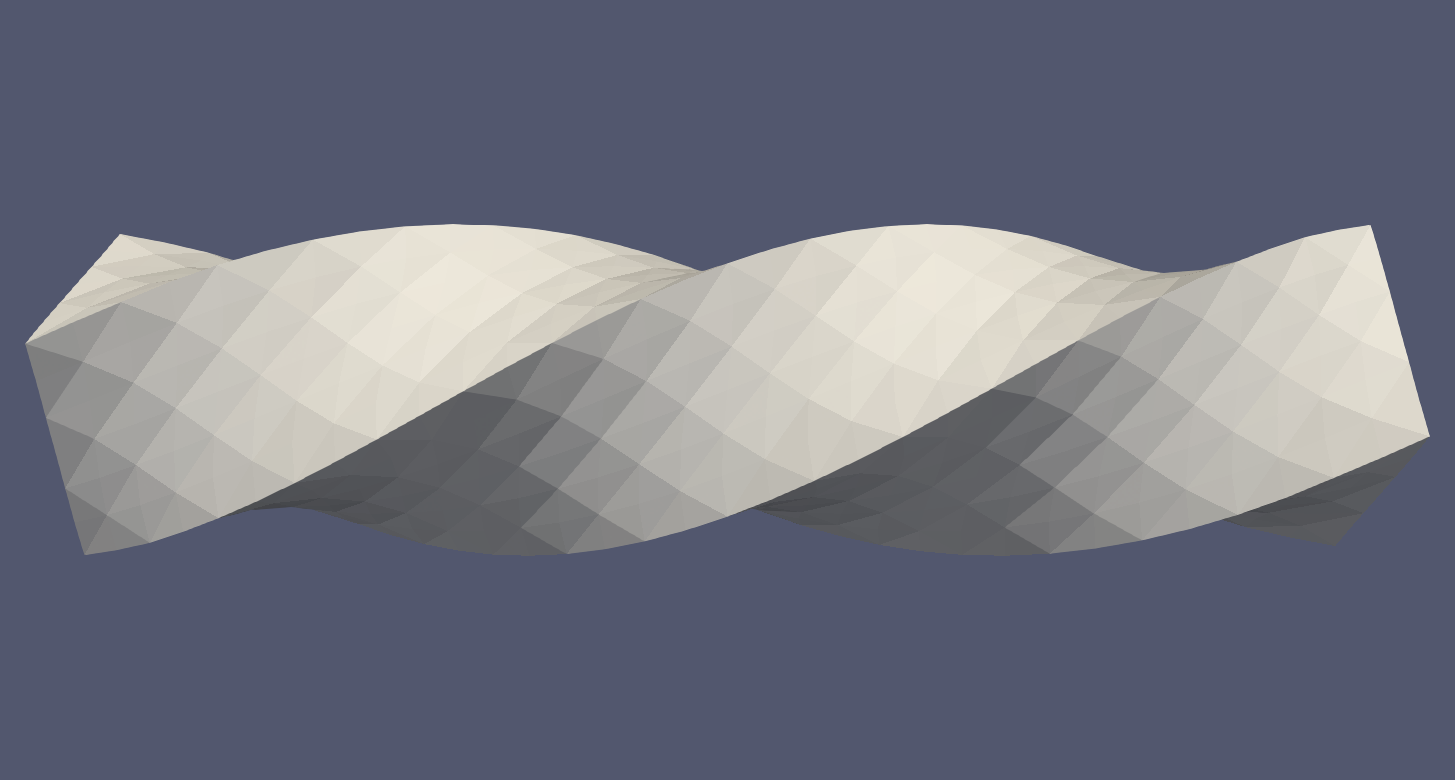
\includegraphics[width=.40\textwidth]{figures/twisted_beam.png}};
    \node[inner sep=0pt] (untwisted) at (8, 0)
        {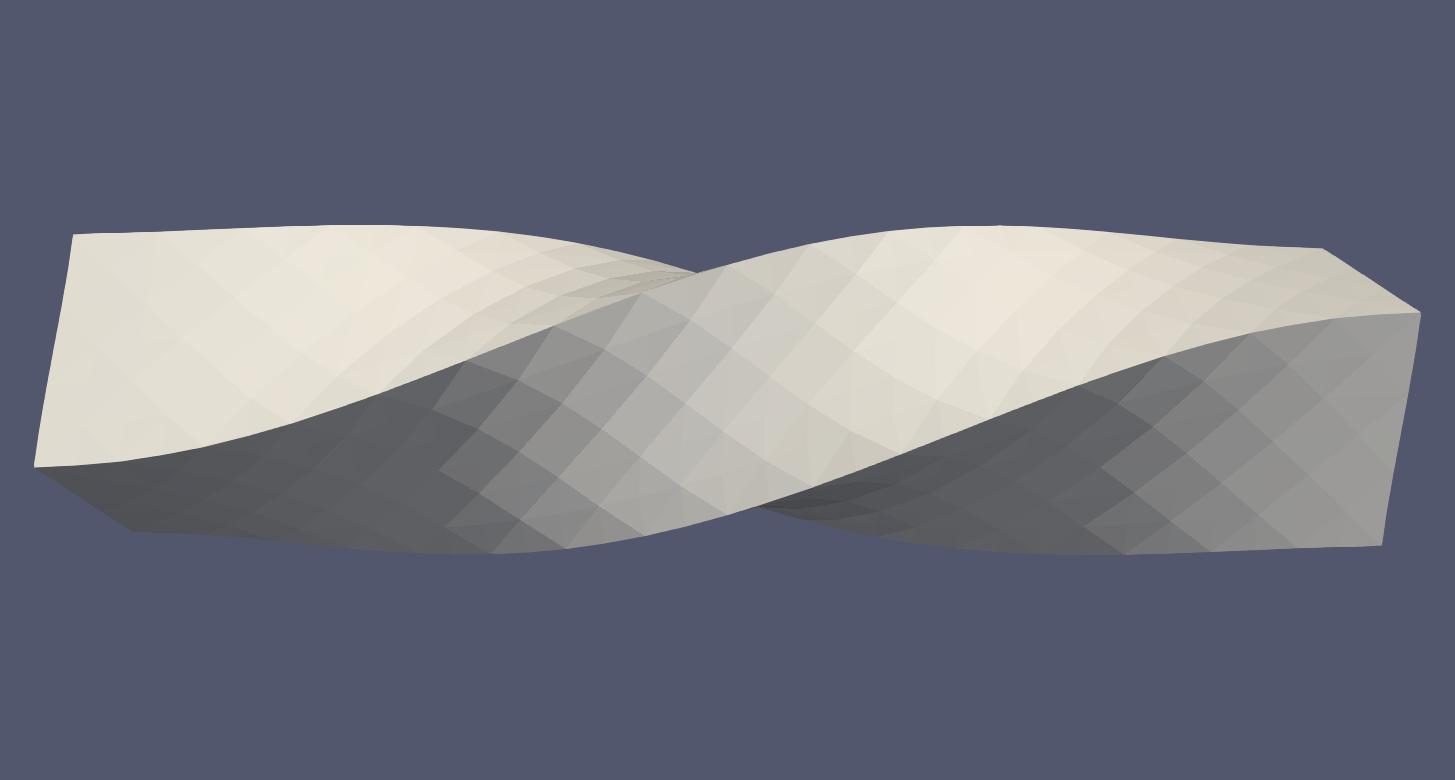
\includegraphics[width=.40\textwidth]{figures/untwisted_beam.png}};
    \node[inner sep=0pt] (further-twisted) at (8,-3.25)
        {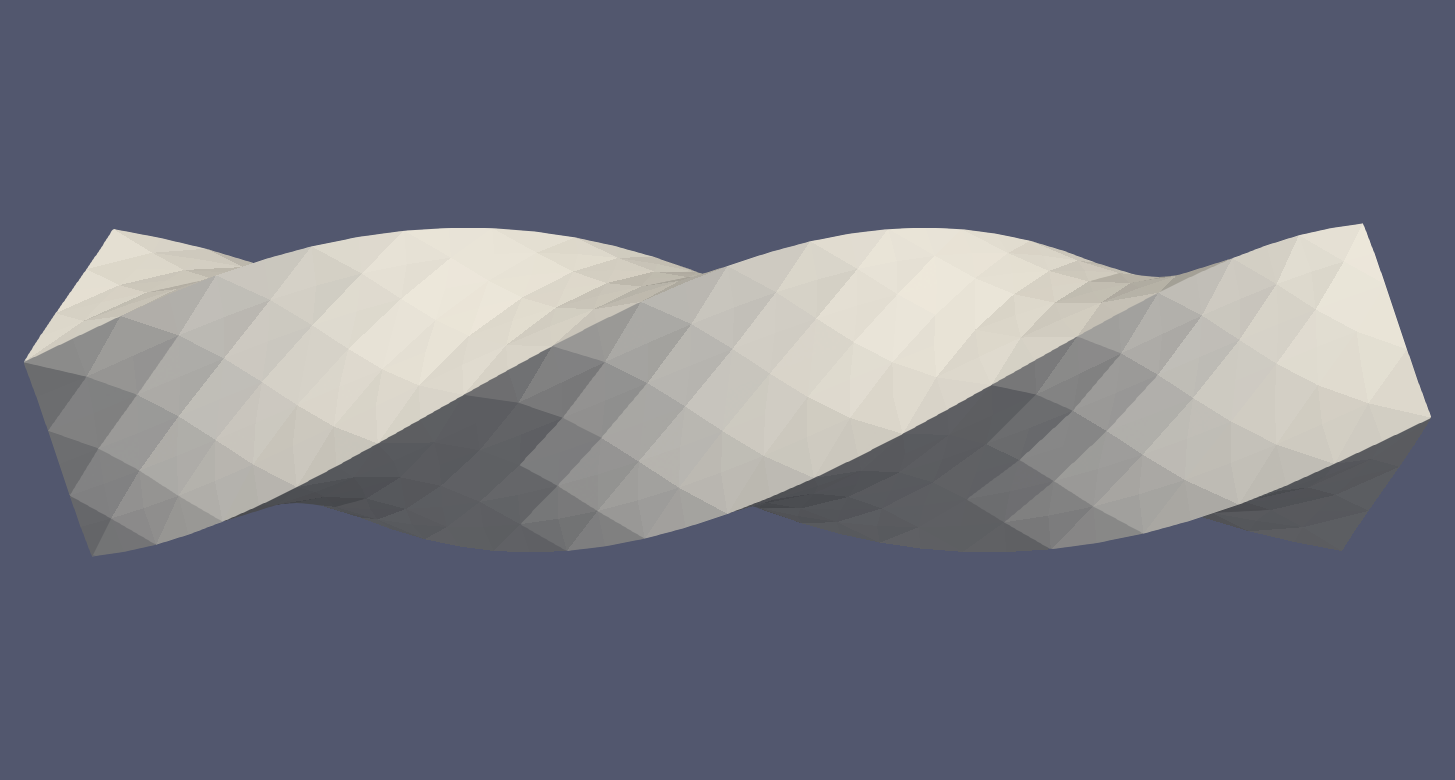
\includegraphics[width=.40\textwidth]{figures/further_twisted_beam.png}};
    \draw[->,thick] (twisted.east) -- (untwisted.west)
        node[midway,fill=white] {untwist};
    \draw[->,thick] (twisted.east) -- (further-twisted.west)
        node[midway,fill=white] {twist further};
    \end{tikzpicture}
    \caption{Visualization of the experimental settings starting from a twisted beam. The beam is either untwisted by removing position constraints at the 
    ends of the beam (top) or twisted further by rotating the anchor positions of the position constraints in-plane (bottom).}
    \label{fig:twisting-beam-setup}
\end{figure}

\noindent \textbf{Concerning PBD}\\
\noindent In contrast to XPBD and the PD-style solvers, all of which are derived from the implicit integration of the equations of motion, PBD is a geometric solver with no 
clear link to Newton's laws. As a result, the stiffness of materials simulated using PBD depends on the number of iterations and the 
chosen time step (see \cref{ss:pbd-properties}). Concomitantly, in the limit of infinite iterations and zero time step size, the material becomes infinitely stiff. 
We demonstrate this effect by example of a single solve using time steps \SI{1e-2}{\second} and \SI{1e-3}{\second} in the 
untwisting beam setting (see \cref{fig:twisting-beam-setup}) using strain constraints with stiffness \num{1e8} in \autoref{fig:strain-pbd}. Note that when using the QN 
solver, the degree to which the beam is untwisted depends on the chosen time step. In particular, the beam untwists further when the larger time step of \SI{1e-2}{\second} 
is used. In contrast, the beam is untwisted entirely to its undeformed reference configuration when using the PBD solver, regardless of the chosen time step. Of course, this 
behavior is not physically plausible. This observation and the fact that PBD can seamlessly be extended to XPBD at the cost of storing a single additional variable per 
constraint leads us to the decision to exclude PBD from the remaining experiments in this thesis and to focus on analyzing the properties of XPBD, ADMM, PD and the QN solver 
instead.

\begin{figure}
    \begin{subfigure}{0.49\textwidth}
    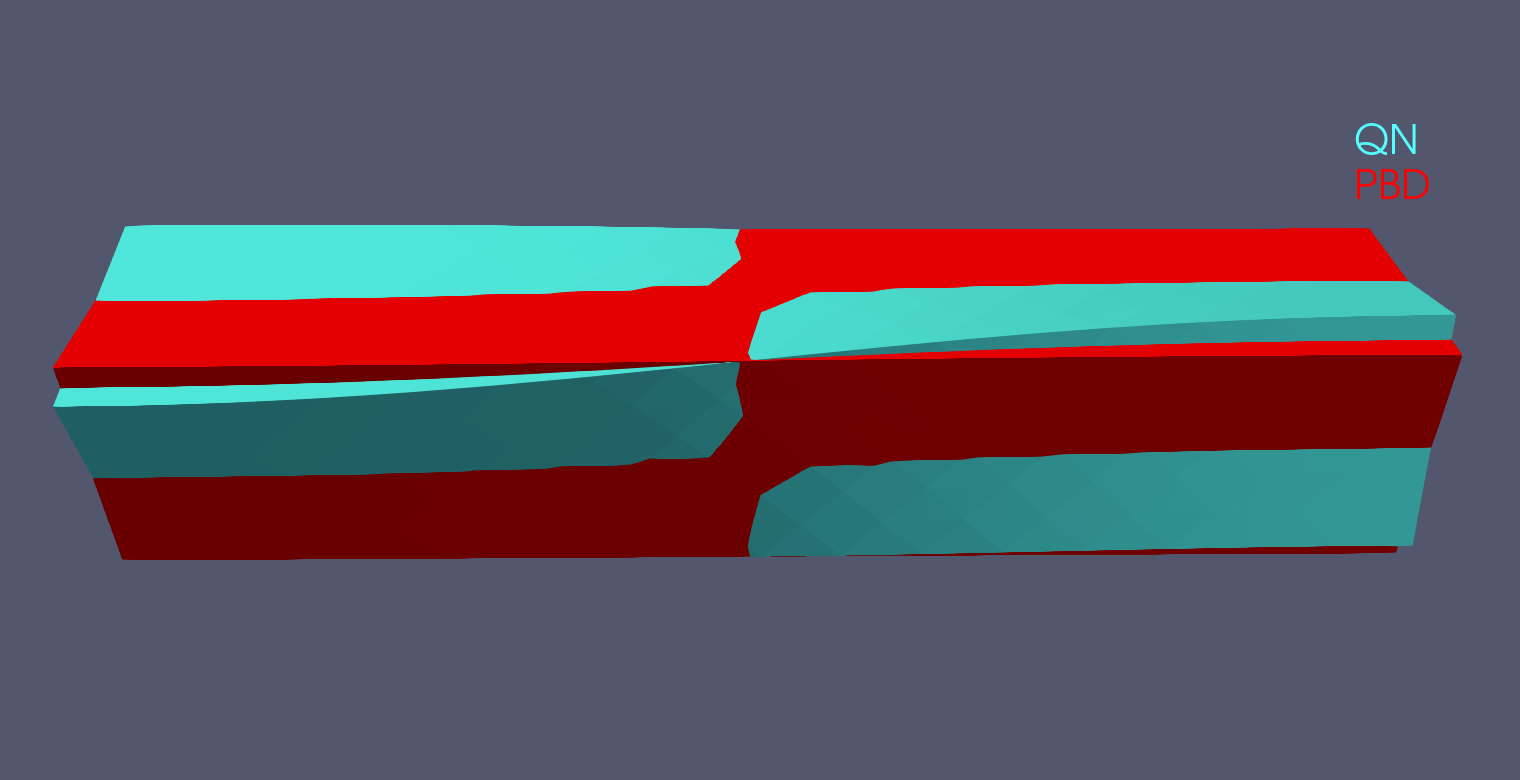
\includegraphics[width=\textwidth, trim={0 5.0cm 0 2.5cm}, clip]{figures/strain_pbd_1e-2.png}
    \subcaption{time step \SI{1e-2}{\second}}
    \end{subfigure}
    \begin{subfigure}{0.49\textwidth}
    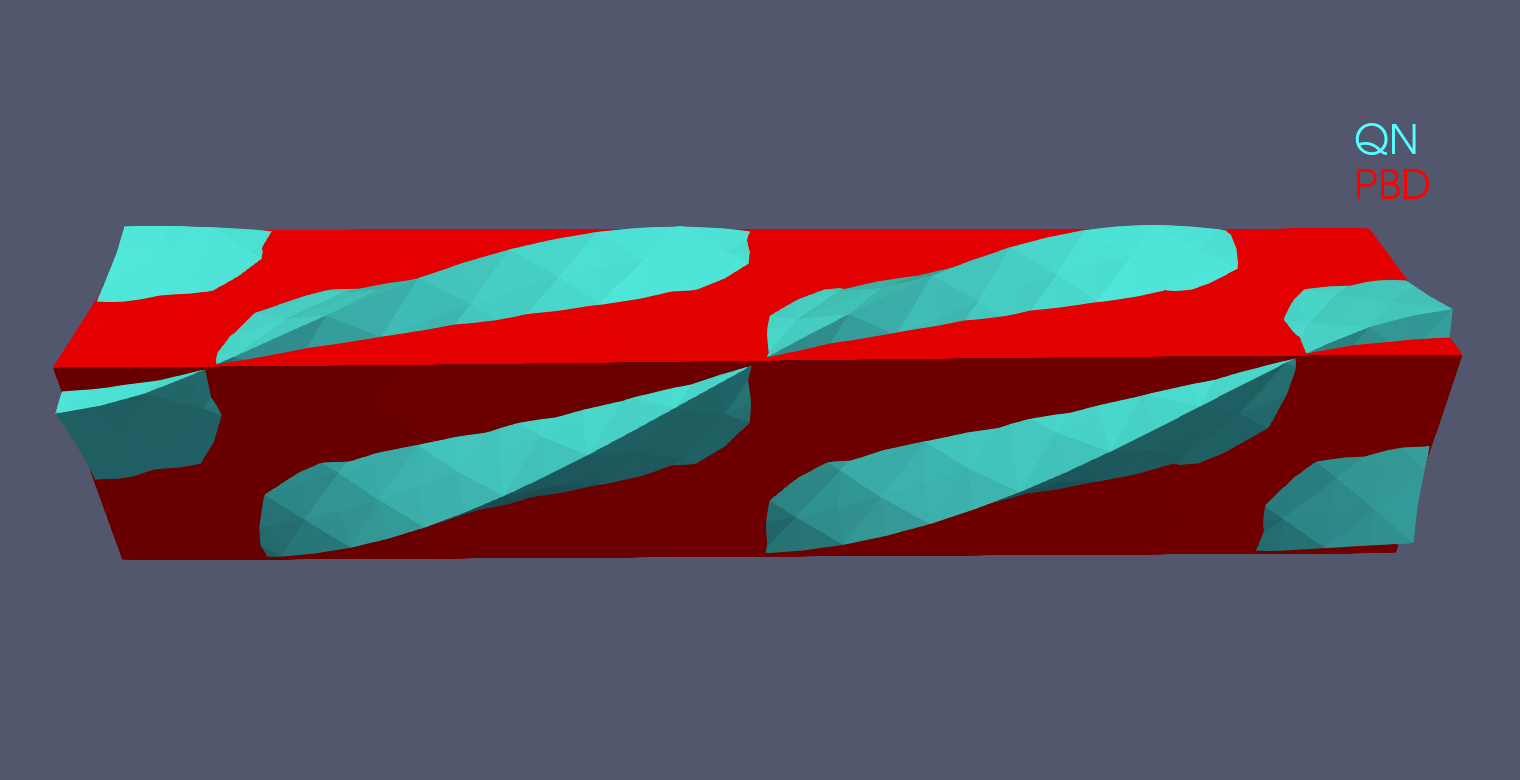
\includegraphics[width=\textwidth, trim={0 5.0cm 0 2.5cm}, clip]{figures/strain_pbd_1e-3.png}
    \subcaption{time step \SI{1e-3}{\second}}
    \end{subfigure}
    \caption{Geometries of an untwisting beam with strain constraints (stiffness \num{1e8}) after 1000 iterations of a single solve over time steps \SI{1e-2}{\second} (left) 
    and \SI{1e-3}{\second} (right) using PBD (red) and QN (cyan).}
    \label{fig:strain-pbd}
\end{figure}

\noindent \textbf{Objective function of the variational form of implicit Euler integration (\cref{eq:variational-implicit}) as a tool for analyzing convergence}\\
\noindent With the exception of PBD, all solvers discussed in the context of this thesis are based on implicit Euler integration of the equations of 
motion (\cref{ss:numerical-integration}) and aim to either approximate (XPBD) or compute exactly (PD, ADMM and QN) the implicit positions at the next time step. 
As discussed in \autoref{ss:numerical-integration}, the implicit positions can be interpreted as the positions that minimize the objective function of the variational 
form of implicit Euler integration given in \autoref{eq:variational-implicit}. To gain initial insights into the convergence behavior of the solvers, we compute 
the objective function value for the positions obtained after each iteration for each solver. The objective function is restated here for the convenience of the 
reader

\begin{equation}\label{eq:variational-implicit-copy}
    f_{\text{obj}}(\vecm{q}) \coloneq \min_{\vecm{q}} \frac{1}{2h^2} \norm{\matm{M}^{\frac{1}{2}}(\vecm{q} - \tilde{\vecm{q}})}^2_F + \sum_j \psi_j(\vecm{q}).
\end{equation}

\noindent Note again that the objective function consists of an inertial term which penalizes moving vertices away from their inertial
positions and a term that computes the constraint energies for the current configuration. The solvers are expected to decrease the objective function with each iteration 
until a value close to the minimum obtained 
by the implicit positions is obtained. By comparing the objective function values for the positions after the final iteration, the quality of the configurations different
solvers converge to can be analyzed. Further, by plotting the objective function values over the iteration number and inspecting the slope of the graphs, information about
the convergence rates of the solvers can be inferred. 

It is worth pointing out that during the discussion of the resulting figures, we consider a solver converged once the 
graph of its objective function value over the iterations is visually indistinguishable from a horizontal line. While not entirely rigorous, this is particularly appropriate 
for comparing solvers in the context of real-time applications where solver iterations that only make minor progress towards the true implicit solutions often cannot be 
afforded. Additionally, this allows setting the focus on the most important qualitative differences between solvers without getting lost in the details of when a solver can 
formally be considered converged.

\begin{figure}[h]
    \centering
    \begin{subfigure}{\textwidth}
        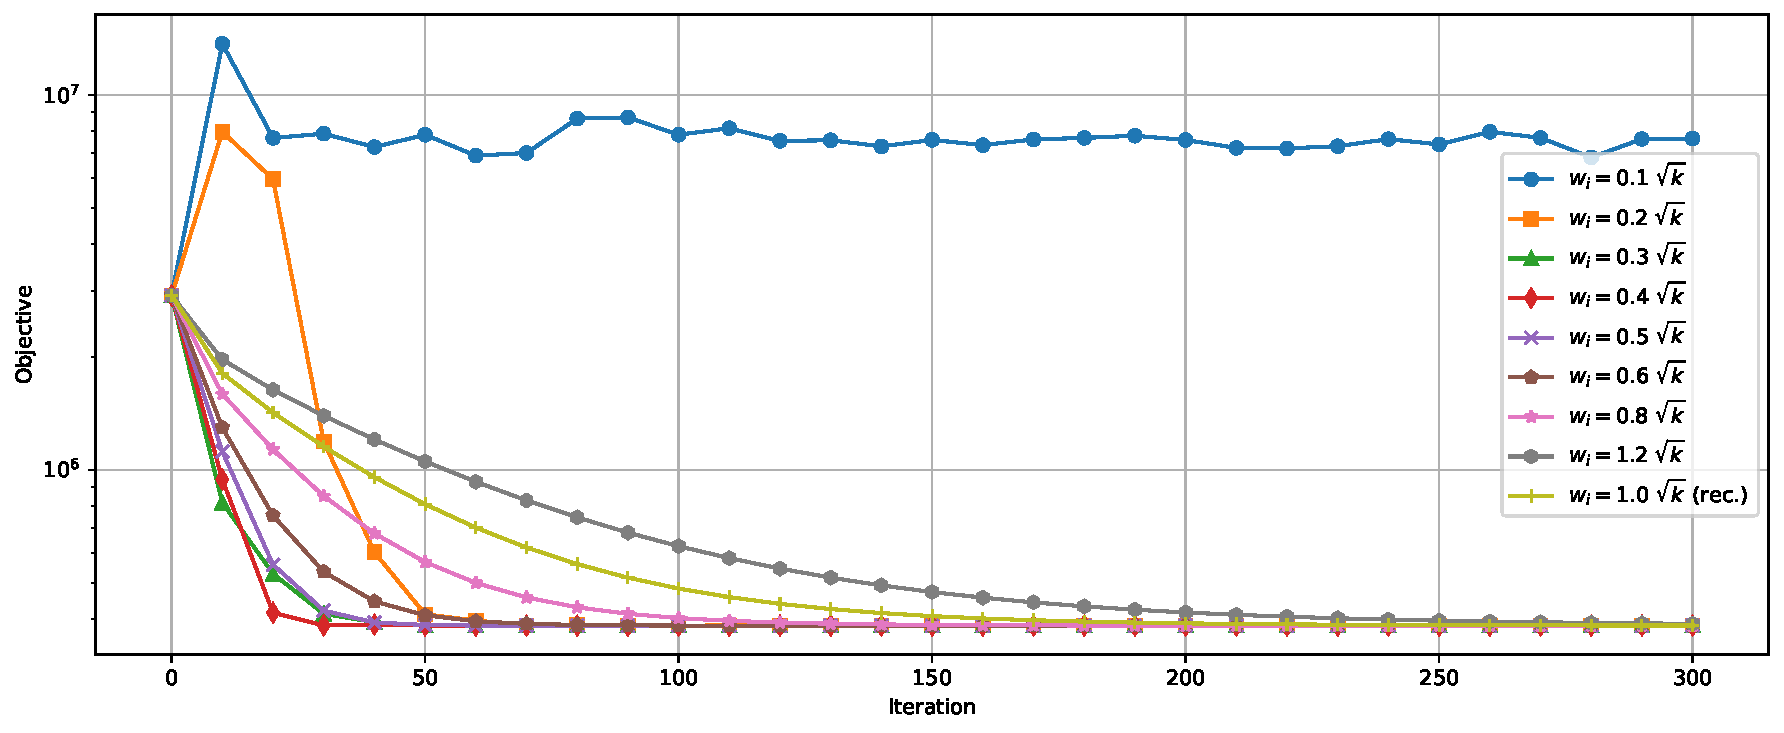
\includegraphics[width=\linewidth]{figures/strain_admm_weights_1e-2.pdf}
        \subcaption{Time step \SI{1e-2}{\second}}
    \end{subfigure}
    \begin{subfigure}{\textwidth}
        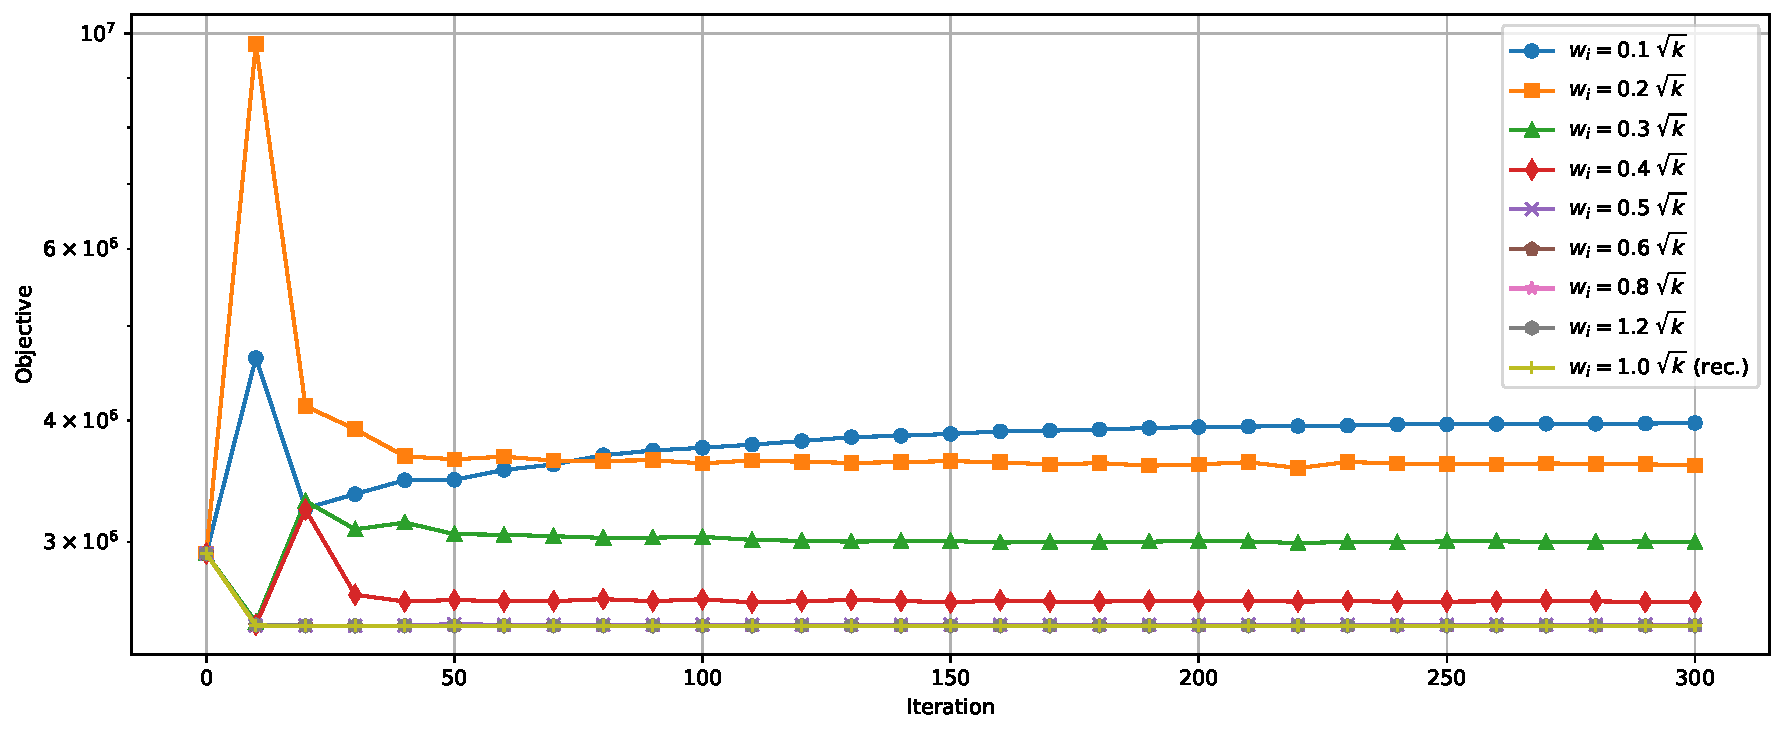
\includegraphics[width=\linewidth]{figures/strain_admm_weights_1e-3.pdf}
        \subcaption{Time step \SI{1e-3}{\second}}
    \end{subfigure}
    \caption{Values of the objective function of the variational form of implicit Euler integration (\cref{eq:variational-implicit}) over the iterations of a single 
        ADMM solve (time steps \SI{1e-2}{\second} and \SI{1e-3}{\second}) for an untwisting beam with strain constraints.}\label{fig:strain-weights-admm}
\end{figure}

\noindent \textbf{Concerning ADMM weights}\\
\noindent Before comparing solvers using the method described above, the issue of finding suitable ADMM weights needs to be discussed. For now, we restrict the discussion 
to ADMM 
weights for strain constraints. According to Overby et al.\ \cite{overby2017}, setting the weight $w_i$ of strain constraint $C_i$ with stiffness 
$k$ to $w_i = \sqrt{k}$ is a good starting point, since ADMM is almost equivalent to PD with this choice of parameters. Overby et al.\ provide experimental data for an 
untwisting beam example that suggests that reducing $w_i$ can have beneficial effects on the convergence rate of ADMM, but that the algorithm may fail to converge if 
the weights are reduced too much. In this particular example, setting $w_i = 0.5\sqrt{k}$ exhibits the best performance when examining plots of the objective 
function value over solver iterations. However, to the best of our knowledge, no method for determining the choice of $w_i$ for reliably fast convergence is available.
Thus, we manually fine-tune ADMM weights for all time steps from \SI{1e-1}{\second} to \SI{1e-4}{\second} and constraint stiffnesses from \num{1e5} to \num{1e12}.
This process reveals that ADMM weights are in fact time step dependent \textcolor{red}{(Find a justification for this when writing the part about ADMM)}. 

To see this, consider the plots of the objective function value over the number of ADMM iterations with 
different weights for time steps \SI{1e-2}{\second} and \SI{1e-3}{\second} with constraint stiffness \num{1e8} shown in \autoref{fig:strain-weights-admm}. When a time step 
of \SI{1e-2}{\second} is used (\cref{fig:strain-weights-admm} a), the ADMM solver converges to the same objective function  value for all of the weights, except for the 
lowest weight $w_i = 0.1\sqrt{k}$, where the objective function increases compared to the initial objective. The fastest convergence is achieved by setting $w_i = 0.3\sqrt{k}$ and 
$w_i = 0.4\sqrt{k}$. When picking smaller weights, the objective function value is larger than the initial objective during the first 20 iterations. Setting the weights to 
higher values than $w_i = 0.4\sqrt{k}$ leads to a slower convergence rate. However, if the time step is decreased to \SI{1e-3}{\second} (\cref{fig:strain-weights-admm} b), 
weights higher than $w_i = 0.4\sqrt{k}$ achieve a better convergence rate and converge to configurations that achieve lower objective function values than weights lower than 
or equal to $w_i = 0.4\sqrt{k}$. In particular, ADMM converges to a solution whose objective function value is higher than the initial objective when using $w_i = 0.2\sqrt{k}$ and 
$w_i = 0.3\sqrt{k}$. Thus, $w_i = 0.3\sqrt{k}$ is an excellent weight for time step \SI{1e-2}{\second}, while it is unsuitable for time step \SI{1e-3}{\second}. Overall, it can be 
seen that more aggressive reductions of the ADMM weights without jeopardizing convergence are possible when a larger time step is used. Qualitatively equivalent results 
can be observed for other stiffness values. Note that this time step dependence makes finding suitable ADMM weights incredibly tedious: For each material model, weights 
need to be manually determined for each combination of time step size and material stiffness. From now on, experiments involving the ADMM solver use manually fine-tuned 
weights for optimal performance.

\begin{figure}[h]
    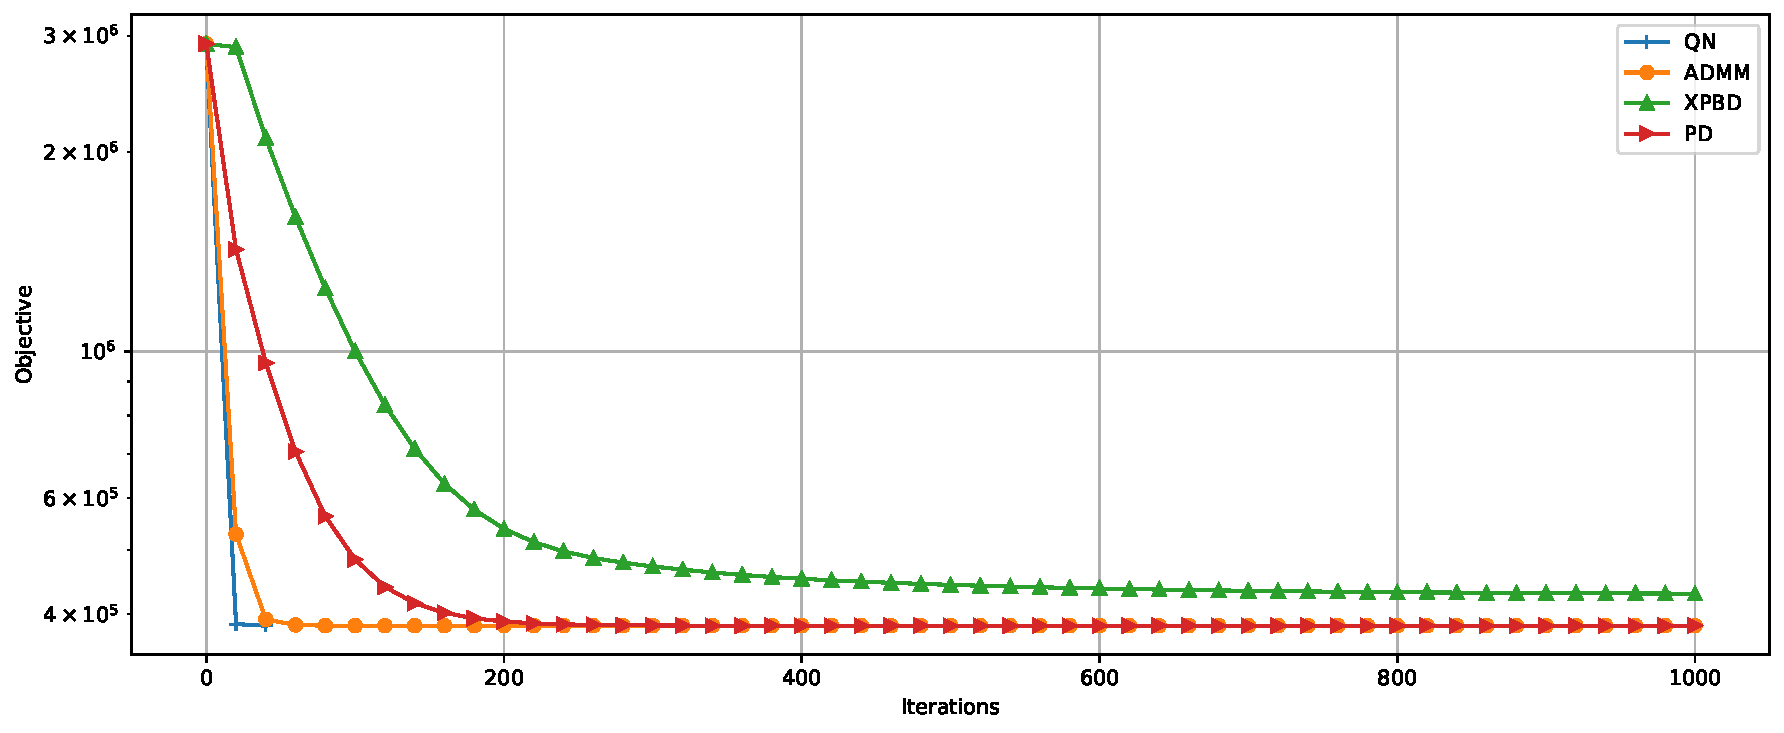
\includegraphics[width=\textwidth]{figures/strain_beam_untwist_objectives.pdf}
    \caption{Values of the objective function of the variational form of implicit Euler integration (\cref{eq:variational-implicit}) over the iterations of a single solve (time step 
        \SI{1e-2}{\second}) for an untwisting beam using strain constraints}
    \label{fig:strain-beam-untwist-objectives}
\end{figure}

\noindent \textbf{Analyzing convergence behavior of solvers}\\ 
\noindent In \autoref{fig:strain-beam-untwist-objectives}, the objective function values are plotted for an untwisting beam whose material is modelled using strain constraints 
\cite{bouaziz2014}. The graph shows that each of the solvers indeed mostly decreases the objective function from iteration 
to iteration until it converges towards a final configuration after a sufficient number of iterations. ADMM, PD and QN converge to configurations that 
yield roughly the same objective function value whereas the value obtained after 1000 XPBD iterations is still slightly larger. QN and ADMM converge after roughly 40 
and 60 iterations, whereas PD and XPBD converge after upwards of 260 and 1000 iterations, respectively. In order to quantify the progress that other solvers
achieve during the number of iterations it takes each of the solvers to converge, we compute relative errors after 40 (QN), 60 (ADMM), 260 (PD) and 1000 (XPBD)
iterations. The relative error is given by 

\begin{equation}\label{eq:rel-error}
    \frac{f_{\text{obj}}(\vecm{q}_k) - f_{\text{obj}}(\vecm{q}^*)}{f_{\text{obj}}(\vecm{q}_0) - f_{\text{obj}}(\vecm{q}^*)},
\end{equation}

\noindent where $\vecm{q}_k$ are the positions after iteration $k$ and $\vecm{q}^*$ are the positions for which the minimal objective function value is achieved.
The relative errors are shown in \autoref{fig:rel-errors}. Note that the relative error of ADMM is only 0.4 \% by the time QN has converged, while the errors 
achieved by PD and XPBD are still substantial. Additionally, even after a 1000 iterations, XPBD's relative error is only at 1.8 \%.

\begin{table}[h]
\centering
\begin{tabular}{ |r||c|c|c|c| } 
 \hline
 & QN & ADMM & PD & XPBD\\
 \hline
 \hline
    40 iterations (QN) & 0.0 & 0.4 & 22.7 & 67.8 \\ 
    60 iterations (ADMM) & 0.0 & 0.0 & 12.6 & 47.8 \\
    260 iterations (PD) & 0.0 & 0.0 & 0.0 & 4.0 \\
    1000 iterations (XPBD) & 0.0 & 0.0 & 0.0 & 1.8 \\ 
 \hline
\end{tabular}
\caption{Relative errors (see \cref{eq:rel-error}) in \% achieved by solvers after 40, 60, 260 and 1000 iterations for the untwisting beam experiment from 
\autoref{fig:strain-beam-untwist-objectives}.}
\label{fig:rel-errors}
\end{table}

The data suggests that ADMM, PD and QN converge towards a solution that is closer to the true implicit positions at the next time step than XPBD. This is expected, 
as XPBD only approximates a solution to the implicit equations of motion due to the simplifying assumptions made during its derivation (\cref{ss:xpbd-properties}).
Due to the second assumption (\cref{eq:xpbd-assumption-2}) in particular, there is no penalty for moving vertex positions away from their inertial positions during 
the XPBD constraint projections (see \cref{ss:xpbd-properties}), even though it increases the objective function. Additionally,
it is not clear whether the Gauss-Seidel solver at the core of XPBD is able to minimize the constraint energies sufficiently via local constraint projections only.
Since constraints are projected independently one-by-one, later constraint projections can undo some of the work achieved by previous projections. Bouaziz et al.\ 
\cite{bouaziz2014} describe this phenomenon as an oscillation between different constraints. On the other hand ADMM, PD and QN aim to solve the implicit equations of motion exactly. The difference in the rate of convergence between ADMM and PD goes in line 
with experimental data provided by Overby et al.\ \cite{overby2017}. There, the authors show that ADMM with a weight of $\sqrt{k}$, where $k$ is the stiffness of the 
strain constraints, is almost equivalent to PD and that the convergence rate can often be improved by fine-tuning the weight \textcolor{red}{(Why exactly is reducing the 
weight favorable? I don't know \ldots)}. Similarly, the faster convergence rate of QN compared to PD is expected in light of the observation that PD is a quasi-Newton method 
with constant Hessian approximation (see \cite{liu2017}, \cref{ss:pd-quasi-newton}). The QN solver augments the PD solver with a line-search algorithm and LBFGS-updates to 
the constant Hessian approximation from PD that take into account curvature information from previous iterations in order to better approximate the true Hessian matrix. Both
of these measures help improve the convergence rate of QN in comparison to PD. Again, this is in line with results presented by Liu et al.\ \cite{liu2017}. The comparably
slow convergence rate of XPBD could again be explained by the simplifying assumptions made during the XPBD derivation and the aforementioned oscillations of Gauss-Seidel
solvers. 

\begin{figure}[h]
    \centering
    \begin{subfigure}{\textwidth}
        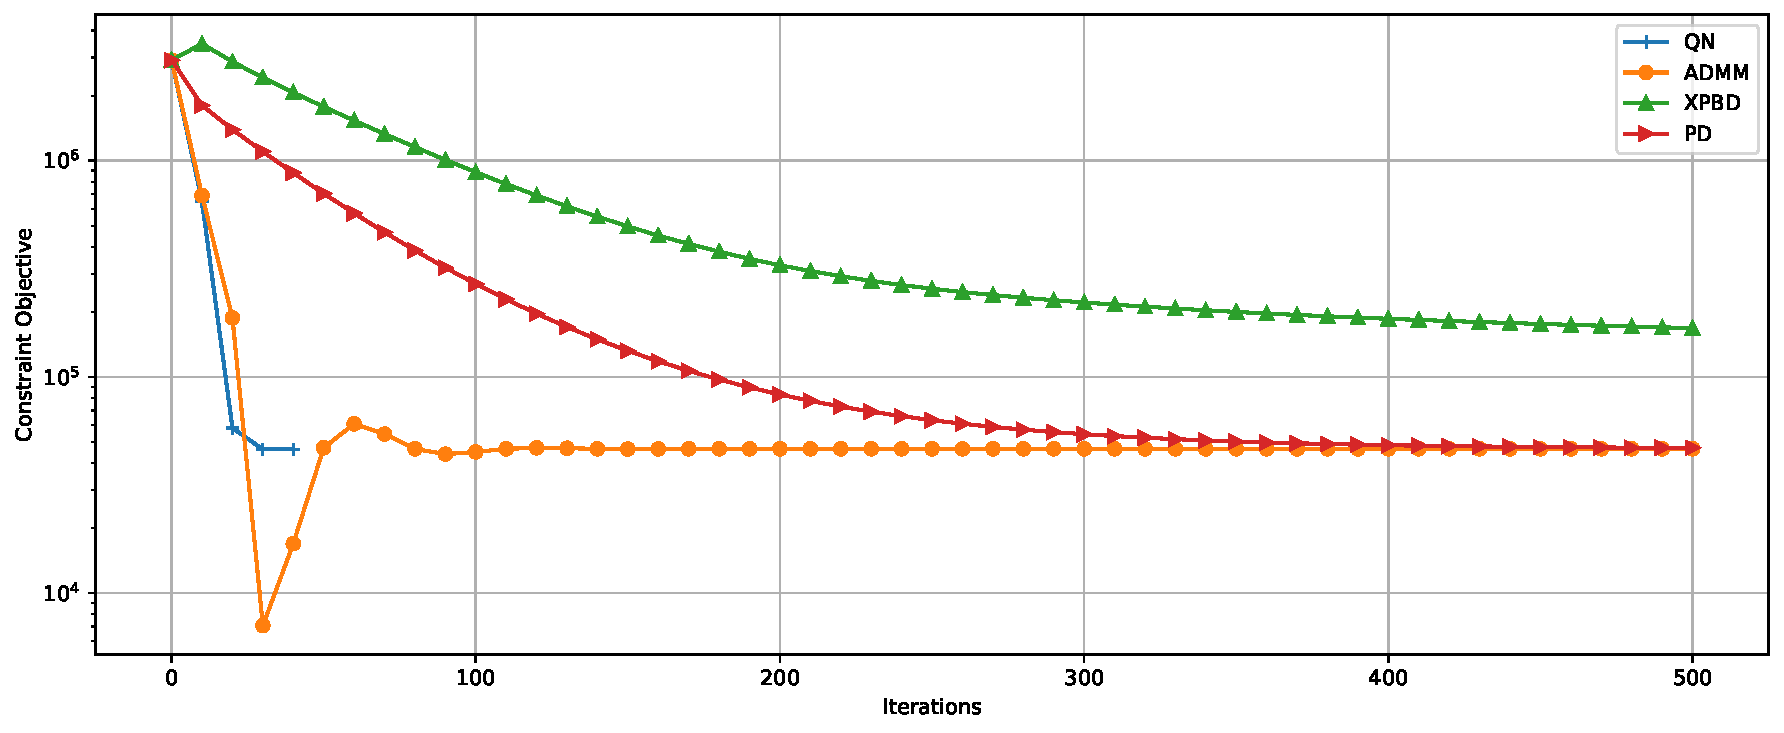
\includegraphics[width=\linewidth]{figures/strain_beam_untwist_constraintObjectives.pdf}
    \end{subfigure}
    \begin{subfigure}{\textwidth}
        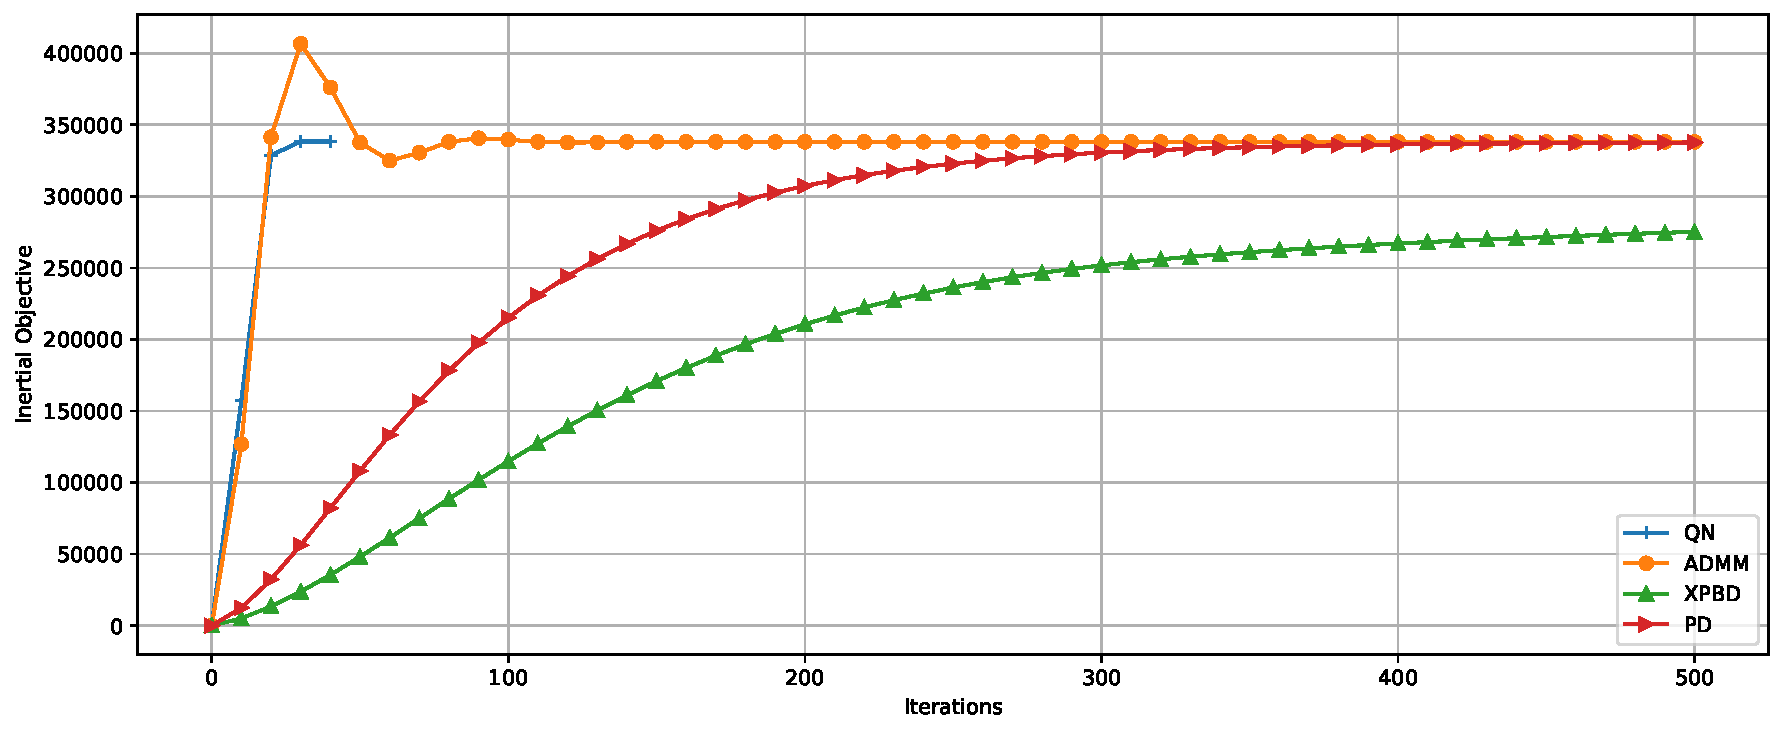
\includegraphics[width=\linewidth]{figures/strain_beam_untwist_inertialObjectives.pdf}
    \end{subfigure}
    \caption{Values of the constraint (top) and inertial (bottom) terms of the objective function of the variational form of implicit Euler integration 
        (\cref{eq:variational-implicit}) over the iterations of a single solve (time step \SI{1e-2}{\second}) for an untwisting beam with strain constraints.}
    \label{fig:strain-beam-untwist-objectives-split}
\end{figure}

To better understand the main factor for XPBD's unfavorable convergence properties, it is helpful to plot the inertial and the constraint terms of the objective function 
separately. The resulting plots for the same untwisting beam experiment are shown in \autoref{fig:strain-beam-untwist-objectives-split}. 
We focus on the first 500 iterations in order to gain clearer insights into the behavior of the solver during earlier iterations, since that is more relevant for 
real-time applications. First, it is evident that the constraint term dominates the objective function value for each solver during most of the iterations before 
convergence is achieved. While each solver mostly decreases the constraint term with an increasing number of iterations, the inertial term is mostly increased. 
ADMM, PD and QN converge to configurations with roughly the same inertial and constraint terms. However, at its converged state, the constraint term of the XPBD 
solver is higher than its counterparts from the PD-style solvers, whereas the opposite is observed for the inertial term. 

As discussed in \autoref{ss:variational-implicit-euler}, the weighting between the inertial term and the constraint term depends on the time step, the particle masses 
and the material stiffnesses. The results suggest that with a time step of \SI{1e-2}{\second} and a constraint stiffness of \num{1e8}, the constraint energies can be 
decreased significantly until the cost of moving particles away from their inertial positions becomes too high. Since the inertial term at the converged XPBD state 
is in fact lower than the inertial terms achieved by PD-style solvers, it is evident that the reason for the higher objective function of XPBD is the constraint term.
Thus, XPBD's inferior performance in this experiment is likely due to an inability to decrease the constraint energies sufficiently. It is natural to assume that this 
is in part a consequence of the oscillations resulting from the iterative Gauss-Seidel solver used in XPBD. However, it is worth pointing out again that XPBD does not 
solve the implicit equations of motion exactly due to the simplifying XPBD assumptions. Even if \autoref{eq:xpbd-simplified-lse} were to be solved with a global solver,
it is not clear whether the constraint term would be decreased further than it is using the Gauss-Seidel solver. 

The fact that the inertial term achieved by the 
converged state of the XPBD solver is smaller than the final inertial term of the other solvers is surprising considering that the inertial positions do not appear 
in the update equations of XPBD (see \cref{ss:xpbd-properties}). On the other hand, the only factor driving particles away from their inertial positions in the untwisting 
beam experiment are the elastic energies due to the deformation of the beam. One possible explanation for the low inertial term for XPBD might be that the particles do 
not move far away from their inertial positions simply because the XPBD constraint solver is not as successful at minimizing the constraint energies. Lastly, the 
penalty for moving particles from their inertial positions is quite low for PD-style solvers if a time step as large as \SI{1e-2}{\second} is used. However, the 
inertial term achieved by XPBD remains smaller than its counterparts, even if the timestep is decreased.

The fact that the constraint term is higher for the final state of the XPBD solver is also perceptible when comparing its geometry with the final geometries computed 
by PD-style solvers. The geometries achieved after 1000 XPBD and QN iterations are shown in \autoref{fig:strain-beam-untwist-geometries} a. 
The corresponding geometries for PD and ADMM are ommitted since they are visually indistinguishable from the geometry computed by the QN solver. The image shows 
that the QN solver untwists the beam 
further towards its undeformed rest configuration than XPBD. Since the constraint energies obtain a minimum at the reference configuration, this is in line 
with the observation that QN is more successful than XPBD at reducing the constraint term of the objective function.

In the context of real-time applications, the number of solver iterations is often capped in order to ensure that the computations fit into the time budget allocated 
for the simulation of the next frame. A closer look at \autoref{fig:strain-beam-untwist-objectives-split} shows that none of the solvers achieves the 
minimal objective function value during the first 10 iterations. After 10 iterations, the QN solver has reduced the objective function the most, followed 
by ADMM, PD and XPBD. In order to gain a better understanding of the effects caused by terminating solvers before the objective function is minimized, we take a 
closer look at the geometries that the XPBD, PD and ADMM solvers arrive at after 10 solver iterations in \autoref{fig:strain-beam-untwist-geometries} b-d. The 
corresponding QN geometry is given as a reference in each panel. \autoref{fig:strain-beam-untwist-geometries} b-d shows that the solvers untwist the beam to 
different extents after the first 10 solver iterations. The QN geometry gets closest to the beam's reference configuration, again followed by ADMM, PD and, lastly, 
XPBD. Note that the degree to which solvers untwist the beam goes hand-in-hand with the extent to which they minimize the objective function and particularly its 
constraint term. 

\begin{figure}
    \centering
    \begin{subfigure}{0.49\textwidth}
        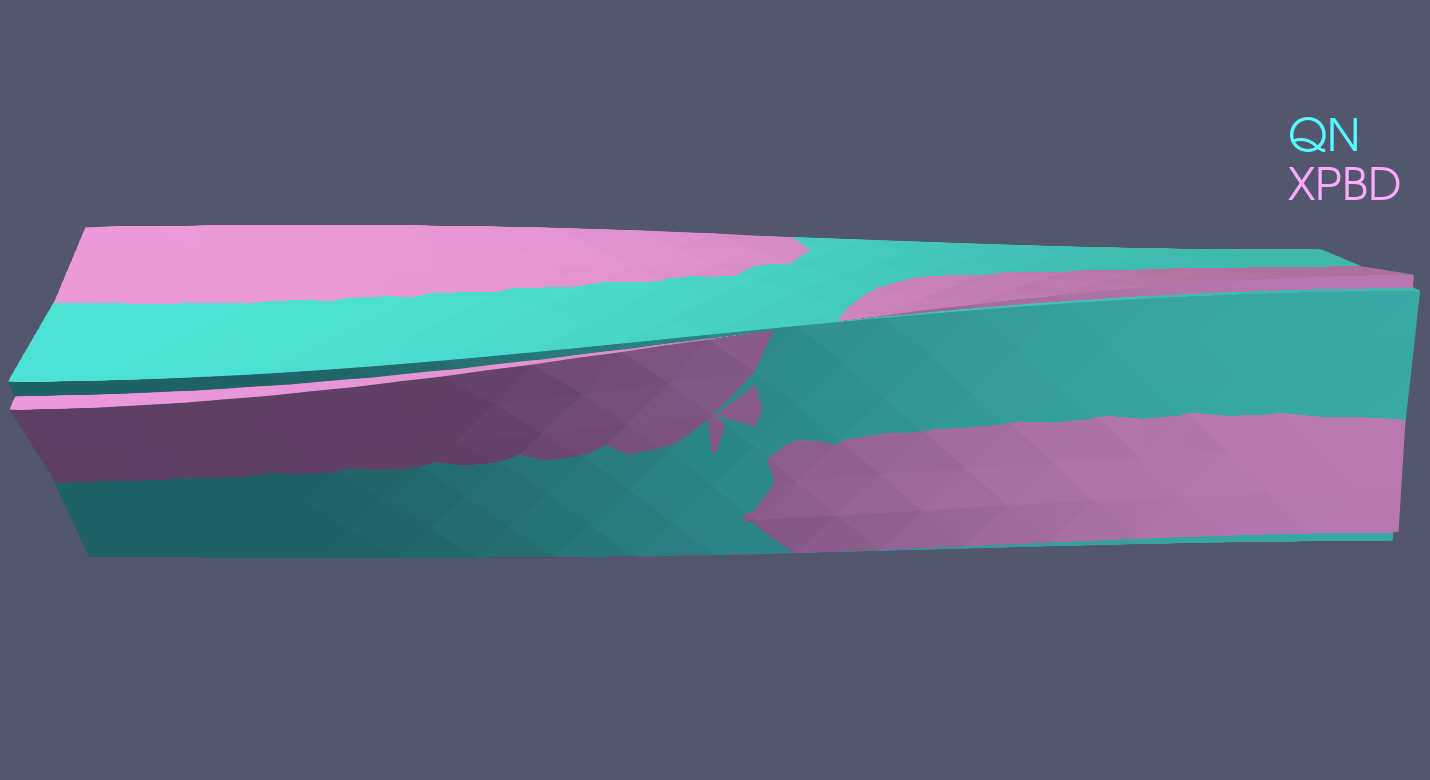
\includegraphics[width=\textwidth, trim={0 5.0cm 0 2.5cm}, clip]{figures/strain_beam_untwist_QN_vs_XPBD.png}
        \subcaption{QN and XPBD after 1000 iterations}
    \end{subfigure}
    \hspace{0.001\textwidth}
    \begin{subfigure}{0.49\textwidth}
        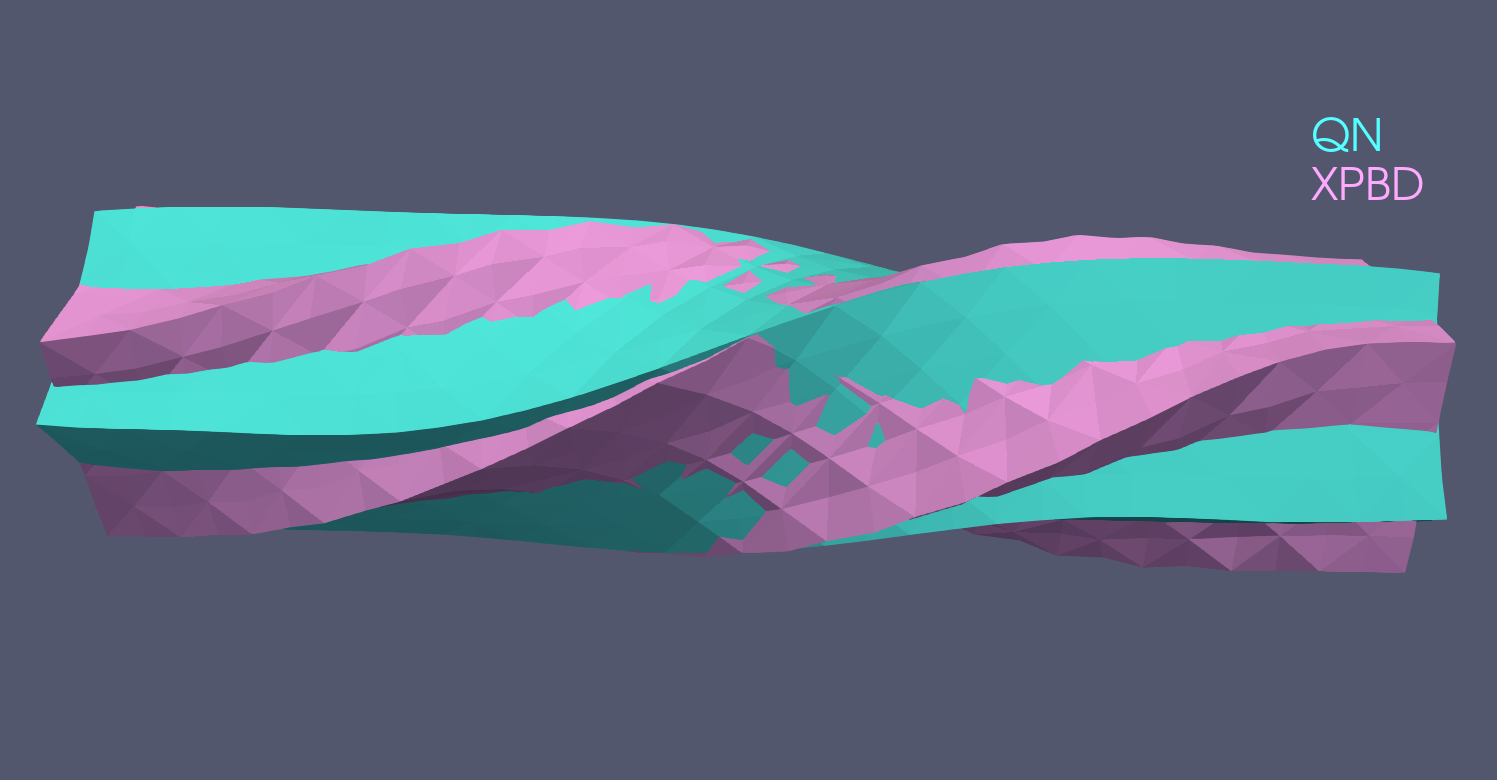
\includegraphics[width=\textwidth, trim={0 4.5cm 0 2.15cm}, clip]{figures/strain_beam_untwist_QN_vs_XPBD_10_iterations.png}
        \subcaption{QN and XPBD after 10 iterations}
    \end{subfigure}
    \par\medskip
    \begin{subfigure}{0.49\textwidth}
        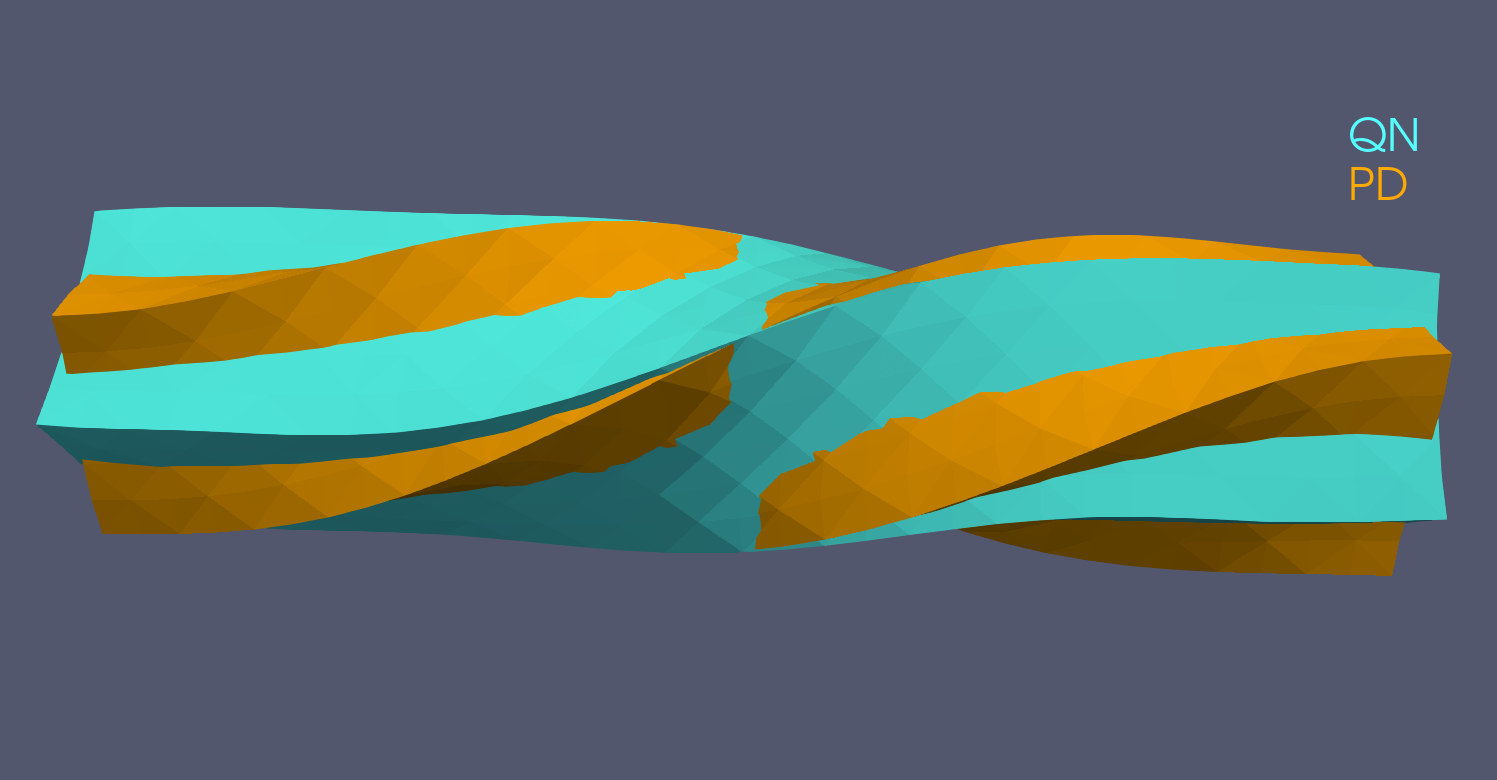
\includegraphics[width=\textwidth, trim={0 4.5cm 0 2.15cm}, clip]{figures/strain_beam_untwist_QN_vs_PD_10_iterations.png}
        \subcaption{QN and PD after 10 iterations}
    \end{subfigure}
    \hspace{0.001\textwidth}
    \begin{subfigure}{0.49\textwidth}
        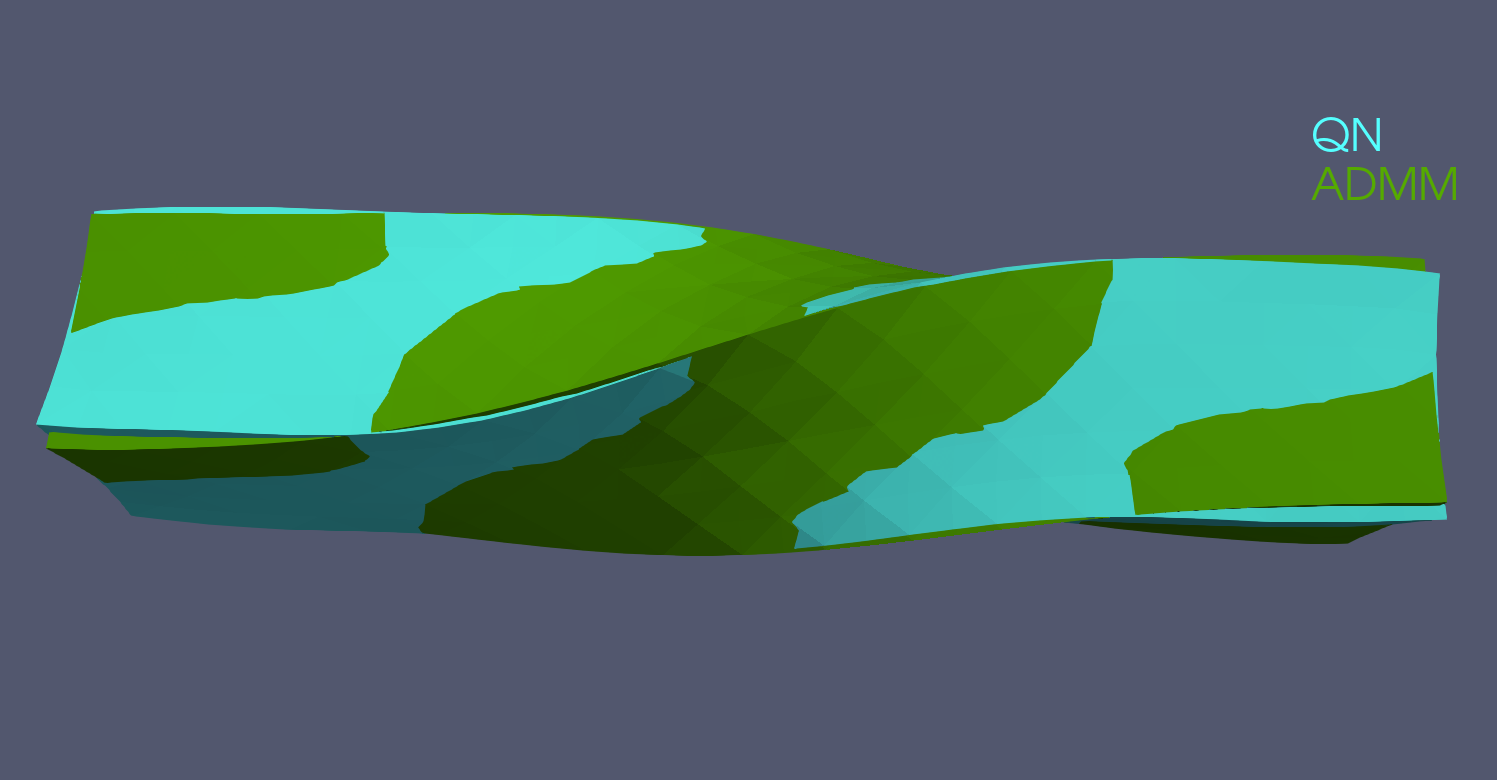
\includegraphics[width=\textwidth, trim={0 4.5cm 0 2.15cm}, clip]{figures/strain_beam_untwist_QN_vs_ADMM_10_iterations.png}
        \subcaption{QN and ADMM after 10 iterations}
    \end{subfigure}
    \caption{Geometries of an untwisting beam with strain constraints after 10 and 1000 iterations of a single solve over a time step of \SI{1e-2}{\second} using 
        XPBD (pink), PD (orange), ADMM (gree) and QN (cyan) solvers.}
    \label{fig:strain-beam-untwist-geometries}
\end{figure}

Again, the relation between untwisting the beam and reducing the constraint term of the objective function is expected in the light of the fact that the constraint 
term is minimized in the reference configuration of the beam. The results suggest that some of the constraint energy stored in the deformed beam is converted into kinetic 
energy by untwisting the beam during each solver iteration. Additionally, solvers with a faster convergence rate appear to be able to convert a larger share of the elastic 
energy into kinetic energy during a single iteration. To confirm this, we have plotted the kinetic energies of the configurations after each iteration in 
\autoref{fig:strain-beam_untwist-kinetic-energies}. The particle velocities $\vecm{v}_k$ required for the computation of the kinetic energy after iteration $k$ are 
computed using Verlet integration via $\vecm{v}_k = (\vecm{q}_k - \vecm{q}_{\text{initial}}) / h$, where $\vecm{q}_k$ are the positions after iteration $k$, 
$\vecm{q}_{\text{initial}}$ are the initial positions and $h$ is the timestep. Indeed, \autoref{fig:strain-beam_untwist-kinetic-energies} shows that the kinetic 
energy increases with the number of iterations for all solvers. Additionally, the QN solver achieves the highest kinetic energy after 10 iterations, followed by ADMM, PD 
and XPBD. As a consequence, terminating the solvers after a small number of iterations can cause the motion of simulated bodies to appear slowed down. This effect is more 
noticable for solvers that have inferior convergence properties, such as PD and XPBD.

Closer inspection of \autoref{fig:strain-beam-untwist-geometries} b shows that the XPBD geometry is noticably rugged compared to the geometries of the PD-solvers, which 
appear mostly smooth at the surface. This matches the observation that the constraint objective achieved after 10 XPBD iterations is larger than the initial constraint 
objective in \autoref{fig:strain-beam-untwist-objectives-split}. While it is difficult to verify, it is natural to assume that this effect is caused by oscillations 
of the Gauss-Seidel solver at the core of XPBD, since it does not appear for solvers that have a global optimization step. 

\begin{figure}
    \centering
    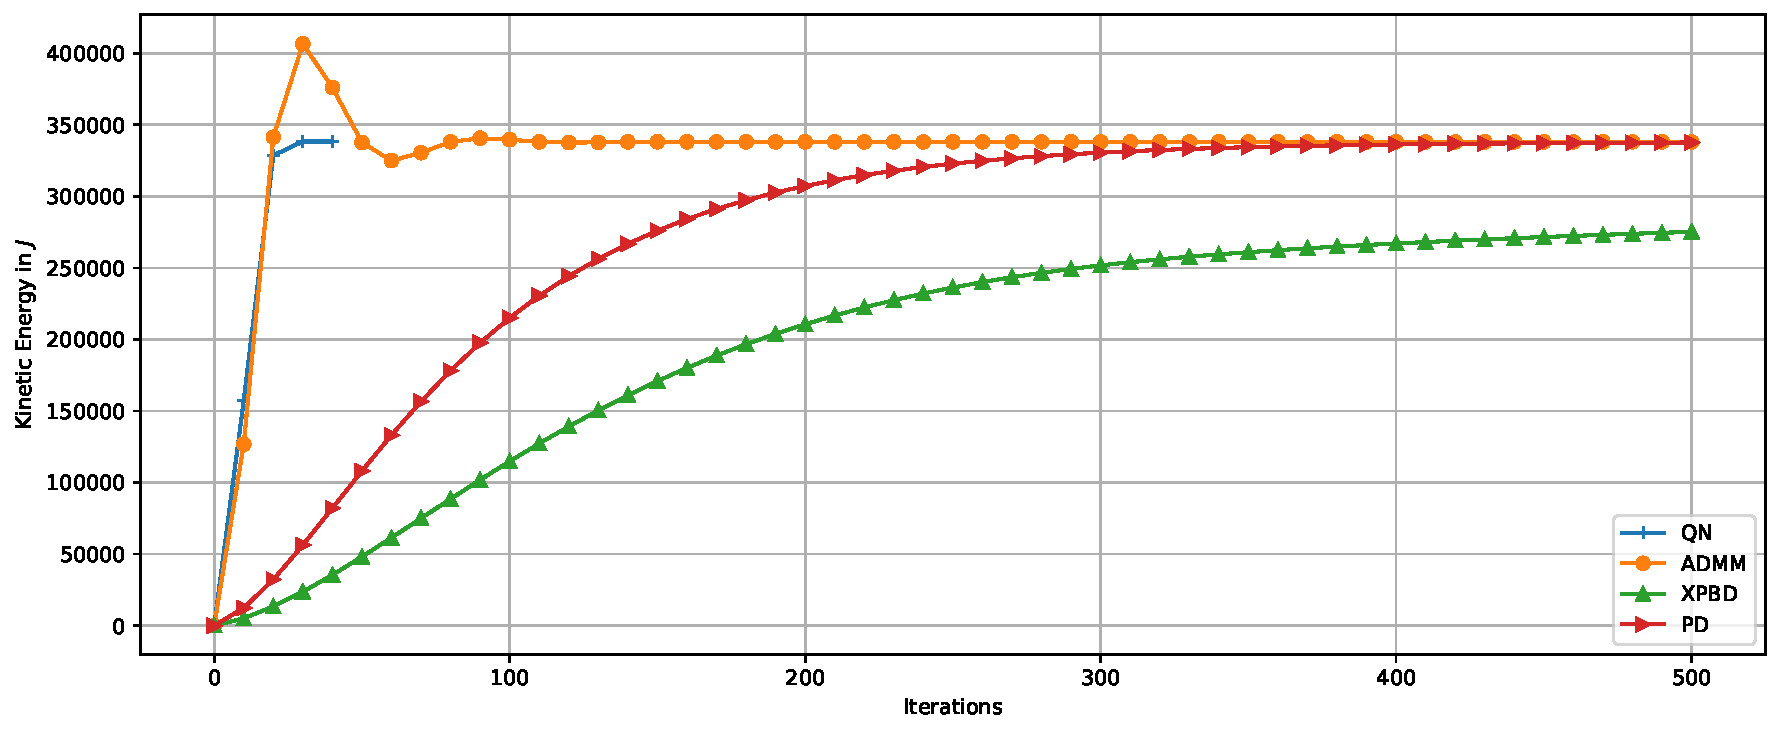
\includegraphics[width=\textwidth]{figures/strain_beam_untwist_kinetic_energies.pdf}
    \caption{Kinetic energies over the iterations of a single solve (time step \SI{1e-2}{\second}) for an untwisting beam with strain constraints. The velocities 
    are computed via Verlet integration.}
    \label{fig:strain-beam_untwist-kinetic-energies}
\end{figure}

\autoref{fig:strain-beam-untwist-objectives} shows data for time step \SI{1e-2}{\second} and constraint stiffness \num{1e8}. While the results are qualitatively 
the same for a wide range of time steps and stiffness values, noticable differences arise when a combination of large time steps and large stiffness values is used.

In order to take into account the computational cost of the iterations for different solvers, the objective function values are plotted again over the accumulated
iteration durations in \autoref{fig:strain-beam-untwist-objectives-time} \textcolor{red}{(this should be done for beams of different sizes to show how the simulation
time grows for each solver!)}. However, the provided iteration durations should be treated as a rough indication of the 
computational costs of different solvers since no effort has been put into profiling or speeding up the computations by providing a multithreaded 
implementation. While QN iterations appear to be almost twice as computationally expensive as the iterations 
for the other solvers, the costs associated with a single iteration are on average very simular. Note that 500 iterations of XPBD, ADMM and PD 
take roughly 2 seconds each. Due to the similar computational costs per iterations, the conclusions that can be drawn from \autoref{fig:strain-beam-untwist-objectives-time}
are similar to what was discussed for \autoref{fig:strain-beam-untwist-objectives}: ADMM and QN converge in a shorter amount of time than XPBD and PD, but ADMM and PD
appear in a more favorable light compared to QN due to faster iterations.

\begin{figure}[h]
    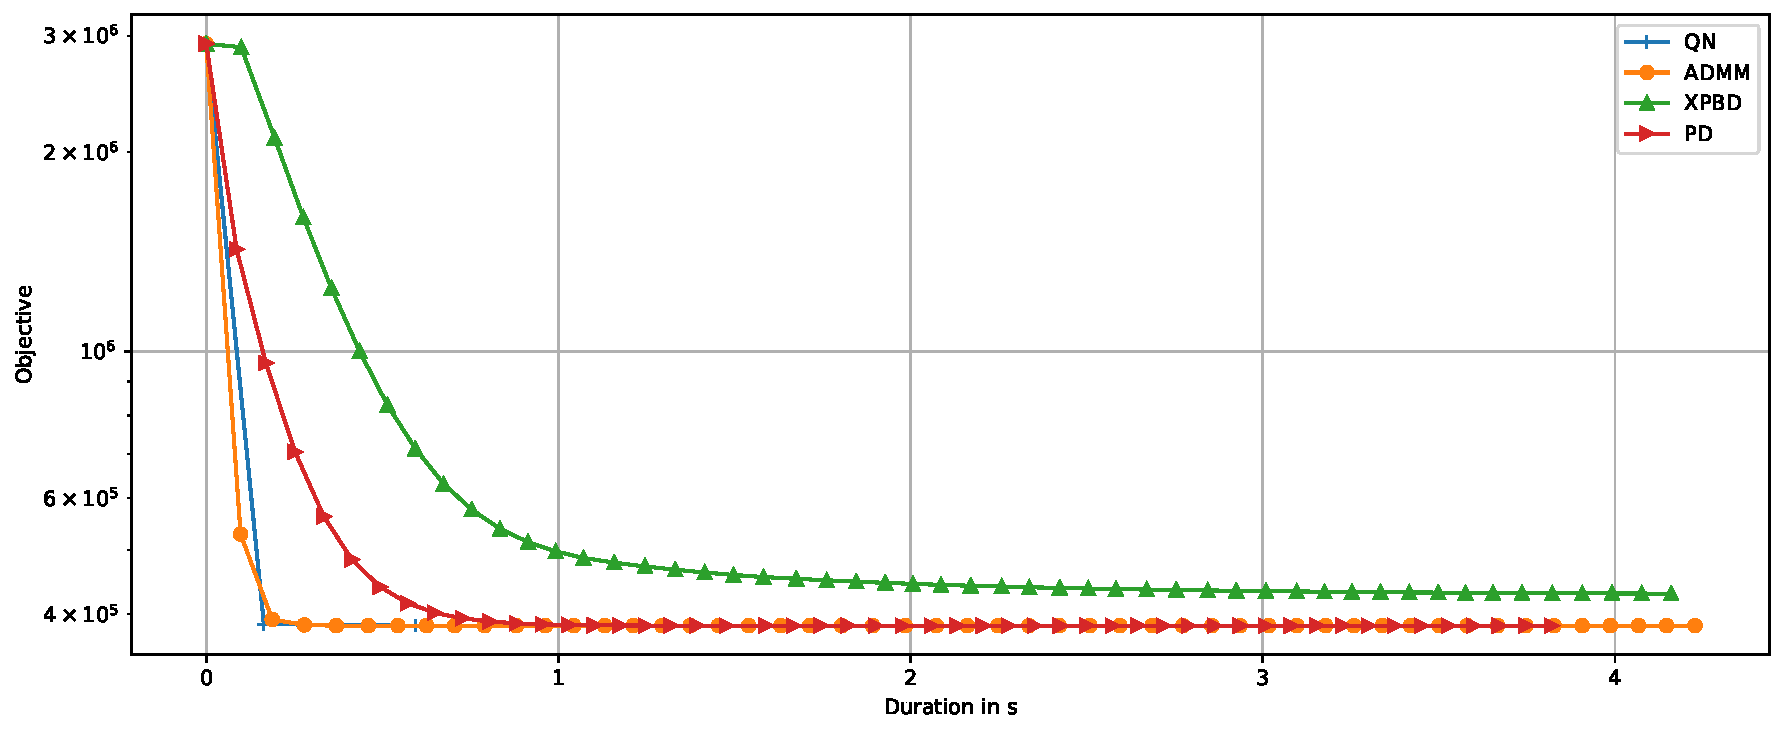
\includegraphics[width=\textwidth]{figures/strain_beam_untwist_objectives_time.pdf}
    \caption{Values of the objective function of the variational form of implicit Euler integration (\cref{eq:variational-implicit}) over the iterations of a single solve (time step 
        \SI{1e-2}{\second}) for an untwisting beam with strain constraints.}
    \label{fig:strain-beam-untwist-objectives-time}
\end{figure}

% TODO:
% - Exchange plots and descriptions in text, use 1000 iterations and log scale.
% - Issues with global angular and linear momentum 
% - Fixed beam scenario and XPBD's lack of punishment for moving away from inertial positions
% - ADMM weights for neohookean model
% - XPBD formulations for neohookean model (incompressibility, stability)
% - Iteration times XPBD solvers
